\documentclass[twoside]{book}

% Packages required by doxygen
\usepackage{fixltx2e}
\usepackage{calc}
\usepackage{doxygen}
\usepackage[export]{adjustbox} % also loads graphicx
\usepackage{graphicx}
\usepackage[utf8]{inputenc}
\usepackage{makeidx}
\usepackage{multicol}
\usepackage{multirow}
\PassOptionsToPackage{warn}{textcomp}
\usepackage{textcomp}
\usepackage[nointegrals]{wasysym}
\usepackage[table]{xcolor}

% Font selection
\usepackage[T1]{fontenc}
\usepackage[scaled=.90]{helvet}
\usepackage{courier}
\usepackage{amssymb}
\usepackage{sectsty}
\renewcommand{\familydefault}{\sfdefault}
\allsectionsfont{%
  \fontseries{bc}\selectfont%
  \color{darkgray}%
}
\renewcommand{\DoxyLabelFont}{%
  \fontseries{bc}\selectfont%
  \color{darkgray}%
}
\newcommand{\+}{\discretionary{\mbox{\scriptsize$\hookleftarrow$}}{}{}}

% Page & text layout
\usepackage{geometry}
\geometry{%
  a4paper,%
  top=2.5cm,%
  bottom=2.5cm,%
  left=2.5cm,%
  right=2.5cm%
}
\tolerance=750
\hfuzz=15pt
\hbadness=750
\setlength{\emergencystretch}{15pt}
\setlength{\parindent}{0cm}
\setlength{\parskip}{3ex plus 2ex minus 2ex}
\makeatletter
\renewcommand{\paragraph}{%
  \@startsection{paragraph}{4}{0ex}{-1.0ex}{1.0ex}{%
    \normalfont\normalsize\bfseries\SS@parafont%
  }%
}
\renewcommand{\subparagraph}{%
  \@startsection{subparagraph}{5}{0ex}{-1.0ex}{1.0ex}{%
    \normalfont\normalsize\bfseries\SS@subparafont%
  }%
}
\makeatother

% Headers & footers
\usepackage{fancyhdr}
\pagestyle{fancyplain}
\fancyhead[LE]{\fancyplain{}{\bfseries\thepage}}
\fancyhead[CE]{\fancyplain{}{}}
\fancyhead[RE]{\fancyplain{}{\bfseries\leftmark}}
\fancyhead[LO]{\fancyplain{}{\bfseries\rightmark}}
\fancyhead[CO]{\fancyplain{}{}}
\fancyhead[RO]{\fancyplain{}{\bfseries\thepage}}
\fancyfoot[LE]{\fancyplain{}{}}
\fancyfoot[CE]{\fancyplain{}{}}
\fancyfoot[RE]{\fancyplain{}{\bfseries\scriptsize Generated by Doxygen }}
\fancyfoot[LO]{\fancyplain{}{\bfseries\scriptsize Generated by Doxygen }}
\fancyfoot[CO]{\fancyplain{}{}}
\fancyfoot[RO]{\fancyplain{}{}}
\renewcommand{\footrulewidth}{0.4pt}
\renewcommand{\chaptermark}[1]{%
  \markboth{#1}{}%
}
\renewcommand{\sectionmark}[1]{%
  \markright{\thesection\ #1}%
}

% Indices & bibliography
\usepackage{natbib}
\usepackage[titles]{tocloft}
\setcounter{tocdepth}{3}
\setcounter{secnumdepth}{5}
\makeindex

% Hyperlinks (required, but should be loaded last)
\usepackage{ifpdf}
\ifpdf
  \usepackage[pdftex,pagebackref=true]{hyperref}
\else
  \usepackage[ps2pdf,pagebackref=true]{hyperref}
\fi
\hypersetup{%
  colorlinks=true,%
  linkcolor=blue,%
  citecolor=blue,%
  unicode%
}

% Custom commands
\newcommand{\clearemptydoublepage}{%
  \newpage{\pagestyle{empty}\cleardoublepage}%
}

\usepackage{caption}
\captionsetup{labelsep=space,justification=centering,font={bf},singlelinecheck=off,skip=4pt,position=top}

%===== C O N T E N T S =====

\begin{document}

% Titlepage & ToC
\hypersetup{pageanchor=false,
             bookmarksnumbered=true,
             pdfencoding=unicode
            }
\pagenumbering{alph}
\begin{titlepage}
\vspace*{7cm}
\begin{center}%
{\Large Existenzia }\\
\vspace*{1cm}
{\large Generated by Doxygen 1.8.14}\\
\end{center}
\end{titlepage}
\clearemptydoublepage
\pagenumbering{roman}
\tableofcontents
\clearemptydoublepage
\pagenumbering{arabic}
\hypersetup{pageanchor=true}

%--- Begin generated contents ---
\chapter{Hierarchical Index}
\section{Class Hierarchy}
This inheritance list is sorted roughly, but not completely, alphabetically\+:\begin{DoxyCompactList}
\item \contentsline{section}{A\+Core}{\pageref{structACore}}{}
\item \contentsline{section}{A\+H\+T\+T\+P\+Module}{\pageref{classAHTTPModule}}{}
\item \contentsline{section}{A\+Loader}{\pageref{classALoader}}{}
\item \contentsline{section}{A\+Module}{\pageref{classAModule}}{}
\item \contentsline{section}{xzia\+:\+:A\+Module}{\pageref{classxzia_1_1AModule}}{}
\begin{DoxyCompactList}
\item \contentsline{section}{xzia\+:\+:A\+H\+T\+T\+P\+Module}{\pageref{classxzia_1_1AHTTPModule}}{}
\item \contentsline{section}{xzia\+:\+:A\+Shared\+Module}{\pageref{classxzia_1_1ASharedModule}}{}
\begin{DoxyCompactList}
\item \contentsline{section}{xzia\+:\+:A\+Protected\+Module}{\pageref{classxzia_1_1AProtectedModule}}{}
\end{DoxyCompactList}
\end{DoxyCompactList}
\item \contentsline{section}{A\+Module\+Manager}{\pageref{classAModuleManager}}{}
\item \contentsline{section}{A\+Protected\+Module}{\pageref{classAProtectedModule}}{}
\item \contentsline{section}{A\+Shared\+Module}{\pageref{classASharedModule}}{}
\item \contentsline{section}{A\+Task}{\pageref{classATask}}{}
\item \contentsline{section}{A\+Task\+Factory}{\pageref{classATaskFactory}}{}
\item \contentsline{section}{A\+Thread\+Pool}{\pageref{classAThreadPool}}{}
\item \contentsline{section}{Client}{\pageref{structClient}}{}
\item \contentsline{section}{Data\+Store}{\pageref{classDataStore}}{}
\item \contentsline{section}{xzia\+:\+:Data\+Store}{\pageref{classxzia_1_1DataStore}}{}
\item \contentsline{section}{xzia\+:\+:I\+Config\+Loader}{\pageref{classxzia_1_1IConfigLoader}}{}
\item \contentsline{section}{I\+Config\+Loader}{\pageref{classIConfigLoader}}{}
\item \contentsline{section}{xzia\+:\+:I\+Core}{\pageref{classxzia_1_1ICore}}{}
\begin{DoxyCompactList}
\item \contentsline{section}{xzia\+:\+:A\+Core}{\pageref{classxzia_1_1ACore}}{}
\end{DoxyCompactList}
\item \contentsline{section}{I\+Core}{\pageref{classICore}}{}
\item \contentsline{section}{xzia\+:\+:I\+Loader}{\pageref{classxzia_1_1ILoader}}{}
\begin{DoxyCompactList}
\item \contentsline{section}{xzia\+:\+:A\+Loader}{\pageref{classxzia_1_1ALoader}}{}
\end{DoxyCompactList}
\item \contentsline{section}{I\+Loader}{\pageref{classILoader}}{}
\item \contentsline{section}{I\+Module\+Manager}{\pageref{classIModuleManager}}{}
\item \contentsline{section}{xzia\+:\+:I\+Module\+Manager}{\pageref{classxzia_1_1IModuleManager}}{}
\begin{DoxyCompactList}
\item \contentsline{section}{xzia\+:\+:A\+Module\+Manager}{\pageref{classxzia_1_1AModuleManager}}{}
\end{DoxyCompactList}
\item \contentsline{section}{xzia\+:\+:I\+Network}{\pageref{classxzia_1_1INetwork}}{}
\item \contentsline{section}{I\+Network}{\pageref{classINetwork}}{}
\item \contentsline{section}{I\+Task}{\pageref{classITask}}{}
\item \contentsline{section}{xzia\+:\+:I\+Task}{\pageref{classxzia_1_1ITask}}{}
\begin{DoxyCompactList}
\item \contentsline{section}{xzia\+:\+:A\+Task}{\pageref{classxzia_1_1ATask}}{}
\end{DoxyCompactList}
\item \contentsline{section}{I\+Task\+Factory}{\pageref{classITaskFactory}}{}
\item \contentsline{section}{xzia\+:\+:I\+Task\+Factory}{\pageref{classxzia_1_1ITaskFactory}}{}
\begin{DoxyCompactList}
\item \contentsline{section}{xzia\+:\+:A\+Task\+Factory}{\pageref{classxzia_1_1ATaskFactory}}{}
\end{DoxyCompactList}
\item \contentsline{section}{I\+Thread\+Pool}{\pageref{classIThreadPool}}{}
\item \contentsline{section}{xzia\+:\+:I\+Thread\+Pool}{\pageref{classxzia_1_1IThreadPool}}{}
\begin{DoxyCompactList}
\item \contentsline{section}{xzia\+:\+:A\+Thread\+Pool}{\pageref{classxzia_1_1AThreadPool}}{}
\end{DoxyCompactList}
\item \contentsline{section}{Message}{\pageref{structMessage}}{}
\item \contentsline{section}{xzia\+:\+:Message}{\pageref{structxzia_1_1Message}}{}
\begin{DoxyCompactList}
\item \contentsline{section}{xzia\+:\+:Request}{\pageref{structxzia_1_1Request}}{}
\item \contentsline{section}{xzia\+:\+:Response}{\pageref{structxzia_1_1Response}}{}
\end{DoxyCompactList}
\item \contentsline{section}{Request}{\pageref{structRequest}}{}
\item \contentsline{section}{Response}{\pageref{structResponse}}{}
\end{DoxyCompactList}

\chapter{Class Index}
\section{Class List}
Here are the classes, structs, unions and interfaces with brief descriptions\+:\begin{DoxyCompactList}
\item\contentsline{section}{\mbox{\hyperlink{classxzia_1_1ACore}{xzia\+::\+A\+Core}} }{\pageref{classxzia_1_1ACore}}{}
\item\contentsline{section}{\mbox{\hyperlink{structACore}{A\+Core}} }{\pageref{structACore}}{}
\item\contentsline{section}{\mbox{\hyperlink{classADataStore}{A\+Data\+Store}} }{\pageref{classADataStore}}{}
\item\contentsline{section}{\mbox{\hyperlink{classxzia_1_1AHTTPModule}{xzia\+::\+A\+H\+T\+T\+P\+Module}} }{\pageref{classxzia_1_1AHTTPModule}}{}
\item\contentsline{section}{\mbox{\hyperlink{classAHTTPModule}{A\+H\+T\+T\+P\+Module}} }{\pageref{classAHTTPModule}}{}
\item\contentsline{section}{\mbox{\hyperlink{classxzia_1_1ALoader}{xzia\+::\+A\+Loader}} }{\pageref{classxzia_1_1ALoader}}{}
\item\contentsline{section}{\mbox{\hyperlink{classALoader}{A\+Loader}} }{\pageref{classALoader}}{}
\item\contentsline{section}{\mbox{\hyperlink{classAModule}{A\+Module}} }{\pageref{classAModule}}{}
\item\contentsline{section}{\mbox{\hyperlink{classxzia_1_1AModule}{xzia\+::\+A\+Module}} }{\pageref{classxzia_1_1AModule}}{}
\item\contentsline{section}{\mbox{\hyperlink{classAModuleManager}{A\+Module\+Manager}} }{\pageref{classAModuleManager}}{}
\item\contentsline{section}{\mbox{\hyperlink{classxzia_1_1AModuleManager}{xzia\+::\+A\+Module\+Manager}} }{\pageref{classxzia_1_1AModuleManager}}{}
\item\contentsline{section}{\mbox{\hyperlink{classAProtectedModule}{A\+Protected\+Module}} }{\pageref{classAProtectedModule}}{}
\item\contentsline{section}{\mbox{\hyperlink{classxzia_1_1AProtectedModule}{xzia\+::\+A\+Protected\+Module}} }{\pageref{classxzia_1_1AProtectedModule}}{}
\item\contentsline{section}{\mbox{\hyperlink{classASharedModule}{A\+Shared\+Module}} }{\pageref{classASharedModule}}{}
\item\contentsline{section}{\mbox{\hyperlink{classxzia_1_1ASharedModule}{xzia\+::\+A\+Shared\+Module}} }{\pageref{classxzia_1_1ASharedModule}}{}
\item\contentsline{section}{\mbox{\hyperlink{classxzia_1_1ATask}{xzia\+::\+A\+Task}} }{\pageref{classxzia_1_1ATask}}{}
\item\contentsline{section}{\mbox{\hyperlink{classATask}{A\+Task}} }{\pageref{classATask}}{}
\item\contentsline{section}{\mbox{\hyperlink{classxzia_1_1ATaskFactory}{xzia\+::\+A\+Task\+Factory}} }{\pageref{classxzia_1_1ATaskFactory}}{}
\item\contentsline{section}{\mbox{\hyperlink{classxzia_1_1AThreadPool}{xzia\+::\+A\+Thread\+Pool}} }{\pageref{classxzia_1_1AThreadPool}}{}
\item\contentsline{section}{\mbox{\hyperlink{classAThreadPool}{A\+Thread\+Pool}} }{\pageref{classAThreadPool}}{}
\item\contentsline{section}{\mbox{\hyperlink{structClient}{Client}} }{\pageref{structClient}}{}
\item\contentsline{section}{\mbox{\hyperlink{classxzia_1_1DataStore}{xzia\+::\+Data\+Store}} }{\pageref{classxzia_1_1DataStore}}{}
\item\contentsline{section}{\mbox{\hyperlink{classxzia_1_1IConfigLoader}{xzia\+::\+I\+Config\+Loader}} }{\pageref{classxzia_1_1IConfigLoader}}{}
\item\contentsline{section}{\mbox{\hyperlink{classIConfigLoader}{I\+Config\+Loader}} }{\pageref{classIConfigLoader}}{}
\item\contentsline{section}{\mbox{\hyperlink{classxzia_1_1ICore}{xzia\+::\+I\+Core}} }{\pageref{classxzia_1_1ICore}}{}
\item\contentsline{section}{\mbox{\hyperlink{classICore}{I\+Core}} }{\pageref{classICore}}{}
\item\contentsline{section}{\mbox{\hyperlink{classILoader}{I\+Loader}} }{\pageref{classILoader}}{}
\item\contentsline{section}{\mbox{\hyperlink{classxzia_1_1ILoader}{xzia\+::\+I\+Loader}} }{\pageref{classxzia_1_1ILoader}}{}
\item\contentsline{section}{\mbox{\hyperlink{classIModuleManager}{I\+Module\+Manager}} }{\pageref{classIModuleManager}}{}
\item\contentsline{section}{\mbox{\hyperlink{classxzia_1_1IModuleManager}{xzia\+::\+I\+Module\+Manager}} }{\pageref{classxzia_1_1IModuleManager}}{}
\item\contentsline{section}{\mbox{\hyperlink{classxzia_1_1INetwork}{xzia\+::\+I\+Network}} }{\pageref{classxzia_1_1INetwork}}{}
\item\contentsline{section}{\mbox{\hyperlink{classINetwork}{I\+Network}} }{\pageref{classINetwork}}{}
\item\contentsline{section}{\mbox{\hyperlink{classITask}{I\+Task}} }{\pageref{classITask}}{}
\item\contentsline{section}{\mbox{\hyperlink{classxzia_1_1ITask}{xzia\+::\+I\+Task}} }{\pageref{classxzia_1_1ITask}}{}
\item\contentsline{section}{\mbox{\hyperlink{classxzia_1_1ITaskFactory}{xzia\+::\+I\+Task\+Factory}} }{\pageref{classxzia_1_1ITaskFactory}}{}
\item\contentsline{section}{\mbox{\hyperlink{classIThreadPool}{I\+Thread\+Pool}} }{\pageref{classIThreadPool}}{}
\item\contentsline{section}{\mbox{\hyperlink{classxzia_1_1IThreadPool}{xzia\+::\+I\+Thread\+Pool}} }{\pageref{classxzia_1_1IThreadPool}}{}
\item\contentsline{section}{\mbox{\hyperlink{structxzia_1_1Message}{xzia\+::\+Message}} }{\pageref{structxzia_1_1Message}}{}
\item\contentsline{section}{\mbox{\hyperlink{structMessage}{Message}} }{\pageref{structMessage}}{}
\item\contentsline{section}{\mbox{\hyperlink{structxzia_1_1Request}{xzia\+::\+Request}} }{\pageref{structxzia_1_1Request}}{}
\item\contentsline{section}{\mbox{\hyperlink{structRequest}{Request}} }{\pageref{structRequest}}{}
\item\contentsline{section}{\mbox{\hyperlink{structxzia_1_1Response}{xzia\+::\+Response}} }{\pageref{structxzia_1_1Response}}{}
\item\contentsline{section}{\mbox{\hyperlink{structResponse}{Response}} }{\pageref{structResponse}}{}
\end{DoxyCompactList}

\chapter{File Index}
\section{File List}
Here is a list of all documented files with brief descriptions\+:\begin{DoxyCompactList}
\item\contentsline{section}{/home/edouard/\+Documents/2017/\+Z\+I\+A/\+Existen\+Z\+I\+A/\+A\+P\+I/include/client/\mbox{\hyperlink{Client_8hpp}{Client.\+hpp}} \\*Typedef the socket \mbox{\hyperlink{structClient}{Client}} as an int }{\pageref{Client_8hpp}}{}
\item\contentsline{section}{/home/edouard/\+Documents/2017/\+Z\+I\+A/\+Existen\+Z\+I\+A/\+A\+P\+I/include/core/\mbox{\hyperlink{ACore_8hpp}{A\+Core.\+hpp}} \\*Kernel of the A\+PI, \mbox{\hyperlink{structACore}{A\+Core}} is the class linked to all other classes }{\pageref{ACore_8hpp}}{}
\item\contentsline{section}{/home/edouard/\+Documents/2017/\+Z\+I\+A/\+Existen\+Z\+I\+A/\+A\+P\+I/include/core/\mbox{\hyperlink{ICore_8hpp}{I\+Core.\+hpp}} \\*Interface of the main class of the A\+PI }{\pageref{ICore_8hpp}}{}
\item\contentsline{section}{/home/edouard/\+Documents/2017/\+Z\+I\+A/\+Existen\+Z\+I\+A/\+A\+P\+I/include/http/\mbox{\hyperlink{Message_8hpp}{Message.\+hpp}} \\*\mbox{\hyperlink{structMessage}{Message}} is a structure which contain all the information about the request. It can be either a request to ask information or a response for the return of a request }{\pageref{Message_8hpp}}{}
\item\contentsline{section}{/home/edouard/\+Documents/2017/\+Z\+I\+A/\+Existen\+Z\+I\+A/\+A\+P\+I/include/http/\mbox{\hyperlink{Request_8hpp}{Request.\+hpp}} \\*\mbox{\hyperlink{structRequest}{Request}} is a specific message which goal is to ask something and wait for a response }{\pageref{Request_8hpp}}{}
\item\contentsline{section}{/home/edouard/\+Documents/2017/\+Z\+I\+A/\+Existen\+Z\+I\+A/\+A\+P\+I/include/http/\mbox{\hyperlink{Response_8hpp}{Response.\+hpp}} \\*\mbox{\hyperlink{structResponse}{Response}} is a specific message which goal is to return a message containing the result code of the task asked }{\pageref{Response_8hpp}}{}
\item\contentsline{section}{/home/edouard/\+Documents/2017/\+Z\+I\+A/\+Existen\+Z\+I\+A/\+A\+P\+I/include/loader/\mbox{\hyperlink{ALoader_8hpp}{A\+Loader.\+hpp}} \\*\mbox{\hyperlink{classALoader}{A\+Loader}} manages the dynamic loading of the modules and the configuration of those according to the configuration loader }{\pageref{ALoader_8hpp}}{}
\item\contentsline{section}{/home/edouard/\+Documents/2017/\+Z\+I\+A/\+Existen\+Z\+I\+A/\+A\+P\+I/include/loader/\mbox{\hyperlink{IConfigLoader_8hpp}{I\+Config\+Loader.\+hpp}} }{\pageref{IConfigLoader_8hpp}}{}
\item\contentsline{section}{/home/edouard/\+Documents/2017/\+Z\+I\+A/\+Existen\+Z\+I\+A/\+A\+P\+I/include/loader/\mbox{\hyperlink{ILoader_8hpp}{I\+Loader.\+hpp}} }{\pageref{ILoader_8hpp}}{}
\item\contentsline{section}{/home/edouard/\+Documents/2017/\+Z\+I\+A/\+Existen\+Z\+I\+A/\+A\+P\+I/include/modules/\mbox{\hyperlink{AHTTPModule_8hpp}{A\+H\+T\+T\+P\+Module.\+hpp}} \\*Standard module that is used in the task execution list }{\pageref{AHTTPModule_8hpp}}{}
\item\contentsline{section}{/home/edouard/\+Documents/2017/\+Z\+I\+A/\+Existen\+Z\+I\+A/\+A\+P\+I/include/modules/\mbox{\hyperlink{AModule_8hpp}{A\+Module.\+hpp}} \\*This is the most basic module, you should {\itshape never} directly inherit from this class, use the other module Abstract Classes \+: \mbox{\hyperlink{classAHTTPModule}{A\+H\+T\+T\+P\+Module}}, \mbox{\hyperlink{classASharedModule}{A\+Shared\+Module}} and \mbox{\hyperlink{classAProtectedModule}{A\+Protected\+Module}} }{\pageref{AModule_8hpp}}{}
\item\contentsline{section}{/home/edouard/\+Documents/2017/\+Z\+I\+A/\+Existen\+Z\+I\+A/\+A\+P\+I/include/modules/\mbox{\hyperlink{AModuleManager_8hpp}{A\+Module\+Manager.\+hpp}} \\*The module manager has ownership of all modules and is responsible for reloading them. It creates copies of basic modules and pass references to shared ones }{\pageref{AModuleManager_8hpp}}{}
\item\contentsline{section}{/home/edouard/\+Documents/2017/\+Z\+I\+A/\+Existen\+Z\+I\+A/\+A\+P\+I/include/modules/\mbox{\hyperlink{AProtectedModule_8hpp}{A\+Protected\+Module.\+hpp}} }{\pageref{AProtectedModule_8hpp}}{}
\item\contentsline{section}{/home/edouard/\+Documents/2017/\+Z\+I\+A/\+Existen\+Z\+I\+A/\+A\+P\+I/include/modules/\mbox{\hyperlink{ASharedModule_8hpp}{A\+Shared\+Module.\+hpp}} \\*This module is protected by a mutex and can be accessed through threads. The inheriting class must implement its logic in the safe\+Process method instead of the process method }{\pageref{ASharedModule_8hpp}}{}
\item\contentsline{section}{/home/edouard/\+Documents/2017/\+Z\+I\+A/\+Existen\+Z\+I\+A/\+A\+P\+I/include/modules/{\bfseries Data\+Store.\+hpp} }{\pageref{DataStore_8hpp}}{}
\item\contentsline{section}{/home/edouard/\+Documents/2017/\+Z\+I\+A/\+Existen\+Z\+I\+A/\+A\+P\+I/include/modules/\mbox{\hyperlink{IModuleManager_8hpp}{I\+Module\+Manager.\+hpp}} \\*Interface of the module manager }{\pageref{IModuleManager_8hpp}}{}
\item\contentsline{section}{/home/edouard/\+Documents/2017/\+Z\+I\+A/\+Existen\+Z\+I\+A/\+A\+P\+I/include/modules/\mbox{\hyperlink{Step_8hpp}{Step.\+hpp}} }{\pageref{Step_8hpp}}{}
\item\contentsline{section}{/home/edouard/\+Documents/2017/\+Z\+I\+A/\+Existen\+Z\+I\+A/\+A\+P\+I/include/network/\mbox{\hyperlink{INetwork_8hpp}{I\+Network.\+hpp}} \\*Network is the class which link Core (Arrival of a message, and send the message response) to the client }{\pageref{INetwork_8hpp}}{}
\item\contentsline{section}{/home/edouard/\+Documents/2017/\+Z\+I\+A/\+Existen\+Z\+I\+A/\+A\+P\+I/include/task/\mbox{\hyperlink{ATask_8hpp}{A\+Task.\+hpp}} \\*\mbox{\hyperlink{classATask}{A\+Task}} represent the module list defined by the \mbox{\hyperlink{structRequest}{Request}} passed in the Constructor }{\pageref{ATask_8hpp}}{}
\item\contentsline{section}{/home/edouard/\+Documents/2017/\+Z\+I\+A/\+Existen\+Z\+I\+A/\+A\+P\+I/include/task/{\bfseries A\+Task\+Factory.\+hpp} }{\pageref{ATaskFactory_8hpp}}{}
\item\contentsline{section}{/home/edouard/\+Documents/2017/\+Z\+I\+A/\+Existen\+Z\+I\+A/\+A\+P\+I/include/task/\mbox{\hyperlink{ITask_8hpp}{I\+Task.\+hpp}} \\*The \mbox{\hyperlink{classITask}{I\+Task}} Interface manage the communication between request and client. It also links all the different module specific to the request }{\pageref{ITask_8hpp}}{}
\item\contentsline{section}{/home/edouard/\+Documents/2017/\+Z\+I\+A/\+Existen\+Z\+I\+A/\+A\+P\+I/include/task/{\bfseries I\+Task\+Factory.\+hpp} }{\pageref{ITaskFactory_8hpp}}{}
\item\contentsline{section}{/home/edouard/\+Documents/2017/\+Z\+I\+A/\+Existen\+Z\+I\+A/\+A\+P\+I/include/thread/\mbox{\hyperlink{AThreadPool_8hpp}{A\+Thread\+Pool.\+hpp}} \\*\mbox{\hyperlink{classAThreadPool}{A\+Thread\+Pool}} is our manager of all the thread we are going to use during the process of a task }{\pageref{AThreadPool_8hpp}}{}
\item\contentsline{section}{/home/edouard/\+Documents/2017/\+Z\+I\+A/\+Existen\+Z\+I\+A/\+A\+P\+I/include/thread/\mbox{\hyperlink{IThreadPool_8hpp}{I\+Thread\+Pool.\+hpp}} \\*Interface of our manager of threads }{\pageref{IThreadPool_8hpp}}{}
\item\contentsline{section}{/home/edouard/\+Documents/2017/\+Z\+I\+A/\+Existen\+Z\+I\+A/\+A\+P\+I/include/thread/\mbox{\hyperlink{ThreadState_8hpp}{Thread\+State.\+hpp}} \\*Enum class representing the thread\textquotesingle{}s work\+State }{\pageref{ThreadState_8hpp}}{}
\end{DoxyCompactList}

\chapter{Class Documentation}
\hypertarget{classxzia_1_1ACore}{}\section{xzia\+:\+:A\+Core Class Reference}
\label{classxzia_1_1ACore}\index{xzia\+::\+A\+Core@{xzia\+::\+A\+Core}}
Inheritance diagram for xzia\+:\+:A\+Core\+:\begin{figure}[H]
\begin{center}
\leavevmode
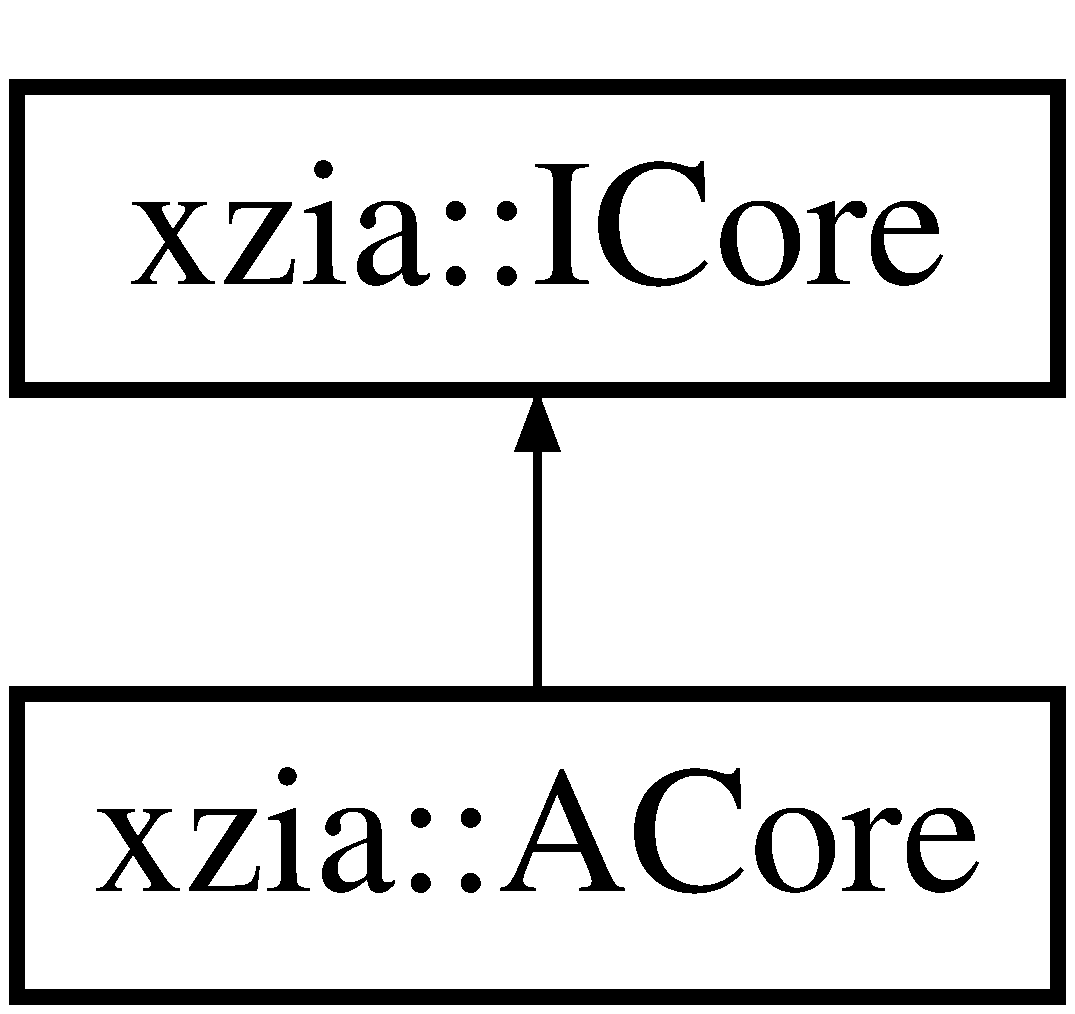
\includegraphics[height=2.000000cm]{classxzia_1_1ACore}
\end{center}
\end{figure}
\subsection*{Public Member Functions}
\begin{DoxyCompactItemize}
\item 
\mbox{\hyperlink{classxzia_1_1ACore_a615436a95f788dd92d545e10a1d4b2c3}{A\+Core}} (std\+::string const \&config)
\begin{DoxyCompactList}\small\item\em Constructor of the class \mbox{\hyperlink{classxzia_1_1ACore}{A\+Core}}. We set a configuration representing by a string. \end{DoxyCompactList}\end{DoxyCompactItemize}
\subsection*{Protected Attributes}
\begin{DoxyCompactItemize}
\item 
\mbox{\Hypertarget{classxzia_1_1ACore_ae22e66acfe4f3257eb10019fa21a56f2}\label{classxzia_1_1ACore_ae22e66acfe4f3257eb10019fa21a56f2}} 
std\+::unique\+\_\+ptr$<$ \mbox{\hyperlink{classxzia_1_1ILoader}{I\+Loader}} $>$ {\bfseries loader}
\item 
\mbox{\Hypertarget{classxzia_1_1ACore_a1168c0799674e15ef09c100d0aaaa0bb}\label{classxzia_1_1ACore_a1168c0799674e15ef09c100d0aaaa0bb}} 
std\+::unique\+\_\+ptr$<$ \mbox{\hyperlink{classxzia_1_1AModuleManager}{A\+Module\+Manager}} $>$ {\bfseries module\+Manager}
\item 
\mbox{\Hypertarget{classxzia_1_1ACore_aa1388a6e0bf6f19a6d59d63145b9fc36}\label{classxzia_1_1ACore_aa1388a6e0bf6f19a6d59d63145b9fc36}} 
std\+::unique\+\_\+ptr$<$ \mbox{\hyperlink{classxzia_1_1AThreadPool}{A\+Thread\+Pool}} $>$ {\bfseries thread\+Pool}
\item 
\mbox{\Hypertarget{classxzia_1_1ACore_a096cbf3ea8cc7a9eb2856f14ad3d9c87}\label{classxzia_1_1ACore_a096cbf3ea8cc7a9eb2856f14ad3d9c87}} 
std\+::unique\+\_\+ptr$<$ \mbox{\hyperlink{classxzia_1_1INetwork}{I\+Network}} $>$ {\bfseries network}
\item 
\mbox{\Hypertarget{classxzia_1_1ACore_a2d03c49c10d23d220c60bf8d098d30ac}\label{classxzia_1_1ACore_a2d03c49c10d23d220c60bf8d098d30ac}} 
std\+::unique\+\_\+ptr$<$ \mbox{\hyperlink{classxzia_1_1ATaskFactory}{A\+Task\+Factory}} $>$ {\bfseries task\+Factory}
\item 
\mbox{\Hypertarget{classxzia_1_1ACore_a079015b2ad82d2f5eb918589421c26c8}\label{classxzia_1_1ACore_a079015b2ad82d2f5eb918589421c26c8}} 
std\+::string {\bfseries config\+File}
\end{DoxyCompactItemize}


\subsection{Constructor \& Destructor Documentation}
\mbox{\Hypertarget{classxzia_1_1ACore_a615436a95f788dd92d545e10a1d4b2c3}\label{classxzia_1_1ACore_a615436a95f788dd92d545e10a1d4b2c3}} 
\index{xzia\+::\+A\+Core@{xzia\+::\+A\+Core}!A\+Core@{A\+Core}}
\index{A\+Core@{A\+Core}!xzia\+::\+A\+Core@{xzia\+::\+A\+Core}}
\subsubsection{\texorpdfstring{A\+Core()}{ACore()}}
{\footnotesize\ttfamily A\+Core\+::\+A\+Core (\begin{DoxyParamCaption}\item[{std\+::string const \&}]{config }\end{DoxyParamCaption})\hspace{0.3cm}{\ttfamily [explicit]}}



Constructor of the class \mbox{\hyperlink{classxzia_1_1ACore}{A\+Core}}. We set a configuration representing by a string. 


\begin{DoxyParams}{Parameters}
{\em config} & Configuration of the core \\
\hline
\end{DoxyParams}


The documentation for this class was generated from the following files\+:\begin{DoxyCompactItemize}
\item 
/home/edouard/\+Documents/2017/\+Z\+I\+A/\+Existen\+Z\+I\+A/\+A\+P\+I/include/core/\mbox{\hyperlink{ACore_8hpp}{A\+Core.\+hpp}}\item 
/home/edouard/\+Documents/2017/\+Z\+I\+A/\+Existen\+Z\+I\+A/\+A\+P\+I/src/core/A\+Core.\+cpp\end{DoxyCompactItemize}

\hypertarget{structACore}{}\section{A\+Core Struct Reference}
\label{structACore}\index{A\+Core@{A\+Core}}


The documentation for this struct was generated from the following file\+:\begin{DoxyCompactItemize}
\item 
/home/edouard/\+Documents/2017/\+Z\+I\+A/\+Existen\+Z\+I\+A/\+A\+P\+I/include/core/\mbox{\hyperlink{ACore_8hpp}{A\+Core.\+hpp}}\end{DoxyCompactItemize}

\hypertarget{classxzia_1_1AHTTPModule}{}\section{xzia\+:\+:A\+H\+T\+T\+P\+Module Class Reference}
\label{classxzia_1_1AHTTPModule}\index{xzia\+::\+A\+H\+T\+T\+P\+Module@{xzia\+::\+A\+H\+T\+T\+P\+Module}}
Inheritance diagram for xzia\+:\+:A\+H\+T\+T\+P\+Module\+:\begin{figure}[H]
\begin{center}
\leavevmode
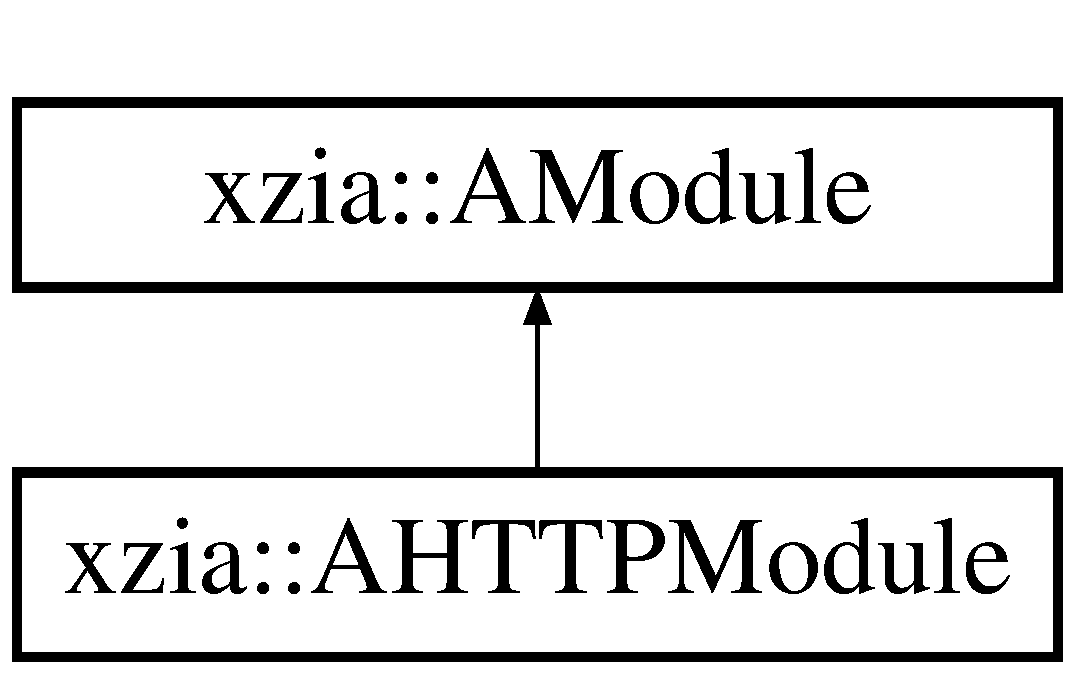
\includegraphics[height=2.000000cm]{classxzia_1_1AHTTPModule}
\end{center}
\end{figure}
\subsection*{Public Member Functions}
\begin{DoxyCompactItemize}
\item 
\mbox{\Hypertarget{classxzia_1_1AHTTPModule_abb342531b0bfb055f8d79c8634622e97}\label{classxzia_1_1AHTTPModule_abb342531b0bfb055f8d79c8634622e97}} 
{\bfseries A\+H\+T\+T\+P\+Module} (std\+::string const \&name, \mbox{\hyperlink{classxzia_1_1AModuleManager}{A\+Module\+Manager}} \&manager)
\item 
\mbox{\Hypertarget{classxzia_1_1AHTTPModule_ad2eec7ec7828720f511d204a15c3dc9d}\label{classxzia_1_1AHTTPModule_ad2eec7ec7828720f511d204a15c3dc9d}} 
{\bfseries A\+H\+T\+T\+P\+Module} (\mbox{\hyperlink{classxzia_1_1AHTTPModule}{A\+H\+T\+T\+P\+Module}} const \&http\+Module)
\item 
virtual \mbox{\hyperlink{Step_8hpp_a58ad1bb906913f90b95697c49f198770}{Step}} \mbox{\hyperlink{classxzia_1_1AHTTPModule_aec792240cda0e3697184e6271fb3a66b}{process}} (\mbox{\hyperlink{classxzia_1_1ATask}{A\+Task}} \&task)=0
\begin{DoxyCompactList}\small\item\em This method is called by the workers in the \mbox{\hyperlink{classxzia_1_1AThreadPool}{A\+Thread\+Pool}}, the logic of the module shall be coded here. \end{DoxyCompactList}\item 
\mbox{\Hypertarget{classxzia_1_1AHTTPModule_ad4a892371fa598dcda37ffd2c086e9ab}\label{classxzia_1_1AHTTPModule_ad4a892371fa598dcda37ffd2c086e9ab}} 
{\footnotesize template$<$typename T $>$ }\\void \mbox{\hyperlink{classxzia_1_1AHTTPModule_ad4a892371fa598dcda37ffd2c086e9ab}{add\+Data}} (std\+::string const \&key, T data)
\begin{DoxyCompactList}\small\item\em Allows to add data to a module for future use in the Task execution list. Store important data in the store of the module. \end{DoxyCompactList}\end{DoxyCompactItemize}
\subsection*{Protected Attributes}
\begin{DoxyCompactItemize}
\item 
\mbox{\Hypertarget{classxzia_1_1AHTTPModule_a39a53de846e4e012adacfebfdaf2c4db}\label{classxzia_1_1AHTTPModule_a39a53de846e4e012adacfebfdaf2c4db}} 
\mbox{\hyperlink{classxzia_1_1DataStore}{Data\+Store}} {\bfseries data\+Store}
\end{DoxyCompactItemize}
\subsection*{Additional Inherited Members}


\subsection{Member Function Documentation}
\mbox{\Hypertarget{classxzia_1_1AHTTPModule_aec792240cda0e3697184e6271fb3a66b}\label{classxzia_1_1AHTTPModule_aec792240cda0e3697184e6271fb3a66b}} 
\index{xzia\+::\+A\+H\+T\+T\+P\+Module@{xzia\+::\+A\+H\+T\+T\+P\+Module}!process@{process}}
\index{process@{process}!xzia\+::\+A\+H\+T\+T\+P\+Module@{xzia\+::\+A\+H\+T\+T\+P\+Module}}
\subsubsection{\texorpdfstring{process()}{process()}}
{\footnotesize\ttfamily A\+H\+T\+T\+P\+Module\+::process (\begin{DoxyParamCaption}\item[{\mbox{\hyperlink{classxzia_1_1ATask}{A\+Task}} \&}]{task }\end{DoxyParamCaption})\hspace{0.3cm}{\ttfamily [pure virtual]}}



This method is called by the workers in the \mbox{\hyperlink{classxzia_1_1AThreadPool}{A\+Thread\+Pool}}, the logic of the module shall be coded here. 


\begin{DoxyParams}{Parameters}
{\em task} & The Task that is passed through all modules \\
\hline
\end{DoxyParams}
\begin{DoxyReturn}{Returns}
a Step that let the Thread\+Pool know if it can continue to the next module or stop and send a response 
\end{DoxyReturn}


The documentation for this class was generated from the following files\+:\begin{DoxyCompactItemize}
\item 
/home/edouard/\+Documents/2017/\+Z\+I\+A/\+Existen\+Z\+I\+A/\+A\+P\+I/include/modules/\mbox{\hyperlink{AHTTPModule_8hpp}{A\+H\+T\+T\+P\+Module.\+hpp}}\item 
/home/edouard/\+Documents/2017/\+Z\+I\+A/\+Existen\+Z\+I\+A/\+A\+P\+I/src/modules/A\+H\+T\+T\+P\+Module.\+cpp\end{DoxyCompactItemize}

\hypertarget{classAHTTPModule}{}\section{A\+H\+T\+T\+P\+Module Class Reference}
\label{classAHTTPModule}\index{A\+H\+T\+T\+P\+Module@{A\+H\+T\+T\+P\+Module}}


The documentation for this class was generated from the following file\+:\begin{DoxyCompactItemize}
\item 
/home/edouard/\+Documents/2017/\+Z\+I\+A/\+Existen\+Z\+I\+A/\+A\+P\+I/include/modules/\mbox{\hyperlink{AHTTPModule_8hpp}{A\+H\+T\+T\+P\+Module.\+hpp}}\end{DoxyCompactItemize}

\hypertarget{classxzia_1_1ALoader}{}\section{xzia\+:\+:A\+Loader Class Reference}
\label{classxzia_1_1ALoader}\index{xzia\+::\+A\+Loader@{xzia\+::\+A\+Loader}}
Inheritance diagram for xzia\+:\+:A\+Loader\+:\begin{figure}[H]
\begin{center}
\leavevmode
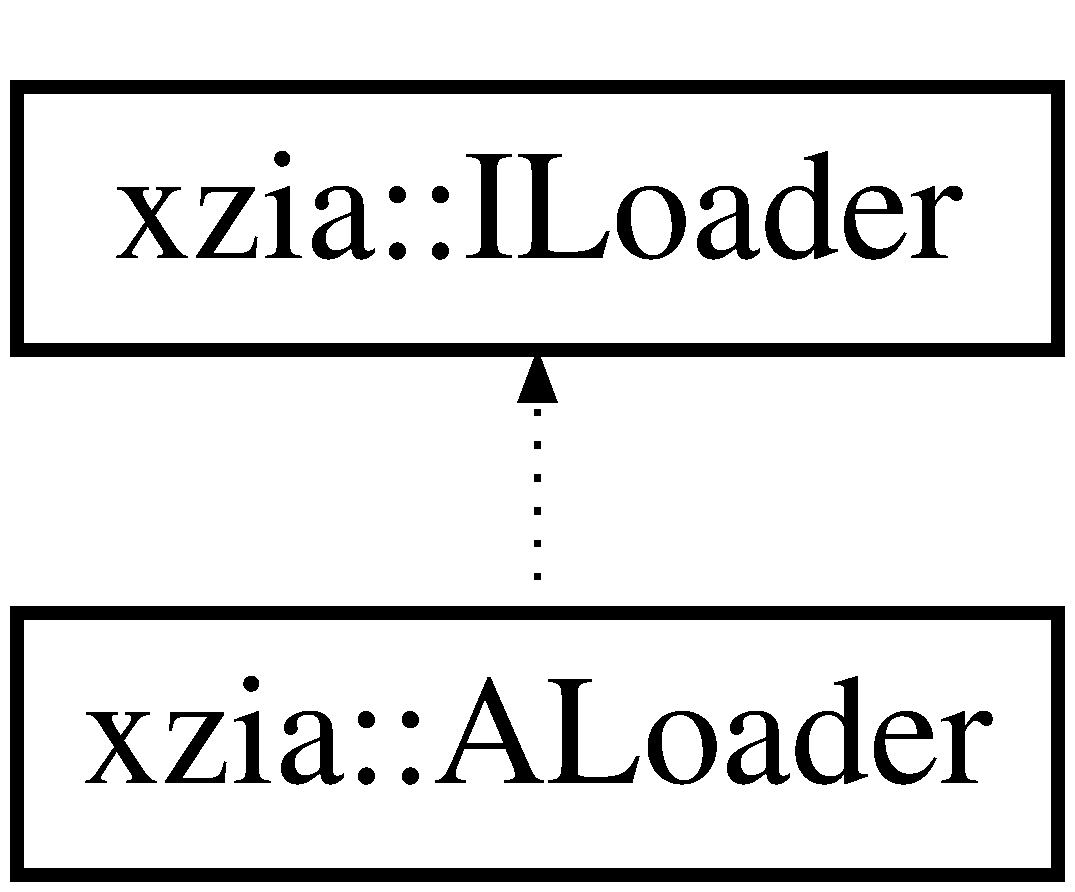
\includegraphics[height=2.000000cm]{classxzia_1_1ALoader}
\end{center}
\end{figure}
\subsection*{Protected Attributes}
\begin{DoxyCompactItemize}
\item 
\mbox{\Hypertarget{classxzia_1_1ALoader_afdc1357bc6a1be8d6f9e5fcb28588fe3}\label{classxzia_1_1ALoader_afdc1357bc6a1be8d6f9e5fcb28588fe3}} 
std\+::unique\+\_\+ptr$<$ \mbox{\hyperlink{classxzia_1_1IConfigLoader}{I\+Config\+Loader}} $>$ {\bfseries config\+Loader}
\end{DoxyCompactItemize}


The documentation for this class was generated from the following file\+:\begin{DoxyCompactItemize}
\item 
/home/edouard/\+Documents/2017/\+Z\+I\+A/\+Existen\+Z\+I\+A/\+A\+P\+I/include/loader/\mbox{\hyperlink{ALoader_8hpp}{A\+Loader.\+hpp}}\end{DoxyCompactItemize}

\hypertarget{classALoader}{}\section{A\+Loader Class Reference}
\label{classALoader}\index{A\+Loader@{A\+Loader}}


The documentation for this class was generated from the following file\+:\begin{DoxyCompactItemize}
\item 
/home/edouard/\+Documents/2017/\+Z\+I\+A/\+Existen\+Z\+I\+A/\+A\+P\+I/include/loader/\mbox{\hyperlink{ALoader_8hpp}{A\+Loader.\+hpp}}\end{DoxyCompactItemize}

\hypertarget{classAModule}{}\section{A\+Module Class Reference}
\label{classAModule}\index{A\+Module@{A\+Module}}


The documentation for this class was generated from the following file\+:\begin{DoxyCompactItemize}
\item 
/home/edouard/\+Documents/2017/\+Z\+I\+A/\+Existen\+Z\+I\+A/\+A\+P\+I/include/modules/\mbox{\hyperlink{AModule_8hpp}{A\+Module.\+hpp}}\end{DoxyCompactItemize}

\hypertarget{classxzia_1_1AModule}{}\section{xzia\+:\+:A\+Module Class Reference}
\label{classxzia_1_1AModule}\index{xzia\+::\+A\+Module@{xzia\+::\+A\+Module}}
Inheritance diagram for xzia\+:\+:A\+Module\+:\begin{figure}[H]
\begin{center}
\leavevmode
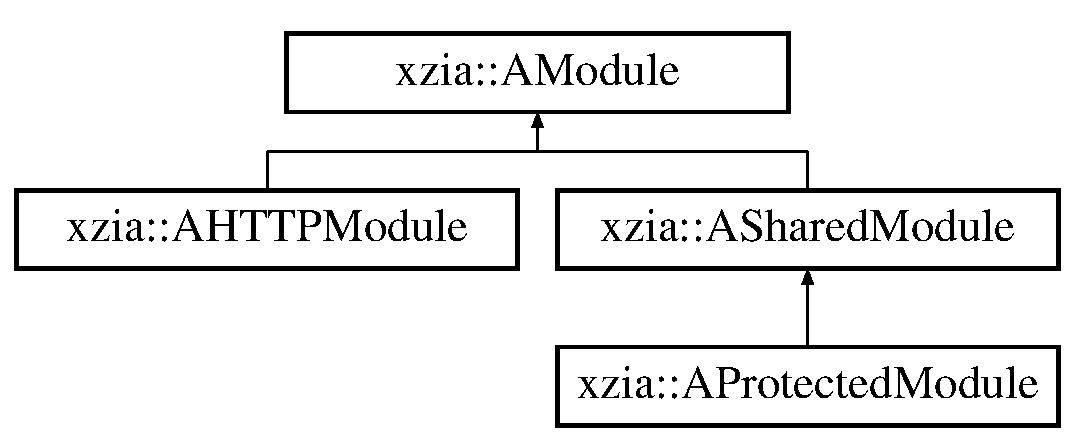
\includegraphics[height=3.000000cm]{classxzia_1_1AModule}
\end{center}
\end{figure}
\subsection*{Public Types}
\begin{DoxyCompactItemize}
\item 
enum \mbox{\hyperlink{classxzia_1_1AModule_a73967be2c863fcfdff0eef4a701df1e0}{Type}} \+: unsigned char \{ {\bfseries H\+T\+TP} = 0, 
{\bfseries S\+H\+A\+R\+ED}, 
{\bfseries P\+R\+O\+T\+E\+C\+T\+ED}
 \}
\end{DoxyCompactItemize}
\subsection*{Public Member Functions}
\begin{DoxyCompactItemize}
\item 
\mbox{\hyperlink{classxzia_1_1AModule_a1f9a69c543cb4d04be0a6d246ad0287d}{A\+Module}} ()=delete
\begin{DoxyCompactList}\small\item\em Default constructor deleted. \end{DoxyCompactList}\item 
\mbox{\Hypertarget{classxzia_1_1AModule_aa97df74e40876c19008735c741c84078}\label{classxzia_1_1AModule_aa97df74e40876c19008735c741c84078}} 
{\bfseries A\+Module} (std\+::string const \&name, \mbox{\hyperlink{classxzia_1_1AModuleManager}{A\+Module\+Manager}} \&module\+Manager, \mbox{\hyperlink{classxzia_1_1AModule_a73967be2c863fcfdff0eef4a701df1e0}{A\+Module\+::\+Type}} type)
\item 
\mbox{\hyperlink{classxzia_1_1AModule_a73967be2c863fcfdff0eef4a701df1e0}{Type}} \mbox{\hyperlink{classxzia_1_1AModule_ae07019977cab27aebdc34c98de35a3c8}{get\+Type}} () const
\begin{DoxyCompactList}\small\item\em Get the module type. \end{DoxyCompactList}\item 
const std\+::string \& \mbox{\hyperlink{classxzia_1_1AModule_ad948424683268c572aba3a410288ca22}{get\+Name}} () const
\begin{DoxyCompactList}\small\item\em Get the module name. \end{DoxyCompactList}\end{DoxyCompactItemize}
\subsection*{Protected Attributes}
\begin{DoxyCompactItemize}
\item 
\mbox{\Hypertarget{classxzia_1_1AModule_a6ee180b2e689fee0742b73af1e394340}\label{classxzia_1_1AModule_a6ee180b2e689fee0742b73af1e394340}} 
std\+::string {\bfseries name}
\item 
\mbox{\Hypertarget{classxzia_1_1AModule_af621d54793ce30445f164c5787acd541}\label{classxzia_1_1AModule_af621d54793ce30445f164c5787acd541}} 
\mbox{\hyperlink{classxzia_1_1AModuleManager}{A\+Module\+Manager}} \& {\bfseries module\+Manager}
\item 
\mbox{\Hypertarget{classxzia_1_1AModule_a331fe5174181857d396fe02e7e945b30}\label{classxzia_1_1AModule_a331fe5174181857d396fe02e7e945b30}} 
\mbox{\hyperlink{classxzia_1_1AModule_a73967be2c863fcfdff0eef4a701df1e0}{Type}} {\bfseries type}
\end{DoxyCompactItemize}
\subsection*{Friends}
\begin{DoxyCompactItemize}
\item 
\mbox{\Hypertarget{classxzia_1_1AModule_ad01ad146398700af5694cc756b1b1c63}\label{classxzia_1_1AModule_ad01ad146398700af5694cc756b1b1c63}} 
class {\bfseries A\+H\+T\+T\+P\+Module}
\item 
\mbox{\Hypertarget{classxzia_1_1AModule_a4be1d2f00a5bbd45249ec22d62f1ff45}\label{classxzia_1_1AModule_a4be1d2f00a5bbd45249ec22d62f1ff45}} 
class {\bfseries A\+Shared\+Module}
\end{DoxyCompactItemize}


\subsection{Member Enumeration Documentation}
\mbox{\Hypertarget{classxzia_1_1AModule_a73967be2c863fcfdff0eef4a701df1e0}\label{classxzia_1_1AModule_a73967be2c863fcfdff0eef4a701df1e0}} 
\index{xzia\+::\+A\+Module@{xzia\+::\+A\+Module}!Type@{Type}}
\index{Type@{Type}!xzia\+::\+A\+Module@{xzia\+::\+A\+Module}}
\subsubsection{\texorpdfstring{Type}{Type}}
{\footnotesize\ttfamily enum \mbox{\hyperlink{classxzia_1_1AModule_a73967be2c863fcfdff0eef4a701df1e0}{xzia\+::\+A\+Module\+::\+Type}} \+: unsigned char\hspace{0.3cm}{\ttfamily [strong]}}

of the module 

\subsection{Constructor \& Destructor Documentation}
\mbox{\Hypertarget{classxzia_1_1AModule_a1f9a69c543cb4d04be0a6d246ad0287d}\label{classxzia_1_1AModule_a1f9a69c543cb4d04be0a6d246ad0287d}} 
\index{xzia\+::\+A\+Module@{xzia\+::\+A\+Module}!A\+Module@{A\+Module}}
\index{A\+Module@{A\+Module}!xzia\+::\+A\+Module@{xzia\+::\+A\+Module}}
\subsubsection{\texorpdfstring{A\+Module()}{AModule()}}
{\footnotesize\ttfamily A\+Module\+::\+A\+Module (\begin{DoxyParamCaption}{ }\end{DoxyParamCaption})\hspace{0.3cm}{\ttfamily [delete]}}



Default constructor deleted. 

Constructor of \mbox{\hyperlink{classxzia_1_1AModule}{A\+Module}}.


\begin{DoxyParams}{Parameters}
{\em name} & Module name \\
\hline
{\em module\+Manager} & allows the module to access shared modules or modify the task execution list \\
\hline
{\em type} & Module type \\
\hline
\end{DoxyParams}


\subsection{Member Function Documentation}
\mbox{\Hypertarget{classxzia_1_1AModule_ad948424683268c572aba3a410288ca22}\label{classxzia_1_1AModule_ad948424683268c572aba3a410288ca22}} 
\index{xzia\+::\+A\+Module@{xzia\+::\+A\+Module}!get\+Name@{get\+Name}}
\index{get\+Name@{get\+Name}!xzia\+::\+A\+Module@{xzia\+::\+A\+Module}}
\subsubsection{\texorpdfstring{get\+Name()}{getName()}}
{\footnotesize\ttfamily A\+Module\+::get\+Name (\begin{DoxyParamCaption}{ }\end{DoxyParamCaption}) const}



Get the module name. 

\begin{DoxyReturn}{Returns}
Return the module name 
\end{DoxyReturn}
\mbox{\Hypertarget{classxzia_1_1AModule_ae07019977cab27aebdc34c98de35a3c8}\label{classxzia_1_1AModule_ae07019977cab27aebdc34c98de35a3c8}} 
\index{xzia\+::\+A\+Module@{xzia\+::\+A\+Module}!get\+Type@{get\+Type}}
\index{get\+Type@{get\+Type}!xzia\+::\+A\+Module@{xzia\+::\+A\+Module}}
\subsubsection{\texorpdfstring{get\+Type()}{getType()}}
{\footnotesize\ttfamily A\+Module\+::get\+Type (\begin{DoxyParamCaption}{ }\end{DoxyParamCaption}) const}



Get the module type. 

\begin{DoxyReturn}{Returns}
Return the module type 
\end{DoxyReturn}


The documentation for this class was generated from the following files\+:\begin{DoxyCompactItemize}
\item 
/home/edouard/\+Documents/2017/\+Z\+I\+A/\+Existen\+Z\+I\+A/\+A\+P\+I/include/modules/\mbox{\hyperlink{AModule_8hpp}{A\+Module.\+hpp}}\item 
/home/edouard/\+Documents/2017/\+Z\+I\+A/\+Existen\+Z\+I\+A/\+A\+P\+I/src/modules/A\+Module.\+cpp\end{DoxyCompactItemize}

\hypertarget{classAModuleManager}{}\section{A\+Module\+Manager Class Reference}
\label{classAModuleManager}\index{A\+Module\+Manager@{A\+Module\+Manager}}


The documentation for this class was generated from the following file\+:\begin{DoxyCompactItemize}
\item 
/home/edouard/\+Documents/2017/\+Z\+I\+A/\+Existen\+Z\+I\+A/\+A\+P\+I/include/modules/\mbox{\hyperlink{AModuleManager_8hpp}{A\+Module\+Manager.\+hpp}}\end{DoxyCompactItemize}

\hypertarget{classxzia_1_1AModuleManager}{}\section{xzia\+:\+:A\+Module\+Manager Class Reference}
\label{classxzia_1_1AModuleManager}\index{xzia\+::\+A\+Module\+Manager@{xzia\+::\+A\+Module\+Manager}}
Inheritance diagram for xzia\+:\+:A\+Module\+Manager\+:\begin{figure}[H]
\begin{center}
\leavevmode
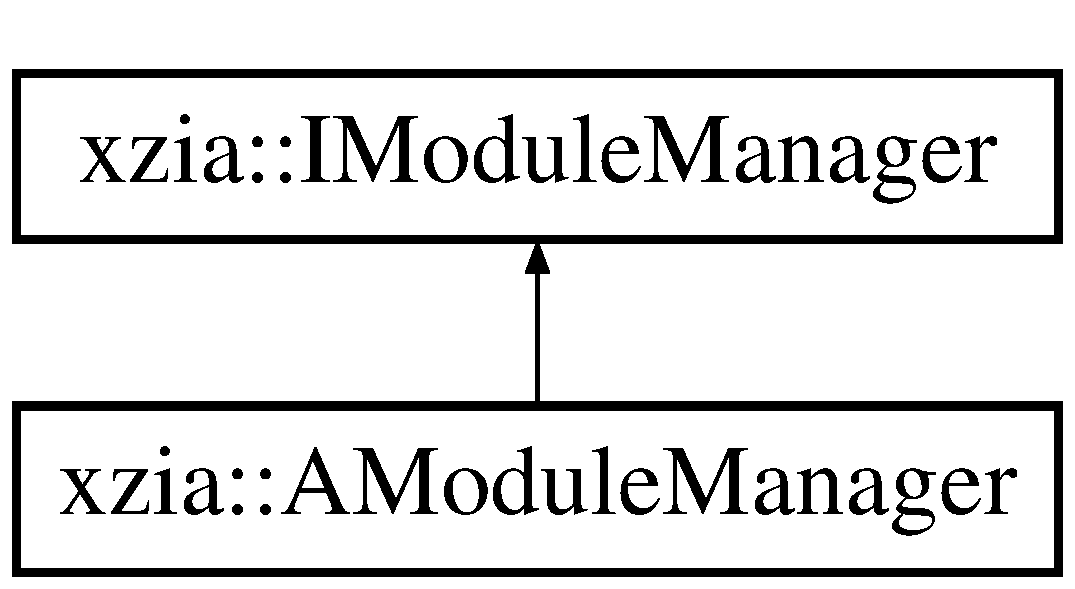
\includegraphics[height=2.000000cm]{classxzia_1_1AModuleManager}
\end{center}
\end{figure}
\subsection*{Public Member Functions}
\begin{DoxyCompactItemize}
\item 
\mbox{\hyperlink{classxzia_1_1AModuleManager_a5ef097141f352c182a661ccd620ae270}{A\+Module\+Manager}} (\mbox{\hyperlink{classxzia_1_1ALoader}{A\+Loader}} \&load)
\begin{DoxyCompactList}\small\item\em Constructor of the class \mbox{\hyperlink{classxzia_1_1AModuleManager}{A\+Module\+Manager}}. \end{DoxyCompactList}\end{DoxyCompactItemize}


\subsection{Constructor \& Destructor Documentation}
\mbox{\Hypertarget{classxzia_1_1AModuleManager_a5ef097141f352c182a661ccd620ae270}\label{classxzia_1_1AModuleManager_a5ef097141f352c182a661ccd620ae270}} 
\index{xzia\+::\+A\+Module\+Manager@{xzia\+::\+A\+Module\+Manager}!A\+Module\+Manager@{A\+Module\+Manager}}
\index{A\+Module\+Manager@{A\+Module\+Manager}!xzia\+::\+A\+Module\+Manager@{xzia\+::\+A\+Module\+Manager}}
\subsubsection{\texorpdfstring{A\+Module\+Manager()}{AModuleManager()}}
{\footnotesize\ttfamily A\+Module\+Manager\+::\+A\+Module\+Manager (\begin{DoxyParamCaption}\item[{\mbox{\hyperlink{classxzia_1_1ALoader}{xzia\+::\+A\+Loader}} \&}]{load }\end{DoxyParamCaption})\hspace{0.3cm}{\ttfamily [explicit]}}



Constructor of the class \mbox{\hyperlink{classxzia_1_1AModuleManager}{A\+Module\+Manager}}. 


\begin{DoxyParams}{Parameters}
{\em load} & Set the loader in the class \\
\hline
\end{DoxyParams}


The documentation for this class was generated from the following files\+:\begin{DoxyCompactItemize}
\item 
/home/edouard/\+Documents/2017/\+Z\+I\+A/\+Existen\+Z\+I\+A/\+A\+P\+I/include/modules/\mbox{\hyperlink{AModuleManager_8hpp}{A\+Module\+Manager.\+hpp}}\item 
/home/edouard/\+Documents/2017/\+Z\+I\+A/\+Existen\+Z\+I\+A/\+A\+P\+I/src/modules/A\+Module\+Manager.\+cpp\end{DoxyCompactItemize}

\hypertarget{classAProtectedModule}{}\section{A\+Protected\+Module Class Reference}
\label{classAProtectedModule}\index{A\+Protected\+Module@{A\+Protected\+Module}}


The documentation for this class was generated from the following file\+:\begin{DoxyCompactItemize}
\item 
/home/edouard/\+Documents/2017/\+Z\+I\+A/\+Existen\+Z\+I\+A/\+A\+P\+I/include/modules/\mbox{\hyperlink{ASharedModule_8hpp}{A\+Shared\+Module.\+hpp}}\end{DoxyCompactItemize}

\hypertarget{classxzia_1_1AProtectedModule}{}\section{xzia\+:\+:A\+Protected\+Module Class Reference}
\label{classxzia_1_1AProtectedModule}\index{xzia\+::\+A\+Protected\+Module@{xzia\+::\+A\+Protected\+Module}}
Inheritance diagram for xzia\+:\+:A\+Protected\+Module\+:\begin{figure}[H]
\begin{center}
\leavevmode
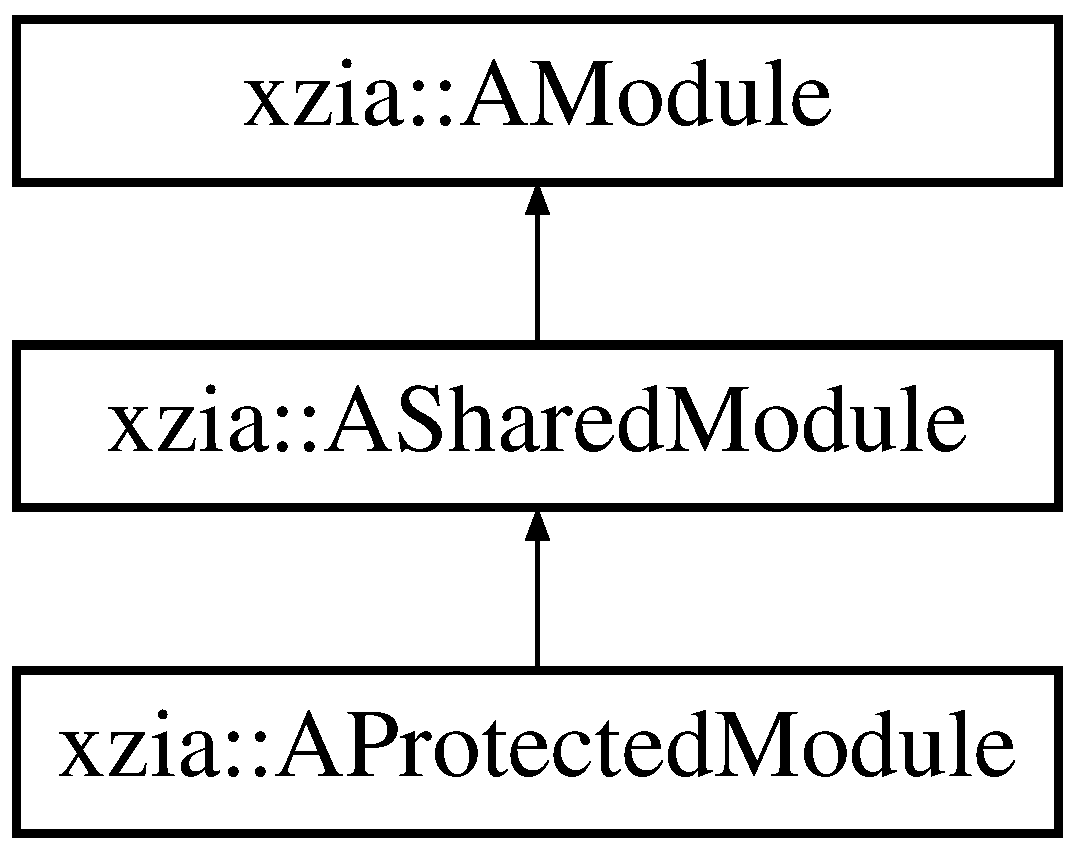
\includegraphics[height=3.000000cm]{classxzia_1_1AProtectedModule}
\end{center}
\end{figure}
\subsection*{Public Member Functions}
\begin{DoxyCompactItemize}
\item 
\mbox{\Hypertarget{classxzia_1_1AProtectedModule_acc2cf8c7c9e47bc6eafbfc8bc3d91c81}\label{classxzia_1_1AProtectedModule_acc2cf8c7c9e47bc6eafbfc8bc3d91c81}} 
{\bfseries A\+Protected\+Module} (std\+::string const \&name, \mbox{\hyperlink{classxzia_1_1AModuleManager}{A\+Module\+Manager}} \&module\+Manager)
\item 
\mbox{\hyperlink{Step_8hpp_a58ad1bb906913f90b95697c49f198770}{Step}} \mbox{\hyperlink{classxzia_1_1AProtectedModule_af8724b0d37b80ed8799c9f6b31dcdc2f}{process}} (\mbox{\hyperlink{classxzia_1_1DataStore}{Data\+Store}} \&data\+Store) final
\begin{DoxyCompactList}\small\item\em This method can be called at anytime by any module, it passes arguments through the \mbox{\hyperlink{classxzia_1_1DataStore}{Data\+Store}}. \end{DoxyCompactList}\item 
\mbox{\Hypertarget{classxzia_1_1AProtectedModule_a1959fcfb7fdd00910388293af61a84d6}\label{classxzia_1_1AProtectedModule_a1959fcfb7fdd00910388293af61a84d6}} 
{\bfseries A\+Protected\+Module} (\mbox{\hyperlink{classxzia_1_1AProtectedModule}{A\+Protected\+Module}} const \&)=delete
\item 
\mbox{\Hypertarget{classxzia_1_1AProtectedModule_a41aa7b1da39e31b13eaf0154bcc660f3}\label{classxzia_1_1AProtectedModule_a41aa7b1da39e31b13eaf0154bcc660f3}} 
{\bfseries A\+Protected\+Module} (\mbox{\hyperlink{classxzia_1_1AProtectedModule}{A\+Protected\+Module}} \&\&)=delete
\item 
\mbox{\Hypertarget{classxzia_1_1AProtectedModule_a379d8910a3eba6a36b11ef27b45fd64a}\label{classxzia_1_1AProtectedModule_a379d8910a3eba6a36b11ef27b45fd64a}} 
\mbox{\hyperlink{classxzia_1_1AProtectedModule}{A\+Protected\+Module}} \& {\bfseries operator=} (\mbox{\hyperlink{classxzia_1_1AProtectedModule}{A\+Protected\+Module}} const \&)=delete
\item 
\mbox{\Hypertarget{classxzia_1_1AProtectedModule_a43094897abe3a6efc7ee3b0332bec13f}\label{classxzia_1_1AProtectedModule_a43094897abe3a6efc7ee3b0332bec13f}} 
\mbox{\hyperlink{classxzia_1_1AProtectedModule}{A\+Protected\+Module}} \& {\bfseries operator=} (\mbox{\hyperlink{classxzia_1_1AProtectedModule}{A\+Protected\+Module}} \&\&)=delete
\end{DoxyCompactItemize}
\subsection*{Protected Member Functions}
\begin{DoxyCompactItemize}
\item 
virtual \mbox{\hyperlink{Step_8hpp_a58ad1bb906913f90b95697c49f198770}{Step}} \mbox{\hyperlink{classxzia_1_1AProtectedModule_a0f4b1e0c087fb98bdab0abe1e8205be0}{safe\+Process}} (\mbox{\hyperlink{classxzia_1_1DataStore}{Data\+Store}} \&data\+Store)=0
\begin{DoxyCompactList}\small\item\em This method is called by the process method. The logic of the module shall be coded here. This method IS thread safe, but if your logic is heavy and requires only small parts to be protected, consider using a \mbox{\hyperlink{classxzia_1_1ASharedModule}{A\+Shared\+Module}}. \end{DoxyCompactList}\end{DoxyCompactItemize}
\subsection*{Additional Inherited Members}


\subsection{Member Function Documentation}
\mbox{\Hypertarget{classxzia_1_1AProtectedModule_af8724b0d37b80ed8799c9f6b31dcdc2f}\label{classxzia_1_1AProtectedModule_af8724b0d37b80ed8799c9f6b31dcdc2f}} 
\index{xzia\+::\+A\+Protected\+Module@{xzia\+::\+A\+Protected\+Module}!process@{process}}
\index{process@{process}!xzia\+::\+A\+Protected\+Module@{xzia\+::\+A\+Protected\+Module}}
\subsubsection{\texorpdfstring{process()}{process()}}
{\footnotesize\ttfamily A\+Protected\+Module\+::process (\begin{DoxyParamCaption}\item[{\mbox{\hyperlink{classxzia_1_1DataStore}{xzia\+::\+Data\+Store}} \&}]{data\+Store }\end{DoxyParamCaption})\hspace{0.3cm}{\ttfamily [final]}, {\ttfamily [virtual]}}



This method can be called at anytime by any module, it passes arguments through the \mbox{\hyperlink{classxzia_1_1DataStore}{Data\+Store}}. 


\begin{DoxyParams}{Parameters}
{\em data\+Store} & Containing data required for the execution of the protected module \\
\hline
\end{DoxyParams}
\begin{DoxyReturn}{Returns}
a Step that let the Thread\+Pool know if it can continue to the next module or stop and send a response 
\end{DoxyReturn}


Implements \mbox{\hyperlink{classxzia_1_1ASharedModule_ac836fc027900a9c0dfdec35cb034a0a4}{xzia\+::\+A\+Shared\+Module}}.

\mbox{\Hypertarget{classxzia_1_1AProtectedModule_a0f4b1e0c087fb98bdab0abe1e8205be0}\label{classxzia_1_1AProtectedModule_a0f4b1e0c087fb98bdab0abe1e8205be0}} 
\index{xzia\+::\+A\+Protected\+Module@{xzia\+::\+A\+Protected\+Module}!safe\+Process@{safe\+Process}}
\index{safe\+Process@{safe\+Process}!xzia\+::\+A\+Protected\+Module@{xzia\+::\+A\+Protected\+Module}}
\subsubsection{\texorpdfstring{safe\+Process()}{safeProcess()}}
{\footnotesize\ttfamily A\+Protected\+Module\+::safe\+Process (\begin{DoxyParamCaption}\item[{\mbox{\hyperlink{classxzia_1_1DataStore}{Data\+Store}} \&}]{data\+Store }\end{DoxyParamCaption})\hspace{0.3cm}{\ttfamily [protected]}, {\ttfamily [pure virtual]}}



This method is called by the process method. The logic of the module shall be coded here. This method IS thread safe, but if your logic is heavy and requires only small parts to be protected, consider using a \mbox{\hyperlink{classxzia_1_1ASharedModule}{A\+Shared\+Module}}. 


\begin{DoxyParams}{Parameters}
{\em data\+Store} & Containing data required for the execution of the protected module \\
\hline
\end{DoxyParams}
\begin{DoxyReturn}{Returns}
a Step that let the Thread\+Pool know if it can continue to the next module or stop and send a response 
\end{DoxyReturn}


The documentation for this class was generated from the following files\+:\begin{DoxyCompactItemize}
\item 
/home/edouard/\+Documents/2017/\+Z\+I\+A/\+Existen\+Z\+I\+A/\+A\+P\+I/include/modules/\mbox{\hyperlink{AProtectedModule_8hpp}{A\+Protected\+Module.\+hpp}}\item 
/home/edouard/\+Documents/2017/\+Z\+I\+A/\+Existen\+Z\+I\+A/\+A\+P\+I/src/modules/A\+Protected\+Module.\+cpp\end{DoxyCompactItemize}

\hypertarget{classASharedModule}{}\section{A\+Shared\+Module Class Reference}
\label{classASharedModule}\index{A\+Shared\+Module@{A\+Shared\+Module}}


The documentation for this class was generated from the following file\+:\begin{DoxyCompactItemize}
\item 
/home/edouard/\+Documents/2017/\+Z\+I\+A/\+Existen\+Z\+I\+A/\+A\+P\+I/include/modules/\mbox{\hyperlink{ASharedModule_8hpp}{A\+Shared\+Module.\+hpp}}\end{DoxyCompactItemize}

\hypertarget{classxzia_1_1ASharedModule}{}\section{xzia\+:\+:A\+Shared\+Module Class Reference}
\label{classxzia_1_1ASharedModule}\index{xzia\+::\+A\+Shared\+Module@{xzia\+::\+A\+Shared\+Module}}
Inheritance diagram for xzia\+:\+:A\+Shared\+Module\+:\begin{figure}[H]
\begin{center}
\leavevmode
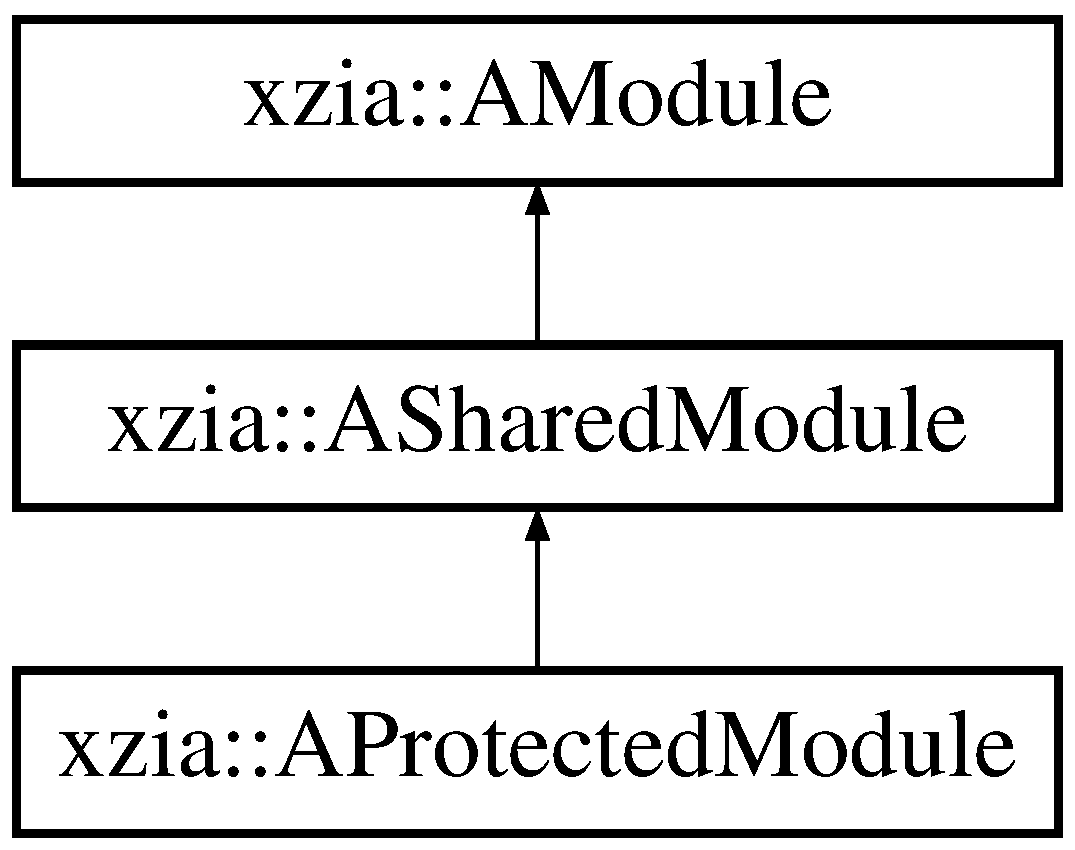
\includegraphics[height=3.000000cm]{classxzia_1_1ASharedModule}
\end{center}
\end{figure}
\subsection*{Public Member Functions}
\begin{DoxyCompactItemize}
\item 
\mbox{\Hypertarget{classxzia_1_1ASharedModule_a9bf79cf895362f8dad2075927a377311}\label{classxzia_1_1ASharedModule_a9bf79cf895362f8dad2075927a377311}} 
{\bfseries A\+Shared\+Module} (std\+::string const \&name, \mbox{\hyperlink{classxzia_1_1AModuleManager}{A\+Module\+Manager}} \&manager)
\item 
\mbox{\Hypertarget{classxzia_1_1ASharedModule_ab663fdca46a4c88594be4bc397e5a978}\label{classxzia_1_1ASharedModule_ab663fdca46a4c88594be4bc397e5a978}} 
{\bfseries A\+Shared\+Module} (std\+::string const \&name, \mbox{\hyperlink{classxzia_1_1AModuleManager}{A\+Module\+Manager}} \&manager, \mbox{\hyperlink{classxzia_1_1AModule_a73967be2c863fcfdff0eef4a701df1e0}{A\+Module\+::\+Type}} type)
\item 
virtual \mbox{\hyperlink{Step_8hpp_a58ad1bb906913f90b95697c49f198770}{Step}} \mbox{\hyperlink{classxzia_1_1ASharedModule_ac836fc027900a9c0dfdec35cb034a0a4}{process}} (\mbox{\hyperlink{classxzia_1_1DataStore}{Data\+Store}} \&data\+Store)=0
\begin{DoxyCompactList}\small\item\em This method can be called by any module that require an access to it, it passes data through the \mbox{\hyperlink{classxzia_1_1DataStore}{Data\+Store}} class. This Module is N\+OT thread safe, it is at the developer charge to protect it. \end{DoxyCompactList}\item 
\mbox{\Hypertarget{classxzia_1_1ASharedModule_a70c816fcf60d56a763d71bbfd9875738}\label{classxzia_1_1ASharedModule_a70c816fcf60d56a763d71bbfd9875738}} 
{\bfseries A\+Shared\+Module} (\mbox{\hyperlink{classxzia_1_1ASharedModule}{A\+Shared\+Module}} const \&)=delete
\item 
\mbox{\Hypertarget{classxzia_1_1ASharedModule_a990ee8fc1f178b160742a1d065ee65e5}\label{classxzia_1_1ASharedModule_a990ee8fc1f178b160742a1d065ee65e5}} 
{\bfseries A\+Shared\+Module} (\mbox{\hyperlink{classxzia_1_1ASharedModule}{A\+Shared\+Module}} \&\&)=delete
\item 
\mbox{\Hypertarget{classxzia_1_1ASharedModule_ad928b46779ce21e4d583f8245d736560}\label{classxzia_1_1ASharedModule_ad928b46779ce21e4d583f8245d736560}} 
\mbox{\hyperlink{classxzia_1_1ASharedModule}{A\+Shared\+Module}} \& {\bfseries operator=} (\mbox{\hyperlink{classxzia_1_1ASharedModule}{A\+Shared\+Module}} const \&)=delete
\item 
\mbox{\Hypertarget{classxzia_1_1ASharedModule_adc2fc36b022abe037846e3e854707d5b}\label{classxzia_1_1ASharedModule_adc2fc36b022abe037846e3e854707d5b}} 
\mbox{\hyperlink{classxzia_1_1ASharedModule}{A\+Shared\+Module}} \& {\bfseries operator=} (\mbox{\hyperlink{classxzia_1_1ASharedModule}{A\+Shared\+Module}} \&\&)=delete
\end{DoxyCompactItemize}
\subsection*{Protected Attributes}
\begin{DoxyCompactItemize}
\item 
\mbox{\Hypertarget{classxzia_1_1ASharedModule_a72f3b1b415d80fa6fc644180815ba6ef}\label{classxzia_1_1ASharedModule_a72f3b1b415d80fa6fc644180815ba6ef}} 
std\+::mutex {\bfseries mutex}
\end{DoxyCompactItemize}
\subsection*{Additional Inherited Members}


\subsection{Member Function Documentation}
\mbox{\Hypertarget{classxzia_1_1ASharedModule_ac836fc027900a9c0dfdec35cb034a0a4}\label{classxzia_1_1ASharedModule_ac836fc027900a9c0dfdec35cb034a0a4}} 
\index{xzia\+::\+A\+Shared\+Module@{xzia\+::\+A\+Shared\+Module}!process@{process}}
\index{process@{process}!xzia\+::\+A\+Shared\+Module@{xzia\+::\+A\+Shared\+Module}}
\subsubsection{\texorpdfstring{process()}{process()}}
{\footnotesize\ttfamily A\+Shared\+Module\+::process (\begin{DoxyParamCaption}\item[{\mbox{\hyperlink{classxzia_1_1DataStore}{Data\+Store}} \&}]{data\+Store }\end{DoxyParamCaption})\hspace{0.3cm}{\ttfamily [pure virtual]}}



This method can be called by any module that require an access to it, it passes data through the \mbox{\hyperlink{classxzia_1_1DataStore}{Data\+Store}} class. This Module is N\+OT thread safe, it is at the developer charge to protect it. 


\begin{DoxyParams}{Parameters}
{\em data\+Store} & \\
\hline
\end{DoxyParams}
\begin{DoxyReturn}{Returns}

\end{DoxyReturn}


Implemented in \mbox{\hyperlink{classxzia_1_1AProtectedModule_af8724b0d37b80ed8799c9f6b31dcdc2f}{xzia\+::\+A\+Protected\+Module}}.



The documentation for this class was generated from the following files\+:\begin{DoxyCompactItemize}
\item 
/home/edouard/\+Documents/2017/\+Z\+I\+A/\+Existen\+Z\+I\+A/\+A\+P\+I/include/modules/\mbox{\hyperlink{ASharedModule_8hpp}{A\+Shared\+Module.\+hpp}}\item 
/home/edouard/\+Documents/2017/\+Z\+I\+A/\+Existen\+Z\+I\+A/\+A\+P\+I/src/modules/A\+Shared\+Module.\+cpp\end{DoxyCompactItemize}

\hypertarget{classxzia_1_1ATask}{}\section{xzia\+:\+:A\+Task Class Reference}
\label{classxzia_1_1ATask}\index{xzia\+::\+A\+Task@{xzia\+::\+A\+Task}}
Inheritance diagram for xzia\+:\+:A\+Task\+:\begin{figure}[H]
\begin{center}
\leavevmode
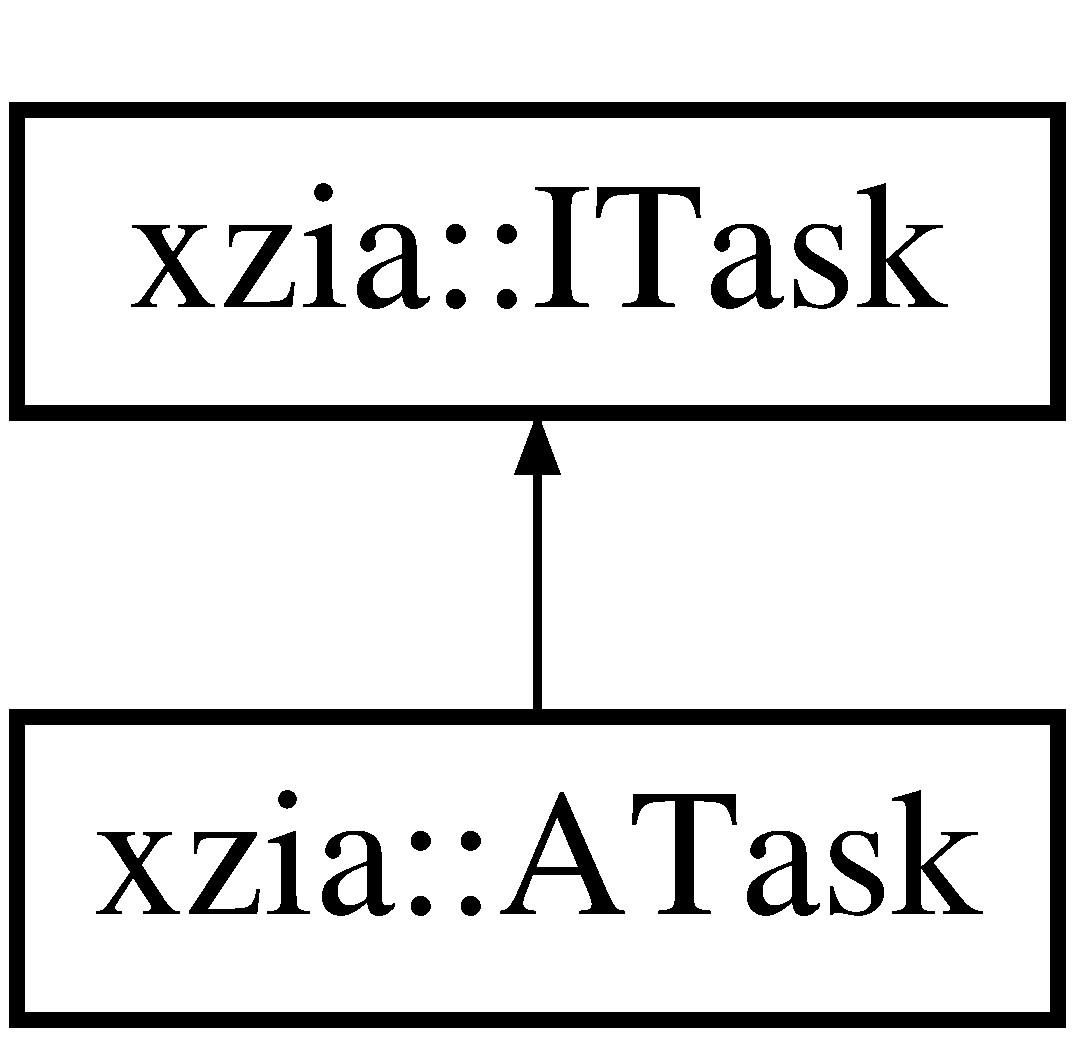
\includegraphics[height=2.000000cm]{classxzia_1_1ATask}
\end{center}
\end{figure}
\subsection*{Public Member Functions}
\begin{DoxyCompactItemize}
\item 
\mbox{\Hypertarget{classxzia_1_1ATask_a5c416483d4d81763f66c03977554e248}\label{classxzia_1_1ATask_a5c416483d4d81763f66c03977554e248}} 
{\bfseries A\+Task} (std\+::unique\+\_\+ptr$<$ \mbox{\hyperlink{structxzia_1_1Request}{Request}} $>$ req, \mbox{\hyperlink{structClient}{Client}} \&client, std\+::vector$<$ std\+::unique\+\_\+ptr$<$ \mbox{\hyperlink{classxzia_1_1AHTTPModule}{A\+H\+T\+T\+P\+Module}} $>$$>$ execution\+List)
\end{DoxyCompactItemize}
\subsection*{Protected Attributes}
\begin{DoxyCompactItemize}
\item 
\mbox{\Hypertarget{classxzia_1_1ATask_a5ac92f779f43dcc9fef86687363760b7}\label{classxzia_1_1ATask_a5ac92f779f43dcc9fef86687363760b7}} 
std\+::unique\+\_\+ptr$<$ \mbox{\hyperlink{structxzia_1_1Request}{Request}} $>$ {\bfseries req}
\item 
\mbox{\Hypertarget{classxzia_1_1ATask_a9148283ddbcf712e6ab58afb96f3c221}\label{classxzia_1_1ATask_a9148283ddbcf712e6ab58afb96f3c221}} 
\mbox{\hyperlink{structClient}{Client}} const {\bfseries client}
\item 
\mbox{\Hypertarget{classxzia_1_1ATask_ac8c8f0f62792705d3e699443e1c8771c}\label{classxzia_1_1ATask_ac8c8f0f62792705d3e699443e1c8771c}} 
std\+::vector$<$ std\+::unique\+\_\+ptr$<$ \mbox{\hyperlink{classxzia_1_1AHTTPModule}{A\+H\+T\+T\+P\+Module}} $>$ $>$ {\bfseries execution\+List}
\item 
\mbox{\Hypertarget{classxzia_1_1ATask_a65180c95061234e32d42d7313e241a28}\label{classxzia_1_1ATask_a65180c95061234e32d42d7313e241a28}} 
\mbox{\hyperlink{structxzia_1_1Response}{Response}} {\bfseries res}
\end{DoxyCompactItemize}


The documentation for this class was generated from the following file\+:\begin{DoxyCompactItemize}
\item 
/home/edouard/\+Documents/2017/\+Z\+I\+A/\+Existen\+Z\+I\+A/\+A\+P\+I/include/task/\mbox{\hyperlink{ATask_8hpp}{A\+Task.\+hpp}}\end{DoxyCompactItemize}

\hypertarget{classATask}{}\section{A\+Task Class Reference}
\label{classATask}\index{A\+Task@{A\+Task}}


The documentation for this class was generated from the following file\+:\begin{DoxyCompactItemize}
\item 
/home/edouard/\+Documents/2017/\+Z\+I\+A/\+Existen\+Z\+I\+A/\+A\+P\+I/include/task/\mbox{\hyperlink{ATask_8hpp}{A\+Task.\+hpp}}\end{DoxyCompactItemize}

\hypertarget{classxzia_1_1ATaskFactory}{}\section{xzia\+:\+:A\+Task\+Factory Class Reference}
\label{classxzia_1_1ATaskFactory}\index{xzia\+::\+A\+Task\+Factory@{xzia\+::\+A\+Task\+Factory}}
Inheritance diagram for xzia\+:\+:A\+Task\+Factory\+:\begin{figure}[H]
\begin{center}
\leavevmode
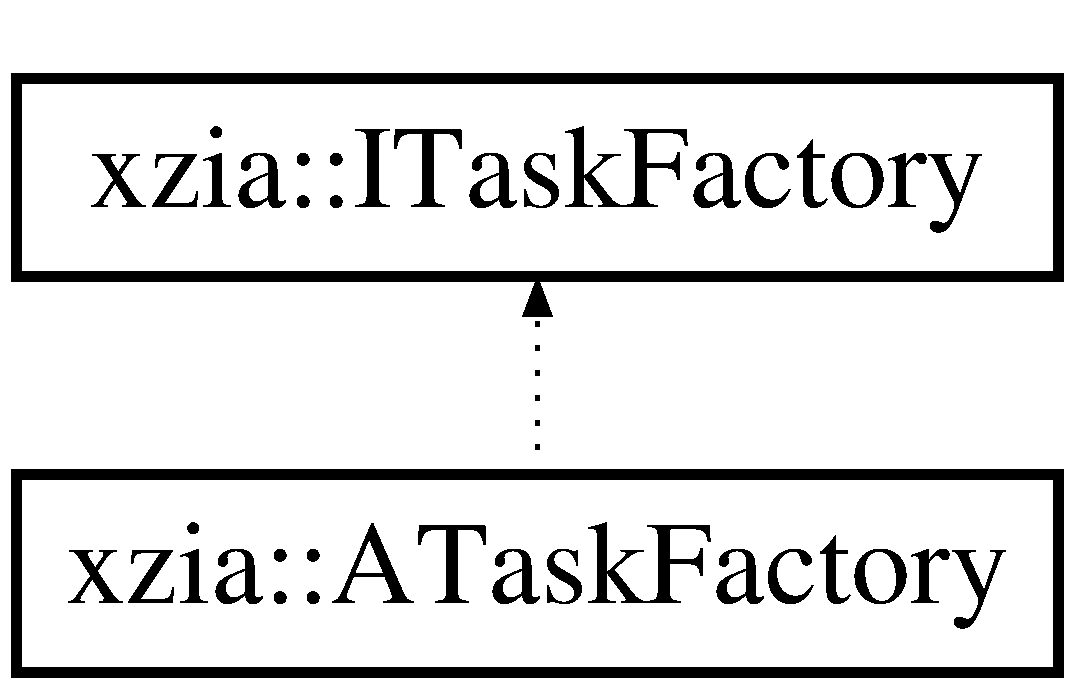
\includegraphics[height=2.000000cm]{classxzia_1_1ATaskFactory}
\end{center}
\end{figure}
\subsection*{Public Member Functions}
\begin{DoxyCompactItemize}
\item 
\mbox{\Hypertarget{classxzia_1_1ATaskFactory_a0c44c3f9e859ff8b297a31a3d240b20b}\label{classxzia_1_1ATaskFactory_a0c44c3f9e859ff8b297a31a3d240b20b}} 
{\bfseries A\+Task\+Factory} (\mbox{\hyperlink{classxzia_1_1AModuleManager}{A\+Module\+Manager}} const \&module\+Manager)
\end{DoxyCompactItemize}
\subsection*{Protected Attributes}
\begin{DoxyCompactItemize}
\item 
\mbox{\Hypertarget{classxzia_1_1ATaskFactory_a5746d8b145c2911231bc13c88b7484c4}\label{classxzia_1_1ATaskFactory_a5746d8b145c2911231bc13c88b7484c4}} 
\mbox{\hyperlink{classxzia_1_1AModuleManager}{A\+Module\+Manager}} const  \& {\bfseries module\+Manager}
\end{DoxyCompactItemize}


The documentation for this class was generated from the following files\+:\begin{DoxyCompactItemize}
\item 
/home/edouard/\+Documents/2017/\+Z\+I\+A/\+Existen\+Z\+I\+A/\+A\+P\+I/include/task/A\+Task\+Factory.\+hpp\item 
/home/edouard/\+Documents/2017/\+Z\+I\+A/\+Existen\+Z\+I\+A/\+A\+P\+I/src/task/A\+Task\+Factory.\+cpp\end{DoxyCompactItemize}

\hypertarget{classATaskFactory}{}\section{A\+Task\+Factory Class Reference}
\label{classATaskFactory}\index{A\+Task\+Factory@{A\+Task\+Factory}}


The documentation for this class was generated from the following file\+:\begin{DoxyCompactItemize}
\item 
/home/edouard/\+Documents/2017/\+Z\+I\+A/\+Existen\+Z\+I\+A/\+A\+P\+I/include/task/\mbox{\hyperlink{ATaskFactory_8hpp}{A\+Task\+Factory.\+hpp}}\end{DoxyCompactItemize}

\hypertarget{classAThreadPool}{}\section{A\+Thread\+Pool Class Reference}
\label{classAThreadPool}\index{A\+Thread\+Pool@{A\+Thread\+Pool}}


The documentation for this class was generated from the following file\+:\begin{DoxyCompactItemize}
\item 
/home/edouard/\+Documents/2017/\+Z\+I\+A/\+Existen\+Z\+I\+A/\+A\+P\+I/include/thread/\mbox{\hyperlink{AThreadPool_8hpp}{A\+Thread\+Pool.\+hpp}}\end{DoxyCompactItemize}

\hypertarget{classxzia_1_1AThreadPool}{}\section{xzia\+:\+:A\+Thread\+Pool Class Reference}
\label{classxzia_1_1AThreadPool}\index{xzia\+::\+A\+Thread\+Pool@{xzia\+::\+A\+Thread\+Pool}}
Inheritance diagram for xzia\+:\+:A\+Thread\+Pool\+:\begin{figure}[H]
\begin{center}
\leavevmode
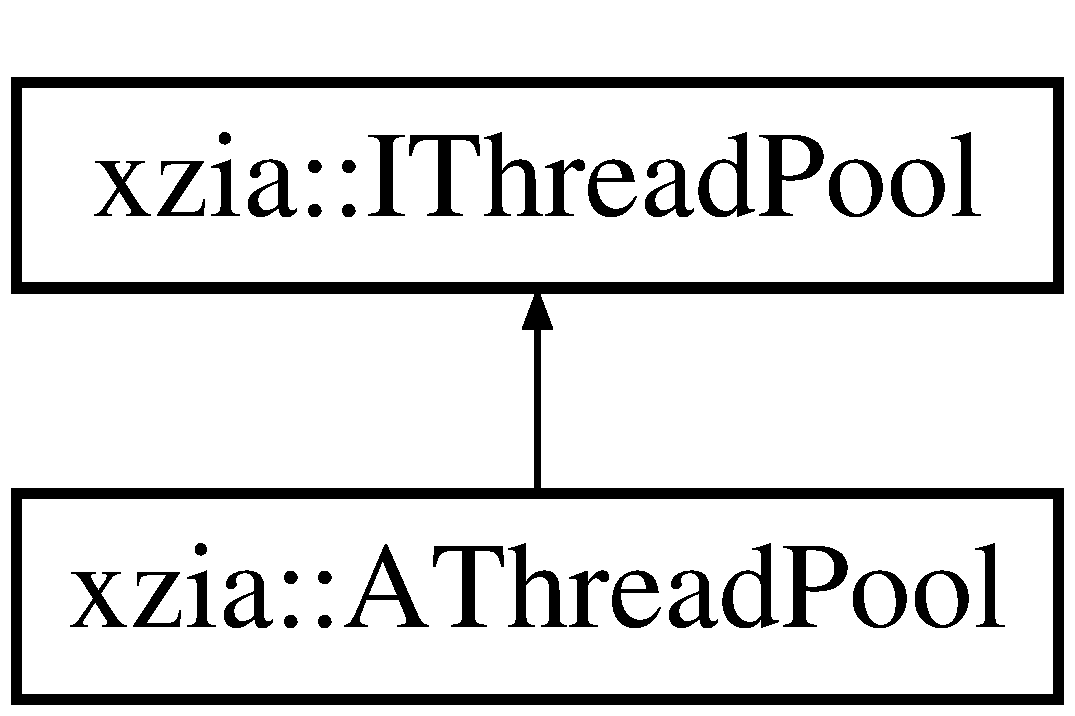
\includegraphics[height=2.000000cm]{classxzia_1_1AThreadPool}
\end{center}
\end{figure}
\subsection*{Public Member Functions}
\begin{DoxyCompactItemize}
\item 
\mbox{\Hypertarget{classxzia_1_1AThreadPool_ab35fcbd9ff967ca953140c1f69d3ff02}\label{classxzia_1_1AThreadPool_ab35fcbd9ff967ca953140c1f69d3ff02}} 
{\bfseries A\+Thread\+Pool} (unsigned int nb\+Threads)
\end{DoxyCompactItemize}
\subsection*{Protected Member Functions}
\begin{DoxyCompactItemize}
\item 
virtual void \mbox{\hyperlink{classxzia_1_1AThreadPool_a6c5378fecadb2043b50091f3995dc785}{thread\+Workflow}} (unsigned int id)=0
\begin{DoxyCompactList}\small\item\em Method which launch a thread with a given id. \end{DoxyCompactList}\end{DoxyCompactItemize}
\subsection*{Protected Attributes}
\begin{DoxyCompactItemize}
\item 
\mbox{\Hypertarget{classxzia_1_1AThreadPool_ab73a7a7d0a1530157c318122c8a819fa}\label{classxzia_1_1AThreadPool_ab73a7a7d0a1530157c318122c8a819fa}} 
std\+::vector$<$ std\+::thread $>$ {\bfseries threads}
\item 
\mbox{\Hypertarget{classxzia_1_1AThreadPool_a01d8dc990cd888ded9e951c0e667d2e0}\label{classxzia_1_1AThreadPool_a01d8dc990cd888ded9e951c0e667d2e0}} 
std\+::queue$<$ std\+::unique\+\_\+ptr$<$ \mbox{\hyperlink{classxzia_1_1ATask}{A\+Task}} $>$ $>$ {\bfseries todo\+Tasks}
\item 
\mbox{\Hypertarget{classxzia_1_1AThreadPool_ae8f8619cb333433e2f5f54f27062e55b}\label{classxzia_1_1AThreadPool_ae8f8619cb333433e2f5f54f27062e55b}} 
std\+::queue$<$ std\+::unique\+\_\+ptr$<$ \mbox{\hyperlink{classxzia_1_1ATask}{A\+Task}} $>$ $>$ {\bfseries done\+Tasks}
\item 
\mbox{\Hypertarget{classxzia_1_1AThreadPool_ad1c6a821ed59000b16f73216b65df2d2}\label{classxzia_1_1AThreadPool_ad1c6a821ed59000b16f73216b65df2d2}} 
std\+::vector$<$ \mbox{\hyperlink{ThreadState_8hpp_a33f2462f9bd05760c2ce5ce111a5a97b}{Thread\+State}} $>$ {\bfseries state}
\item 
\mbox{\Hypertarget{classxzia_1_1AThreadPool_afe629e748ba9a5e372b005a7338e1c89}\label{classxzia_1_1AThreadPool_afe629e748ba9a5e372b005a7338e1c89}} 
std\+::atomic$<$ bool $>$ {\bfseries running}
\item 
\mbox{\Hypertarget{classxzia_1_1AThreadPool_ac790322a9a5b838c7c7171cd2280542a}\label{classxzia_1_1AThreadPool_ac790322a9a5b838c7c7171cd2280542a}} 
std\+::condition\+\_\+variable {\bfseries condvar}
\item 
\mbox{\Hypertarget{classxzia_1_1AThreadPool_a000c60518a6828d1e74a224c0a26b2b7}\label{classxzia_1_1AThreadPool_a000c60518a6828d1e74a224c0a26b2b7}} 
std\+::mutex {\bfseries mutex}
\end{DoxyCompactItemize}


\subsection{Member Function Documentation}
\mbox{\Hypertarget{classxzia_1_1AThreadPool_a6c5378fecadb2043b50091f3995dc785}\label{classxzia_1_1AThreadPool_a6c5378fecadb2043b50091f3995dc785}} 
\index{xzia\+::\+A\+Thread\+Pool@{xzia\+::\+A\+Thread\+Pool}!thread\+Workflow@{thread\+Workflow}}
\index{thread\+Workflow@{thread\+Workflow}!xzia\+::\+A\+Thread\+Pool@{xzia\+::\+A\+Thread\+Pool}}
\subsubsection{\texorpdfstring{thread\+Workflow()}{threadWorkflow()}}
{\footnotesize\ttfamily A\+Thread\+Pool\+::thread\+Workflow (\begin{DoxyParamCaption}\item[{unsigned int}]{id }\end{DoxyParamCaption})\hspace{0.3cm}{\ttfamily [protected]}, {\ttfamily [pure virtual]}}



Method which launch a thread with a given id. 


\begin{DoxyParams}{Parameters}
{\em id} & Id given to the thread \\
\hline
\end{DoxyParams}


The documentation for this class was generated from the following files\+:\begin{DoxyCompactItemize}
\item 
/home/edouard/\+Documents/2017/\+Z\+I\+A/\+Existen\+Z\+I\+A/\+A\+P\+I/include/thread/\mbox{\hyperlink{AThreadPool_8hpp}{A\+Thread\+Pool.\+hpp}}\item 
/home/edouard/\+Documents/2017/\+Z\+I\+A/\+Existen\+Z\+I\+A/\+A\+P\+I/src/thread/A\+Thread\+Pool.\+cpp\end{DoxyCompactItemize}

\hypertarget{structClient}{}\section{Client Struct Reference}
\label{structClient}\index{Client@{Client}}


The documentation for this struct was generated from the following file\+:\begin{DoxyCompactItemize}
\item 
/home/edouard/\+Documents/2017/\+Z\+I\+A/\+Existen\+Z\+I\+A/\+A\+P\+I/include/client/\mbox{\hyperlink{Client_8hpp}{Client.\+hpp}}\end{DoxyCompactItemize}

\hypertarget{classDataStore}{}\section{Data\+Store Class Reference}
\label{classDataStore}\index{Data\+Store@{Data\+Store}}


The documentation for this class was generated from the following file\+:\begin{DoxyCompactItemize}
\item 
/home/edouard/\+Documents/2017/\+Z\+I\+A/\+Existen\+Z\+I\+A/\+A\+P\+I/include/modules/\mbox{\hyperlink{DataStore_8hpp}{Data\+Store.\+hpp}}\end{DoxyCompactItemize}

\hypertarget{classxzia_1_1DataStore}{}\section{xzia\+:\+:Data\+Store Class Reference}
\label{classxzia_1_1DataStore}\index{xzia\+::\+Data\+Store@{xzia\+::\+Data\+Store}}
\subsection*{Public Member Functions}
\begin{DoxyCompactItemize}
\item 
{\footnotesize template$<$typename T $>$ }\\void \mbox{\hyperlink{classxzia_1_1DataStore_a97301fd6dfa58a88b9903fb7fdf307a1}{add\+Data}} (std\+::string const \&key, T data)
\begin{DoxyCompactList}\small\item\em Add data of any type. \end{DoxyCompactList}\item 
{\footnotesize template$<$typename T $>$ }\\T \mbox{\hyperlink{classxzia_1_1DataStore_a91fb035bfe2bebe2e21a0cf5aaad5a04}{get\+Data}} (std\+::string const \&key)
\begin{DoxyCompactList}\small\item\em Add data of type char. \end{DoxyCompactList}\end{DoxyCompactItemize}
\subsection*{Protected Attributes}
\begin{DoxyCompactItemize}
\item 
\mbox{\Hypertarget{classxzia_1_1DataStore_a3bbea48eb0a1432158a016315c3d1557}\label{classxzia_1_1DataStore_a3bbea48eb0a1432158a016315c3d1557}} 
std\+::map$<$ std\+::string, variant $>$ {\bfseries datas}
\end{DoxyCompactItemize}


\subsection{Member Function Documentation}
\mbox{\Hypertarget{classxzia_1_1DataStore_a97301fd6dfa58a88b9903fb7fdf307a1}\label{classxzia_1_1DataStore_a97301fd6dfa58a88b9903fb7fdf307a1}} 
\index{xzia\+::\+Data\+Store@{xzia\+::\+Data\+Store}!add\+Data@{add\+Data}}
\index{add\+Data@{add\+Data}!xzia\+::\+Data\+Store@{xzia\+::\+Data\+Store}}
\subsubsection{\texorpdfstring{add\+Data()}{addData()}}
{\footnotesize\ttfamily template$<$typename T $>$ \\
xzia\+::\+Data\+Store\+::add\+Data (\begin{DoxyParamCaption}\item[{std\+::string const \&}]{key,  }\item[{T}]{data }\end{DoxyParamCaption})\hspace{0.3cm}{\ttfamily [inline]}}



Add data of any type. 


\begin{DoxyParams}{Parameters}
{\em data} & Data to be added \\
\hline
{\em key} & Key associated to the data adding \\
\hline
\end{DoxyParams}
\mbox{\Hypertarget{classxzia_1_1DataStore_a91fb035bfe2bebe2e21a0cf5aaad5a04}\label{classxzia_1_1DataStore_a91fb035bfe2bebe2e21a0cf5aaad5a04}} 
\index{xzia\+::\+Data\+Store@{xzia\+::\+Data\+Store}!get\+Data@{get\+Data}}
\index{get\+Data@{get\+Data}!xzia\+::\+Data\+Store@{xzia\+::\+Data\+Store}}
\subsubsection{\texorpdfstring{get\+Data()}{getData()}}
{\footnotesize\ttfamily template$<$typename T $>$ \\
T xzia\+::\+Data\+Store\+::get\+Data (\begin{DoxyParamCaption}\item[{std\+::string const \&}]{key }\end{DoxyParamCaption})\hspace{0.3cm}{\ttfamily [inline]}}



Add data of type char. 


\begin{DoxyParams}{Parameters}
{\em c} & Data of type char \\
\hline
{\em key} & Key associated to the data adding \\
\hline
\end{DoxyParams}


The documentation for this class was generated from the following file\+:\begin{DoxyCompactItemize}
\item 
/home/edouard/\+Documents/2017/\+Z\+I\+A/\+Existen\+Z\+I\+A/\+A\+P\+I/include/modules/Data\+Store.\+hpp\end{DoxyCompactItemize}

\hypertarget{classxzia_1_1IConfigLoader}{}\section{xzia\+:\+:I\+Config\+Loader Class Reference}
\label{classxzia_1_1IConfigLoader}\index{xzia\+::\+I\+Config\+Loader@{xzia\+::\+I\+Config\+Loader}}
\subsection*{Public Member Functions}
\begin{DoxyCompactItemize}
\item 
virtual std\+::map$<$ std\+::string, std\+::string $>$ \mbox{\hyperlink{classxzia_1_1IConfigLoader_acc495c84824d91f3baf1bfdbce2d4f60}{get\+Module\+Config}} (std\+::string const \&module)=0
\begin{DoxyCompactList}\small\item\em Retrieve the configuration of a module from the loader. \end{DoxyCompactList}\item 
virtual std\+::vector$<$ std\+::string $>$ \mbox{\hyperlink{classxzia_1_1IConfigLoader_a978f88a37cacd8ad84bd3ae995e5a7ba}{get\+Execution\+List\+Model}} ()=0
\begin{DoxyCompactList}\small\item\em Retrieve the task list of modules that will processes the request received by the server. \end{DoxyCompactList}\item 
virtual std\+::map$<$ std\+::string, std\+::string $>$ \mbox{\hyperlink{classxzia_1_1IConfigLoader_a343df444ba504f635e7204445105bbef}{get\+Core\+Config}} ()=0
\begin{DoxyCompactList}\small\item\em Retrieve the configuration of the core from the loader. \end{DoxyCompactList}\end{DoxyCompactItemize}


\subsection{Member Function Documentation}
\mbox{\Hypertarget{classxzia_1_1IConfigLoader_a343df444ba504f635e7204445105bbef}\label{classxzia_1_1IConfigLoader_a343df444ba504f635e7204445105bbef}} 
\index{xzia\+::\+I\+Config\+Loader@{xzia\+::\+I\+Config\+Loader}!get\+Core\+Config@{get\+Core\+Config}}
\index{get\+Core\+Config@{get\+Core\+Config}!xzia\+::\+I\+Config\+Loader@{xzia\+::\+I\+Config\+Loader}}
\subsubsection{\texorpdfstring{get\+Core\+Config()}{getCoreConfig()}}
{\footnotesize\ttfamily I\+Config\+Loader\+::get\+Core\+Config (\begin{DoxyParamCaption}{ }\end{DoxyParamCaption})\hspace{0.3cm}{\ttfamily [pure virtual]}}



Retrieve the configuration of the core from the loader. 

\begin{DoxyReturn}{Returns}
the configuration of the core as a map 
\end{DoxyReturn}
\mbox{\Hypertarget{classxzia_1_1IConfigLoader_a978f88a37cacd8ad84bd3ae995e5a7ba}\label{classxzia_1_1IConfigLoader_a978f88a37cacd8ad84bd3ae995e5a7ba}} 
\index{xzia\+::\+I\+Config\+Loader@{xzia\+::\+I\+Config\+Loader}!get\+Execution\+List\+Model@{get\+Execution\+List\+Model}}
\index{get\+Execution\+List\+Model@{get\+Execution\+List\+Model}!xzia\+::\+I\+Config\+Loader@{xzia\+::\+I\+Config\+Loader}}
\subsubsection{\texorpdfstring{get\+Execution\+List\+Model()}{getExecutionListModel()}}
{\footnotesize\ttfamily I\+Config\+Loader\+::get\+Execution\+List\+Model (\begin{DoxyParamCaption}{ }\end{DoxyParamCaption})\hspace{0.3cm}{\ttfamily [pure virtual]}}



Retrieve the task list of modules that will processes the request received by the server. 

\begin{DoxyReturn}{Returns}
Return the name of all the modules in a vector 
\end{DoxyReturn}
\mbox{\Hypertarget{classxzia_1_1IConfigLoader_acc495c84824d91f3baf1bfdbce2d4f60}\label{classxzia_1_1IConfigLoader_acc495c84824d91f3baf1bfdbce2d4f60}} 
\index{xzia\+::\+I\+Config\+Loader@{xzia\+::\+I\+Config\+Loader}!get\+Module\+Config@{get\+Module\+Config}}
\index{get\+Module\+Config@{get\+Module\+Config}!xzia\+::\+I\+Config\+Loader@{xzia\+::\+I\+Config\+Loader}}
\subsubsection{\texorpdfstring{get\+Module\+Config()}{getModuleConfig()}}
{\footnotesize\ttfamily I\+Config\+Loader\+::get\+Module\+Config (\begin{DoxyParamCaption}\item[{std\+::string const \&}]{module }\end{DoxyParamCaption})\hspace{0.3cm}{\ttfamily [pure virtual]}}



Retrieve the configuration of a module from the loader. 


\begin{DoxyParams}{Parameters}
{\em module} & name \\
\hline
\end{DoxyParams}
\begin{DoxyReturn}{Returns}
the configuration of the module as a map 
\end{DoxyReturn}


The documentation for this class was generated from the following file\+:\begin{DoxyCompactItemize}
\item 
/home/edouard/\+Documents/2017/\+Z\+I\+A/\+Existen\+Z\+I\+A/\+A\+P\+I/include/loader/\mbox{\hyperlink{IConfigLoader_8hpp}{I\+Config\+Loader.\+hpp}}\end{DoxyCompactItemize}

\hypertarget{classIConfigLoader}{}\section{I\+Config\+Loader Class Reference}
\label{classIConfigLoader}\index{I\+Config\+Loader@{I\+Config\+Loader}}


The documentation for this class was generated from the following file\+:\begin{DoxyCompactItemize}
\item 
/home/edouard/\+Documents/2017/\+Z\+I\+A/\+Existen\+Z\+I\+A/\+A\+P\+I/include/loader/\mbox{\hyperlink{IConfigLoader_8hpp}{I\+Config\+Loader.\+hpp}}\end{DoxyCompactItemize}

\hypertarget{classxzia_1_1ICore}{}\section{xzia\+:\+:I\+Core Class Reference}
\label{classxzia_1_1ICore}\index{xzia\+::\+I\+Core@{xzia\+::\+I\+Core}}
Inheritance diagram for xzia\+:\+:I\+Core\+:\begin{figure}[H]
\begin{center}
\leavevmode
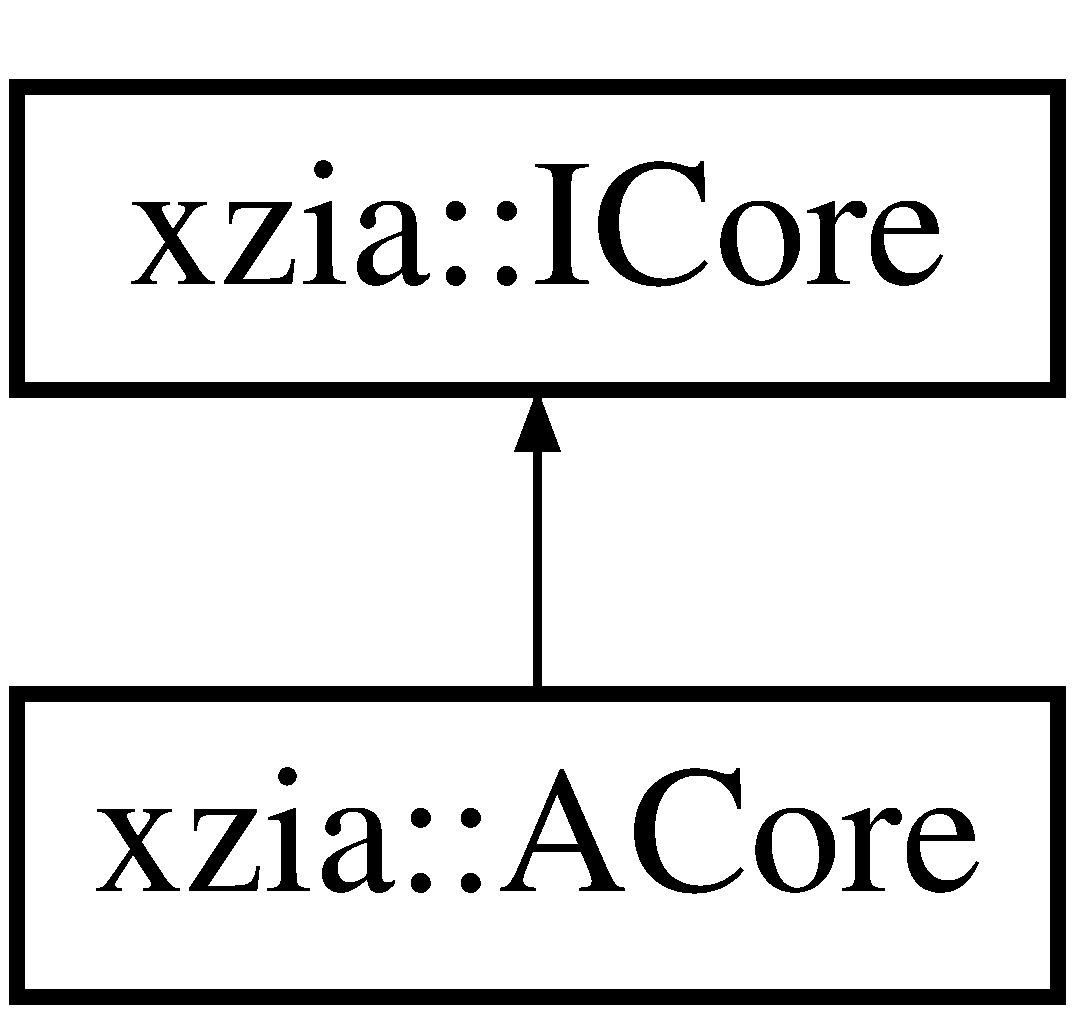
\includegraphics[height=2.000000cm]{classxzia_1_1ICore}
\end{center}
\end{figure}
\subsection*{Public Member Functions}
\begin{DoxyCompactItemize}
\item 
\mbox{\Hypertarget{classxzia_1_1ICore_a892d1d93609f5f4ea0c788f74cc9d81d}\label{classxzia_1_1ICore_a892d1d93609f5f4ea0c788f74cc9d81d}} 
virtual void \mbox{\hyperlink{classxzia_1_1ICore_a892d1d93609f5f4ea0c788f74cc9d81d}{run}} ()=0
\begin{DoxyCompactList}\small\item\em This method run the core of this A\+PI. We can adapt this method for the type of request we want to implement. \end{DoxyCompactList}\end{DoxyCompactItemize}


The documentation for this class was generated from the following file\+:\begin{DoxyCompactItemize}
\item 
/home/edouard/\+Documents/2017/\+Z\+I\+A/\+Existen\+Z\+I\+A/\+A\+P\+I/include/core/\mbox{\hyperlink{ICore_8hpp}{I\+Core.\+hpp}}\end{DoxyCompactItemize}

\hypertarget{classICore}{}\section{I\+Core Class Reference}
\label{classICore}\index{I\+Core@{I\+Core}}


The documentation for this class was generated from the following file\+:\begin{DoxyCompactItemize}
\item 
/home/edouard/\+Documents/2017/\+Z\+I\+A/\+Existen\+Z\+I\+A/\+A\+P\+I/include/core/\mbox{\hyperlink{ICore_8hpp}{I\+Core.\+hpp}}\end{DoxyCompactItemize}

\hypertarget{classxzia_1_1ILoader}{}\section{xzia\+:\+:I\+Loader Class Reference}
\label{classxzia_1_1ILoader}\index{xzia\+::\+I\+Loader@{xzia\+::\+I\+Loader}}
Inheritance diagram for xzia\+:\+:I\+Loader\+:\begin{figure}[H]
\begin{center}
\leavevmode
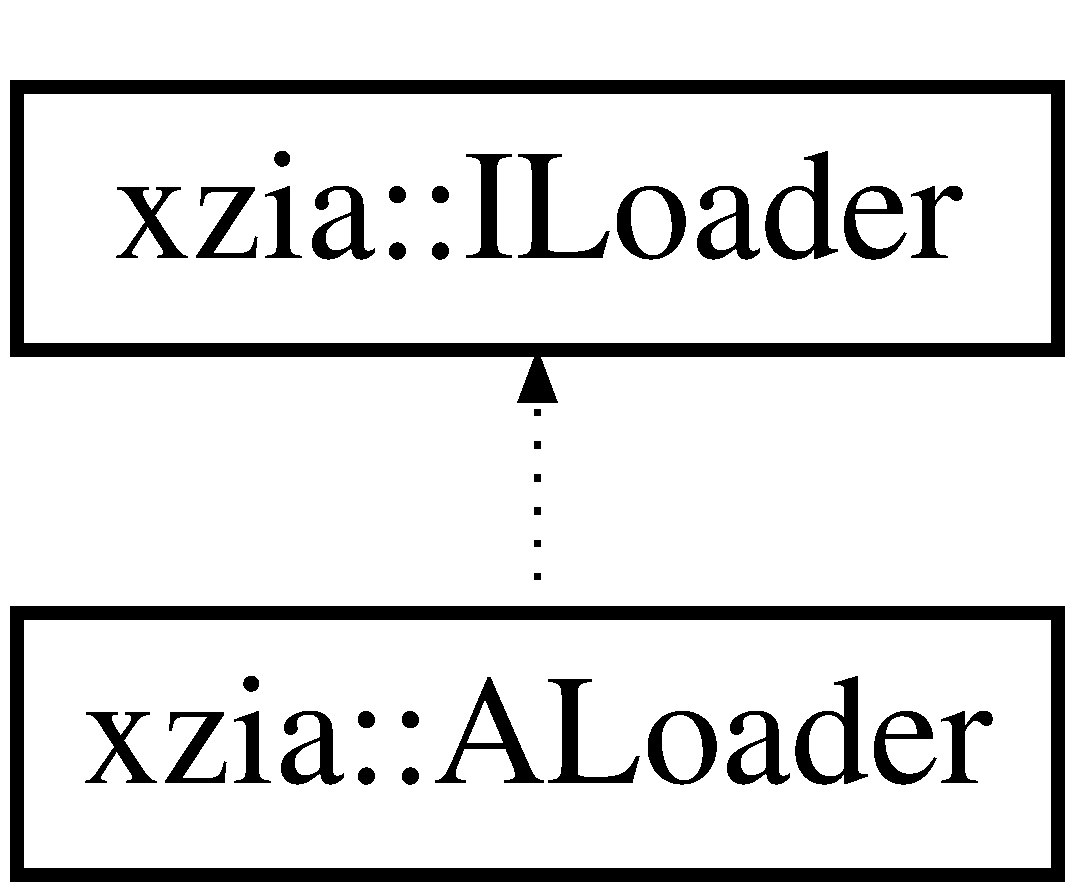
\includegraphics[height=2.000000cm]{classxzia_1_1ILoader}
\end{center}
\end{figure}
\subsection*{Public Member Functions}
\begin{DoxyCompactItemize}
\item 
\mbox{\Hypertarget{classxzia_1_1ILoader_a8662be66536e6414c223d7f4d861e7d9}\label{classxzia_1_1ILoader_a8662be66536e6414c223d7f4d861e7d9}} 
virtual void \mbox{\hyperlink{classxzia_1_1ILoader_a8662be66536e6414c223d7f4d861e7d9}{reload}} ()=0
\begin{DoxyCompactList}\small\item\em This method allows the loader to reload the configuration, updating the list of available modules, and their corresponding configuration. \end{DoxyCompactList}\item 
virtual std\+::unique\+\_\+ptr$<$ \mbox{\hyperlink{classxzia_1_1AModule}{A\+Module}} $>$ \mbox{\hyperlink{classxzia_1_1ILoader_a6aad71496e1ebfa29aebe1c351a1e871}{load\+Module}} (std\+::string const \&module)=0
\begin{DoxyCompactList}\small\item\em This method loads a module. \end{DoxyCompactList}\end{DoxyCompactItemize}


\subsection{Member Function Documentation}
\mbox{\Hypertarget{classxzia_1_1ILoader_a6aad71496e1ebfa29aebe1c351a1e871}\label{classxzia_1_1ILoader_a6aad71496e1ebfa29aebe1c351a1e871}} 
\index{xzia\+::\+I\+Loader@{xzia\+::\+I\+Loader}!load\+Module@{load\+Module}}
\index{load\+Module@{load\+Module}!xzia\+::\+I\+Loader@{xzia\+::\+I\+Loader}}
\subsubsection{\texorpdfstring{load\+Module()}{loadModule()}}
{\footnotesize\ttfamily I\+Loader\+::load\+Module (\begin{DoxyParamCaption}\item[{std\+::string const \&}]{module }\end{DoxyParamCaption})\hspace{0.3cm}{\ttfamily [pure virtual]}}



This method loads a module. 


\begin{DoxyParams}{Parameters}
{\em module} & \\
\hline
\end{DoxyParams}


The documentation for this class was generated from the following file\+:\begin{DoxyCompactItemize}
\item 
/home/edouard/\+Documents/2017/\+Z\+I\+A/\+Existen\+Z\+I\+A/\+A\+P\+I/include/loader/\mbox{\hyperlink{ILoader_8hpp}{I\+Loader.\+hpp}}\end{DoxyCompactItemize}

\hypertarget{classILoader}{}\section{I\+Loader Class Reference}
\label{classILoader}\index{I\+Loader@{I\+Loader}}


The documentation for this class was generated from the following file\+:\begin{DoxyCompactItemize}
\item 
/home/edouard/\+Documents/2017/\+Z\+I\+A/\+Existen\+Z\+I\+A/\+A\+P\+I/include/loader/\mbox{\hyperlink{ILoader_8hpp}{I\+Loader.\+hpp}}\end{DoxyCompactItemize}

\hypertarget{classIModuleManager}{}\section{I\+Module\+Manager Class Reference}
\label{classIModuleManager}\index{I\+Module\+Manager@{I\+Module\+Manager}}


The documentation for this class was generated from the following file\+:\begin{DoxyCompactItemize}
\item 
/home/edouard/\+Documents/2017/\+Z\+I\+A/\+Existen\+Z\+I\+A/\+A\+P\+I/include/modules/\mbox{\hyperlink{IModuleManager_8hpp}{I\+Module\+Manager.\+hpp}}\end{DoxyCompactItemize}

\hypertarget{classxzia_1_1IModuleManager}{}\section{xzia\+:\+:I\+Module\+Manager Class Reference}
\label{classxzia_1_1IModuleManager}\index{xzia\+::\+I\+Module\+Manager@{xzia\+::\+I\+Module\+Manager}}
Inheritance diagram for xzia\+:\+:I\+Module\+Manager\+:\begin{figure}[H]
\begin{center}
\leavevmode
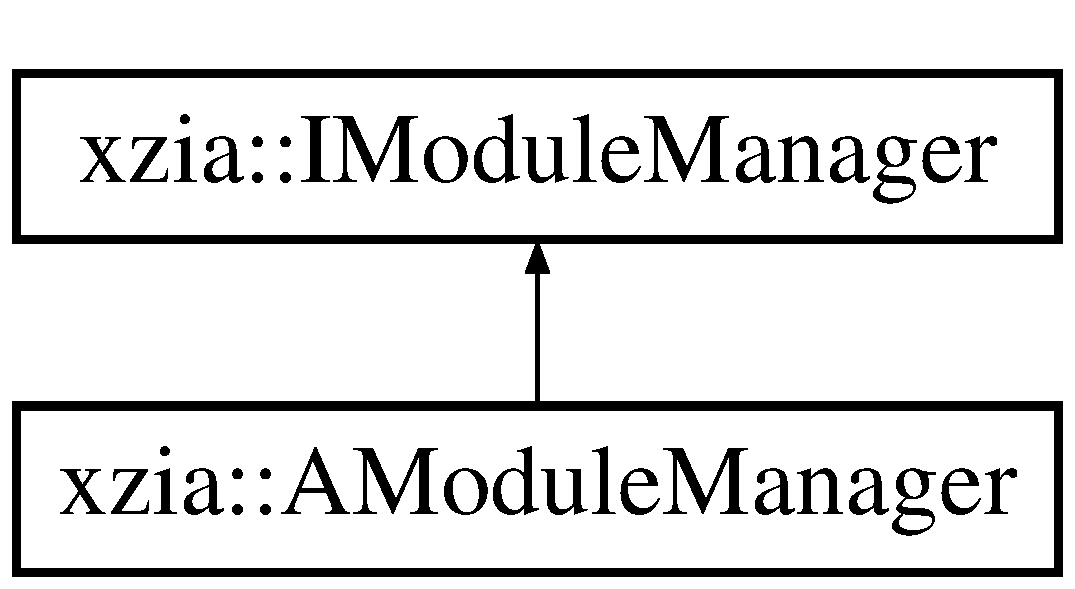
\includegraphics[height=2.000000cm]{classxzia_1_1IModuleManager}
\end{center}
\end{figure}
\subsection*{Public Member Functions}
\begin{DoxyCompactItemize}
\item 
virtual \mbox{\hyperlink{classxzia_1_1ASharedModule}{A\+Shared\+Module}} \& \mbox{\hyperlink{classxzia_1_1IModuleManager_a56addcdec0c0b32595807672705b414b}{get\+Shared\+Module}} (std\+::string const \&module)=0
\begin{DoxyCompactList}\small\item\em Shared module getter. \end{DoxyCompactList}\item 
\mbox{\Hypertarget{classxzia_1_1IModuleManager_aa255ae4721e3575c3e0a83c2bcc1549b}\label{classxzia_1_1IModuleManager_aa255ae4721e3575c3e0a83c2bcc1549b}} 
virtual std\+::unique\+\_\+ptr$<$ \mbox{\hyperlink{classxzia_1_1AHTTPModule}{A\+H\+T\+T\+P\+Module}} $>$ {\bfseries get\+H\+T\+T\+P\+Module} (std\+::string const \&module)=0
\item 
\mbox{\Hypertarget{classxzia_1_1IModuleManager_a0edf1a81440b0f76ef6b6f66cc046fe1}\label{classxzia_1_1IModuleManager_a0edf1a81440b0f76ef6b6f66cc046fe1}} 
virtual void \mbox{\hyperlink{classxzia_1_1IModuleManager_a0edf1a81440b0f76ef6b6f66cc046fe1}{reload}} ()=0
\begin{DoxyCompactList}\small\item\em Notify the module manager that modules must be reloaded. \end{DoxyCompactList}\item 
\mbox{\Hypertarget{classxzia_1_1IModuleManager_a8416910511a3434b6a140b45dd1bab13}\label{classxzia_1_1IModuleManager_a8416910511a3434b6a140b45dd1bab13}} 
virtual std\+::vector$<$ \mbox{\hyperlink{classxzia_1_1AHTTPModule}{A\+H\+T\+T\+P\+Module}} $>$ {\bfseries get\+Execution\+List\+Model} ()=0
\end{DoxyCompactItemize}


\subsection{Member Function Documentation}
\mbox{\Hypertarget{classxzia_1_1IModuleManager_a56addcdec0c0b32595807672705b414b}\label{classxzia_1_1IModuleManager_a56addcdec0c0b32595807672705b414b}} 
\index{xzia\+::\+I\+Module\+Manager@{xzia\+::\+I\+Module\+Manager}!get\+Shared\+Module@{get\+Shared\+Module}}
\index{get\+Shared\+Module@{get\+Shared\+Module}!xzia\+::\+I\+Module\+Manager@{xzia\+::\+I\+Module\+Manager}}
\subsubsection{\texorpdfstring{get\+Shared\+Module()}{getSharedModule()}}
{\footnotesize\ttfamily I\+Module\+Manager\+::get\+Shared\+Module (\begin{DoxyParamCaption}\item[{std\+::string const \&}]{module }\end{DoxyParamCaption})\hspace{0.3cm}{\ttfamily [pure virtual]}}



Shared module getter. 


\begin{DoxyParams}{Parameters}
{\em module} & name to lookup \\
\hline
\end{DoxyParams}
\begin{DoxyReturn}{Returns}
A reference to the shared module 
\end{DoxyReturn}


The documentation for this class was generated from the following file\+:\begin{DoxyCompactItemize}
\item 
/home/edouard/\+Documents/2017/\+Z\+I\+A/\+Existen\+Z\+I\+A/\+A\+P\+I/include/modules/\mbox{\hyperlink{IModuleManager_8hpp}{I\+Module\+Manager.\+hpp}}\end{DoxyCompactItemize}

\hypertarget{classxzia_1_1INetwork}{}\section{xzia\+:\+:I\+Network Class Reference}
\label{classxzia_1_1INetwork}\index{xzia\+::\+I\+Network@{xzia\+::\+I\+Network}}
\subsection*{Public Member Functions}
\begin{DoxyCompactItemize}
\item 
\mbox{\Hypertarget{classxzia_1_1INetwork_a38e0ca8cbacfa2a902cfef550168a81a}\label{classxzia_1_1INetwork_a38e0ca8cbacfa2a902cfef550168a81a}} 
virtual void \mbox{\hyperlink{classxzia_1_1INetwork_a38e0ca8cbacfa2a902cfef550168a81a}{start}} ()=0
\begin{DoxyCompactList}\small\item\em Launch the link between the core and the client. \end{DoxyCompactList}\item 
virtual std\+::unique\+\_\+ptr$<$ \mbox{\hyperlink{structxzia_1_1Request}{Request}} $>$ \mbox{\hyperlink{classxzia_1_1INetwork_ae4dc3136855391f174daef8da2bab5d1}{pop\+Request}} ()=0
\begin{DoxyCompactList}\small\item\em Take the first request in the queue, then prepare to apply it. \end{DoxyCompactList}\item 
virtual std\+::vector$<$ std\+::unique\+\_\+ptr$<$ \mbox{\hyperlink{structxzia_1_1Request}{Request}} $>$ $>$ \mbox{\hyperlink{classxzia_1_1INetwork_a0a209aa9651aafb551504d6522c20809}{get\+All\+Requests}} ()=0
\begin{DoxyCompactList}\small\item\em Take all the last request in the queue, then prepare to apply them. \end{DoxyCompactList}\item 
virtual void \mbox{\hyperlink{classxzia_1_1INetwork_a3d2089720daf1863762e53bfda6ad08c}{send\+Response}} (std\+::unique\+\_\+ptr$<$ \mbox{\hyperlink{structxzia_1_1Response}{Response}} $>$ res)=0
\begin{DoxyCompactList}\small\item\em Following the handling of a request , send the message response to the client. \end{DoxyCompactList}\item 
virtual void \mbox{\hyperlink{classxzia_1_1INetwork_a96edde2fedeca124c08a31d4164a1a87}{send\+All\+Responses}} (std\+::vector$<$ std\+::unique\+\_\+ptr$<$ \mbox{\hyperlink{structxzia_1_1Response}{Response}} $>$$>$ \&\&list\+Res)=0
\begin{DoxyCompactList}\small\item\em Following the handling of all the last request , send the messages response to the client. \end{DoxyCompactList}\end{DoxyCompactItemize}


\subsection{Member Function Documentation}
\mbox{\Hypertarget{classxzia_1_1INetwork_a0a209aa9651aafb551504d6522c20809}\label{classxzia_1_1INetwork_a0a209aa9651aafb551504d6522c20809}} 
\index{xzia\+::\+I\+Network@{xzia\+::\+I\+Network}!get\+All\+Requests@{get\+All\+Requests}}
\index{get\+All\+Requests@{get\+All\+Requests}!xzia\+::\+I\+Network@{xzia\+::\+I\+Network}}
\subsubsection{\texorpdfstring{get\+All\+Requests()}{getAllRequests()}}
{\footnotesize\ttfamily I\+Network\+::get\+All\+Requests (\begin{DoxyParamCaption}{ }\end{DoxyParamCaption})\hspace{0.3cm}{\ttfamily [pure virtual]}}



Take all the last request in the queue, then prepare to apply them. 

\begin{DoxyReturn}{Returns}
Return all the last request from the queue of request 
\end{DoxyReturn}
\mbox{\Hypertarget{classxzia_1_1INetwork_ae4dc3136855391f174daef8da2bab5d1}\label{classxzia_1_1INetwork_ae4dc3136855391f174daef8da2bab5d1}} 
\index{xzia\+::\+I\+Network@{xzia\+::\+I\+Network}!pop\+Request@{pop\+Request}}
\index{pop\+Request@{pop\+Request}!xzia\+::\+I\+Network@{xzia\+::\+I\+Network}}
\subsubsection{\texorpdfstring{pop\+Request()}{popRequest()}}
{\footnotesize\ttfamily I\+Network\+::pop\+Request (\begin{DoxyParamCaption}{ }\end{DoxyParamCaption})\hspace{0.3cm}{\ttfamily [pure virtual]}}



Take the first request in the queue, then prepare to apply it. 

\begin{DoxyReturn}{Returns}
Return a \mbox{\hyperlink{structxzia_1_1Message}{Message}} of type request from the queue of request. 
\end{DoxyReturn}
\mbox{\Hypertarget{classxzia_1_1INetwork_a96edde2fedeca124c08a31d4164a1a87}\label{classxzia_1_1INetwork_a96edde2fedeca124c08a31d4164a1a87}} 
\index{xzia\+::\+I\+Network@{xzia\+::\+I\+Network}!send\+All\+Responses@{send\+All\+Responses}}
\index{send\+All\+Responses@{send\+All\+Responses}!xzia\+::\+I\+Network@{xzia\+::\+I\+Network}}
\subsubsection{\texorpdfstring{send\+All\+Responses()}{sendAllResponses()}}
{\footnotesize\ttfamily I\+Network\+::send\+All\+Responses (\begin{DoxyParamCaption}\item[{std\+::vector$<$ std\+::unique\+\_\+ptr$<$ \mbox{\hyperlink{structxzia_1_1Response}{Response}} $>$$>$ \&\&}]{list\+Res }\end{DoxyParamCaption})\hspace{0.3cm}{\ttfamily [pure virtual]}}



Following the handling of all the last request , send the messages response to the client. 


\begin{DoxyParams}{Parameters}
{\em list\+Res} & Contain respectively all the response codes from the queue of request \\
\hline
\end{DoxyParams}
\mbox{\Hypertarget{classxzia_1_1INetwork_a3d2089720daf1863762e53bfda6ad08c}\label{classxzia_1_1INetwork_a3d2089720daf1863762e53bfda6ad08c}} 
\index{xzia\+::\+I\+Network@{xzia\+::\+I\+Network}!send\+Response@{send\+Response}}
\index{send\+Response@{send\+Response}!xzia\+::\+I\+Network@{xzia\+::\+I\+Network}}
\subsubsection{\texorpdfstring{send\+Response()}{sendResponse()}}
{\footnotesize\ttfamily I\+Network\+::send\+Response (\begin{DoxyParamCaption}\item[{std\+::unique\+\_\+ptr$<$ \mbox{\hyperlink{structxzia_1_1Response}{Response}} $>$}]{res }\end{DoxyParamCaption})\hspace{0.3cm}{\ttfamily [pure virtual]}}



Following the handling of a request , send the message response to the client. 


\begin{DoxyParams}{Parameters}
{\em res} & Contain the message code response from the last request \\
\hline
\end{DoxyParams}


The documentation for this class was generated from the following file\+:\begin{DoxyCompactItemize}
\item 
/home/edouard/\+Documents/2017/\+Z\+I\+A/\+Existen\+Z\+I\+A/\+A\+P\+I/include/network/\mbox{\hyperlink{INetwork_8hpp}{I\+Network.\+hpp}}\end{DoxyCompactItemize}

\hypertarget{classINetwork}{}\section{I\+Network Class Reference}
\label{classINetwork}\index{I\+Network@{I\+Network}}


The documentation for this class was generated from the following file\+:\begin{DoxyCompactItemize}
\item 
/home/edouard/\+Documents/2017/\+Z\+I\+A/\+Existen\+Z\+I\+A/\+A\+P\+I/include/network/\mbox{\hyperlink{INetwork_8hpp}{I\+Network.\+hpp}}\end{DoxyCompactItemize}

\hypertarget{classITask}{}\section{I\+Task Class Reference}
\label{classITask}\index{I\+Task@{I\+Task}}


The documentation for this class was generated from the following file\+:\begin{DoxyCompactItemize}
\item 
/home/edouard/\+Documents/2017/\+Z\+I\+A/\+Existen\+Z\+I\+A/\+A\+P\+I/include/task/\mbox{\hyperlink{ITask_8hpp}{I\+Task.\+hpp}}\end{DoxyCompactItemize}

\hypertarget{classxzia_1_1ITask}{}\section{xzia\+:\+:I\+Task Class Reference}
\label{classxzia_1_1ITask}\index{xzia\+::\+I\+Task@{xzia\+::\+I\+Task}}
Inheritance diagram for xzia\+:\+:I\+Task\+:\begin{figure}[H]
\begin{center}
\leavevmode
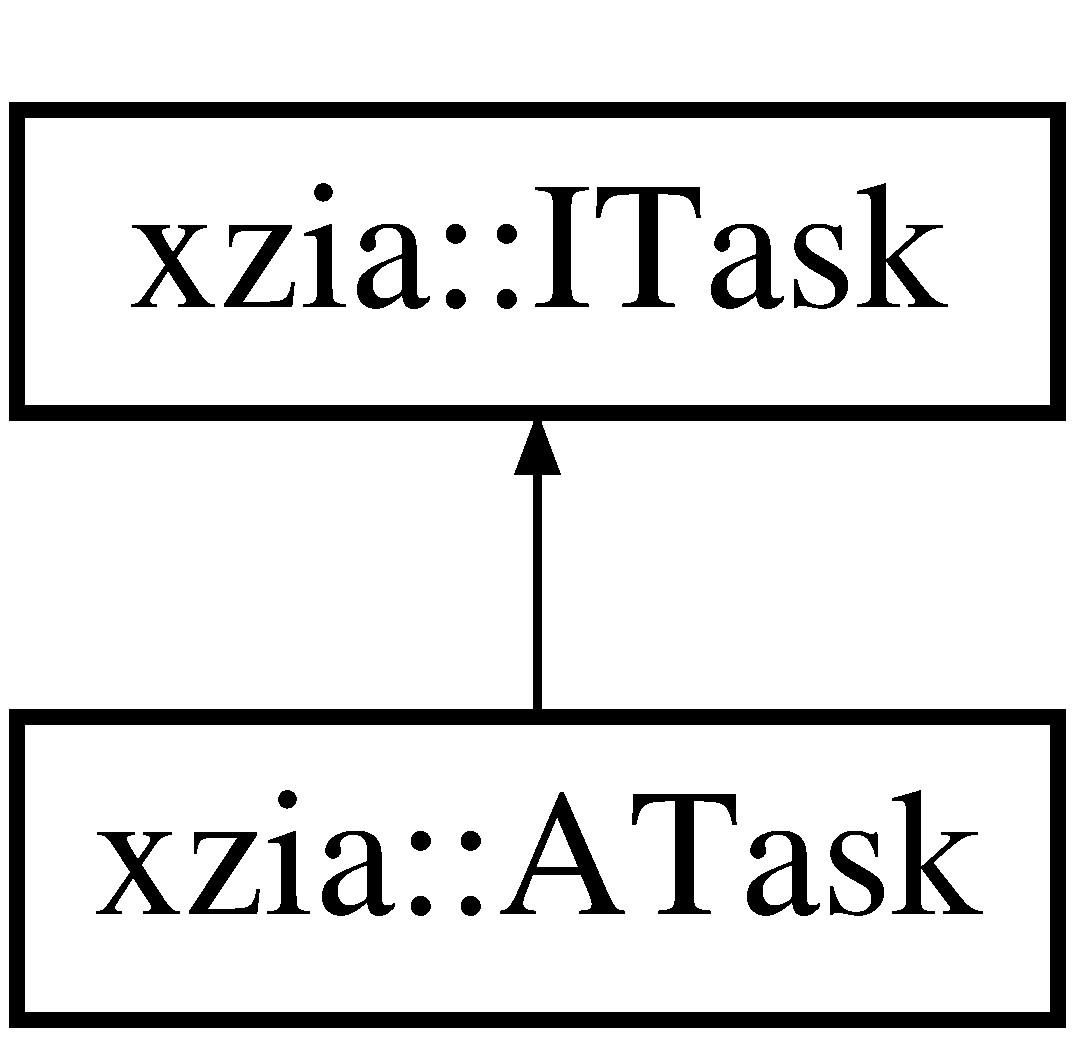
\includegraphics[height=2.000000cm]{classxzia_1_1ITask}
\end{center}
\end{figure}
\subsection*{Public Member Functions}
\begin{DoxyCompactItemize}
\item 
virtual std\+::unique\+\_\+ptr$<$ \mbox{\hyperlink{classxzia_1_1ITask}{I\+Task}} $>$ \mbox{\hyperlink{classxzia_1_1ITask_a7368f69854dd9af5af668e036560226d}{clone}} () const =0
\begin{DoxyCompactList}\small\item\em Clone the current task. \end{DoxyCompactList}\item 
virtual std\+::vector$<$ std\+::unique\+\_\+ptr$<$ \mbox{\hyperlink{classxzia_1_1AHTTPModule}{A\+H\+T\+T\+P\+Module}} $>$ $>$ \& \mbox{\hyperlink{classxzia_1_1ITask_a100285f59380ad90225231734c9a29ab}{get\+Execution\+List}} ()=0
\begin{DoxyCompactList}\small\item\em Get the current list of module. \end{DoxyCompactList}\item 
virtual \mbox{\hyperlink{structxzia_1_1Request}{Request}} const  \& \mbox{\hyperlink{classxzia_1_1ITask_aeac67e104b125e2a9c03ec8a3cd80296}{get\+Request}} () const =0
\begin{DoxyCompactList}\small\item\em Get the current \mbox{\hyperlink{structxzia_1_1Request}{Request}}. \end{DoxyCompactList}\item 
virtual \mbox{\hyperlink{structxzia_1_1Response}{Response}} \& \mbox{\hyperlink{classxzia_1_1ITask_a5bd63caed103f8bf8b6d76a9a802a927}{get\+Response}} ()=0
\begin{DoxyCompactList}\small\item\em Get the current \mbox{\hyperlink{structxzia_1_1Response}{Response}}. \end{DoxyCompactList}\item 
virtual \mbox{\hyperlink{structClient}{Client}} const  \& \mbox{\hyperlink{classxzia_1_1ITask_a2fa35ad0ca8d373c4efd6e928755b5e7}{get\+Client}} () const =0
\begin{DoxyCompactList}\small\item\em Get the current client. \end{DoxyCompactList}\item 
virtual size\+\_\+t \mbox{\hyperlink{classxzia_1_1ITask_a74496410e5dbd3c293082af3d5e7d84f}{get\+Module\+Position}} (\mbox{\hyperlink{classxzia_1_1AHTTPModule}{A\+H\+T\+T\+P\+Module}} const \&module) const =0
\begin{DoxyCompactList}\small\item\em Get a module at a specific position with the module passed in parameter. \end{DoxyCompactList}\item 
virtual \mbox{\hyperlink{classxzia_1_1AHTTPModule}{A\+H\+T\+T\+P\+Module}} \& \mbox{\hyperlink{classxzia_1_1ITask_aa9134b2c523aa55d5f9cfe12866ed508}{get\+Next\+Module}} (std\+::string const \&module\+Name) const =0
\begin{DoxyCompactList}\small\item\em Execution list module getter. \end{DoxyCompactList}\item 
virtual void \mbox{\hyperlink{classxzia_1_1ITask_a0df4e8d2b1391fe1aa7e7bed7d35175e}{push\+Module\+Next}} (std\+::unique\+\_\+ptr$<$ \mbox{\hyperlink{classxzia_1_1AHTTPModule}{A\+H\+T\+T\+P\+Module}} $>$ module)=0
\begin{DoxyCompactList}\small\item\em Push a module in the module list after the current Position. \end{DoxyCompactList}\item 
virtual void \mbox{\hyperlink{classxzia_1_1ITask_a4a742a320f905285dc8fa4510090c381}{push\+Module\+Back}} (std\+::unique\+\_\+ptr$<$ \mbox{\hyperlink{classxzia_1_1AHTTPModule}{A\+H\+T\+T\+P\+Module}} $>$ module)=0
\begin{DoxyCompactList}\small\item\em Push a module at the end of the module list. \end{DoxyCompactList}\item 
virtual void \mbox{\hyperlink{classxzia_1_1ITask_a10e224e38e770108abb3518c06156094}{push\+Module\+At\+Position}} (std\+::unique\+\_\+ptr$<$ \mbox{\hyperlink{classxzia_1_1AHTTPModule}{A\+H\+T\+T\+P\+Module}} $>$ module, size\+\_\+t pos)=0
\begin{DoxyCompactList}\small\item\em Push a module int the module at a specific position. \end{DoxyCompactList}\end{DoxyCompactItemize}


\subsection{Member Function Documentation}
\mbox{\Hypertarget{classxzia_1_1ITask_a7368f69854dd9af5af668e036560226d}\label{classxzia_1_1ITask_a7368f69854dd9af5af668e036560226d}} 
\index{xzia\+::\+I\+Task@{xzia\+::\+I\+Task}!clone@{clone}}
\index{clone@{clone}!xzia\+::\+I\+Task@{xzia\+::\+I\+Task}}
\subsubsection{\texorpdfstring{clone()}{clone()}}
{\footnotesize\ttfamily I\+Task\+::clone (\begin{DoxyParamCaption}{ }\end{DoxyParamCaption}) const\hspace{0.3cm}{\ttfamily [pure virtual]}}



Clone the current task. 

\begin{DoxyReturn}{Returns}
Return a pointer of a clone from the current task. 
\end{DoxyReturn}
\mbox{\Hypertarget{classxzia_1_1ITask_a2fa35ad0ca8d373c4efd6e928755b5e7}\label{classxzia_1_1ITask_a2fa35ad0ca8d373c4efd6e928755b5e7}} 
\index{xzia\+::\+I\+Task@{xzia\+::\+I\+Task}!get\+Client@{get\+Client}}
\index{get\+Client@{get\+Client}!xzia\+::\+I\+Task@{xzia\+::\+I\+Task}}
\subsubsection{\texorpdfstring{get\+Client()}{getClient()}}
{\footnotesize\ttfamily I\+Task\+::get\+Client (\begin{DoxyParamCaption}{ }\end{DoxyParamCaption}) const\hspace{0.3cm}{\ttfamily [pure virtual]}}



Get the current client. 

\begin{DoxyReturn}{Returns}
Return the current \mbox{\hyperlink{structClient}{Client}} id 
\end{DoxyReturn}
\mbox{\Hypertarget{classxzia_1_1ITask_a100285f59380ad90225231734c9a29ab}\label{classxzia_1_1ITask_a100285f59380ad90225231734c9a29ab}} 
\index{xzia\+::\+I\+Task@{xzia\+::\+I\+Task}!get\+Execution\+List@{get\+Execution\+List}}
\index{get\+Execution\+List@{get\+Execution\+List}!xzia\+::\+I\+Task@{xzia\+::\+I\+Task}}
\subsubsection{\texorpdfstring{get\+Execution\+List()}{getExecutionList()}}
{\footnotesize\ttfamily I\+Task\+::get\+Execution\+List (\begin{DoxyParamCaption}{ }\end{DoxyParamCaption})\hspace{0.3cm}{\ttfamily [pure virtual]}}



Get the current list of module. 

\begin{DoxyReturn}{Returns}
Return a vector containing the modules 
\end{DoxyReturn}
\mbox{\Hypertarget{classxzia_1_1ITask_a74496410e5dbd3c293082af3d5e7d84f}\label{classxzia_1_1ITask_a74496410e5dbd3c293082af3d5e7d84f}} 
\index{xzia\+::\+I\+Task@{xzia\+::\+I\+Task}!get\+Module\+Position@{get\+Module\+Position}}
\index{get\+Module\+Position@{get\+Module\+Position}!xzia\+::\+I\+Task@{xzia\+::\+I\+Task}}
\subsubsection{\texorpdfstring{get\+Module\+Position()}{getModulePosition()}}
{\footnotesize\ttfamily I\+Task\+::get\+Module\+Position (\begin{DoxyParamCaption}\item[{\mbox{\hyperlink{classxzia_1_1AHTTPModule}{A\+H\+T\+T\+P\+Module}} const \&}]{module }\end{DoxyParamCaption}) const\hspace{0.3cm}{\ttfamily [pure virtual]}}



Get a module at a specific position with the module passed in parameter. 


\begin{DoxyParams}{Parameters}
{\em module} & Reference of the module we want to get \\
\hline
\end{DoxyParams}
\begin{DoxyReturn}{Returns}
Return the position of the module asked in parameter in the module list 
\end{DoxyReturn}
\mbox{\Hypertarget{classxzia_1_1ITask_aa9134b2c523aa55d5f9cfe12866ed508}\label{classxzia_1_1ITask_aa9134b2c523aa55d5f9cfe12866ed508}} 
\index{xzia\+::\+I\+Task@{xzia\+::\+I\+Task}!get\+Next\+Module@{get\+Next\+Module}}
\index{get\+Next\+Module@{get\+Next\+Module}!xzia\+::\+I\+Task@{xzia\+::\+I\+Task}}
\subsubsection{\texorpdfstring{get\+Next\+Module()}{getNextModule()}}
{\footnotesize\ttfamily I\+Task\+::get\+Next\+Module (\begin{DoxyParamCaption}\item[{std\+::string const \&}]{module\+Name }\end{DoxyParamCaption}) const\hspace{0.3cm}{\ttfamily [pure virtual]}}



Execution list module getter. 


\begin{DoxyParams}{Parameters}
{\em module\+Name} & Module name \\
\hline
\end{DoxyParams}
\begin{DoxyReturn}{Returns}
A reference to the next module searched 
\end{DoxyReturn}
\mbox{\Hypertarget{classxzia_1_1ITask_aeac67e104b125e2a9c03ec8a3cd80296}\label{classxzia_1_1ITask_aeac67e104b125e2a9c03ec8a3cd80296}} 
\index{xzia\+::\+I\+Task@{xzia\+::\+I\+Task}!get\+Request@{get\+Request}}
\index{get\+Request@{get\+Request}!xzia\+::\+I\+Task@{xzia\+::\+I\+Task}}
\subsubsection{\texorpdfstring{get\+Request()}{getRequest()}}
{\footnotesize\ttfamily I\+Task\+::get\+Request (\begin{DoxyParamCaption}{ }\end{DoxyParamCaption}) const\hspace{0.3cm}{\ttfamily [pure virtual]}}



Get the current \mbox{\hyperlink{structxzia_1_1Request}{Request}}. 

\begin{DoxyReturn}{Returns}
Return a reference on the the current \mbox{\hyperlink{structxzia_1_1Request}{Request}} 
\end{DoxyReturn}
\mbox{\Hypertarget{classxzia_1_1ITask_a5bd63caed103f8bf8b6d76a9a802a927}\label{classxzia_1_1ITask_a5bd63caed103f8bf8b6d76a9a802a927}} 
\index{xzia\+::\+I\+Task@{xzia\+::\+I\+Task}!get\+Response@{get\+Response}}
\index{get\+Response@{get\+Response}!xzia\+::\+I\+Task@{xzia\+::\+I\+Task}}
\subsubsection{\texorpdfstring{get\+Response()}{getResponse()}}
{\footnotesize\ttfamily I\+Task\+::get\+Response (\begin{DoxyParamCaption}{ }\end{DoxyParamCaption})\hspace{0.3cm}{\ttfamily [pure virtual]}}



Get the current \mbox{\hyperlink{structxzia_1_1Response}{Response}}. 

\begin{DoxyReturn}{Returns}
Return a reference on the current \mbox{\hyperlink{structxzia_1_1Response}{Response}} 
\end{DoxyReturn}
\mbox{\Hypertarget{classxzia_1_1ITask_a10e224e38e770108abb3518c06156094}\label{classxzia_1_1ITask_a10e224e38e770108abb3518c06156094}} 
\index{xzia\+::\+I\+Task@{xzia\+::\+I\+Task}!push\+Module\+At\+Position@{push\+Module\+At\+Position}}
\index{push\+Module\+At\+Position@{push\+Module\+At\+Position}!xzia\+::\+I\+Task@{xzia\+::\+I\+Task}}
\subsubsection{\texorpdfstring{push\+Module\+At\+Position()}{pushModuleAtPosition()}}
{\footnotesize\ttfamily I\+Task\+::push\+Module\+At\+Position (\begin{DoxyParamCaption}\item[{std\+::unique\+\_\+ptr$<$ \mbox{\hyperlink{classxzia_1_1AHTTPModule}{A\+H\+T\+T\+P\+Module}} $>$}]{module,  }\item[{size\+\_\+t}]{pos }\end{DoxyParamCaption})\hspace{0.3cm}{\ttfamily [pure virtual]}}



Push a module int the module at a specific position. 


\begin{DoxyParams}{Parameters}
{\em module} & Module which going to be set in the module list \\
\hline
{\em pos} & Position where the module is going to be set \\
\hline
\end{DoxyParams}
\mbox{\Hypertarget{classxzia_1_1ITask_a4a742a320f905285dc8fa4510090c381}\label{classxzia_1_1ITask_a4a742a320f905285dc8fa4510090c381}} 
\index{xzia\+::\+I\+Task@{xzia\+::\+I\+Task}!push\+Module\+Back@{push\+Module\+Back}}
\index{push\+Module\+Back@{push\+Module\+Back}!xzia\+::\+I\+Task@{xzia\+::\+I\+Task}}
\subsubsection{\texorpdfstring{push\+Module\+Back()}{pushModuleBack()}}
{\footnotesize\ttfamily I\+Task\+::push\+Module\+Back (\begin{DoxyParamCaption}\item[{std\+::unique\+\_\+ptr$<$ \mbox{\hyperlink{classxzia_1_1AHTTPModule}{A\+H\+T\+T\+P\+Module}} $>$}]{module }\end{DoxyParamCaption})\hspace{0.3cm}{\ttfamily [pure virtual]}}



Push a module at the end of the module list. 


\begin{DoxyParams}{Parameters}
{\em module} & Module which going to be set in the module list \\
\hline
\end{DoxyParams}
\mbox{\Hypertarget{classxzia_1_1ITask_a0df4e8d2b1391fe1aa7e7bed7d35175e}\label{classxzia_1_1ITask_a0df4e8d2b1391fe1aa7e7bed7d35175e}} 
\index{xzia\+::\+I\+Task@{xzia\+::\+I\+Task}!push\+Module\+Next@{push\+Module\+Next}}
\index{push\+Module\+Next@{push\+Module\+Next}!xzia\+::\+I\+Task@{xzia\+::\+I\+Task}}
\subsubsection{\texorpdfstring{push\+Module\+Next()}{pushModuleNext()}}
{\footnotesize\ttfamily I\+Task\+::push\+Module\+Next (\begin{DoxyParamCaption}\item[{std\+::unique\+\_\+ptr$<$ \mbox{\hyperlink{classxzia_1_1AHTTPModule}{A\+H\+T\+T\+P\+Module}} $>$}]{module }\end{DoxyParamCaption})\hspace{0.3cm}{\ttfamily [pure virtual]}}



Push a module in the module list after the current Position. 


\begin{DoxyParams}{Parameters}
{\em module} & Module which going to be set in the module list \\
\hline
\end{DoxyParams}


The documentation for this class was generated from the following file\+:\begin{DoxyCompactItemize}
\item 
/home/edouard/\+Documents/2017/\+Z\+I\+A/\+Existen\+Z\+I\+A/\+A\+P\+I/include/task/\mbox{\hyperlink{ITask_8hpp}{I\+Task.\+hpp}}\end{DoxyCompactItemize}

\hypertarget{classITaskFactory}{}\section{I\+Task\+Factory Class Reference}
\label{classITaskFactory}\index{I\+Task\+Factory@{I\+Task\+Factory}}


The documentation for this class was generated from the following file\+:\begin{DoxyCompactItemize}
\item 
/home/edouard/\+Documents/2017/\+Z\+I\+A/\+Existen\+Z\+I\+A/\+A\+P\+I/include/task/\mbox{\hyperlink{ITaskFactory_8hpp}{I\+Task\+Factory.\+hpp}}\end{DoxyCompactItemize}

\hypertarget{classxzia_1_1ITaskFactory}{}\section{xzia\+:\+:I\+Task\+Factory Class Reference}
\label{classxzia_1_1ITaskFactory}\index{xzia\+::\+I\+Task\+Factory@{xzia\+::\+I\+Task\+Factory}}
Inheritance diagram for xzia\+:\+:I\+Task\+Factory\+:\begin{figure}[H]
\begin{center}
\leavevmode
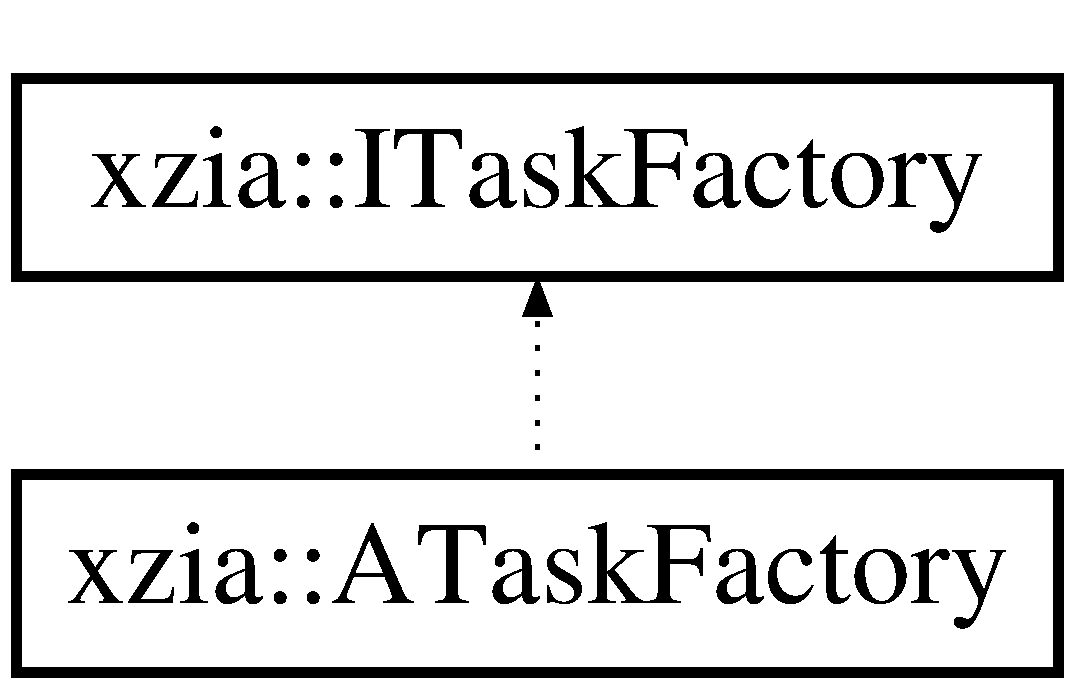
\includegraphics[height=2.000000cm]{classxzia_1_1ITaskFactory}
\end{center}
\end{figure}
\subsection*{Public Member Functions}
\begin{DoxyCompactItemize}
\item 
\mbox{\Hypertarget{classxzia_1_1ITaskFactory_a2fdce8ea701c55eb73d00efd8f367c2c}\label{classxzia_1_1ITaskFactory_a2fdce8ea701c55eb73d00efd8f367c2c}} 
virtual std\+::unique\+\_\+ptr$<$ \mbox{\hyperlink{classxzia_1_1ATask}{A\+Task}} $>$ {\bfseries create\+Task} (std\+::unique\+\_\+ptr$<$ \mbox{\hyperlink{structxzia_1_1Request}{Request}} $>$ req, \mbox{\hyperlink{structClient}{Client}} client)=0
\end{DoxyCompactItemize}


The documentation for this class was generated from the following file\+:\begin{DoxyCompactItemize}
\item 
/home/edouard/\+Documents/2017/\+Z\+I\+A/\+Existen\+Z\+I\+A/\+A\+P\+I/include/task/I\+Task\+Factory.\+hpp\end{DoxyCompactItemize}

\hypertarget{classIThreadPool}{}\section{I\+Thread\+Pool Class Reference}
\label{classIThreadPool}\index{I\+Thread\+Pool@{I\+Thread\+Pool}}


The documentation for this class was generated from the following file\+:\begin{DoxyCompactItemize}
\item 
/home/edouard/\+Documents/2017/\+Z\+I\+A/\+Existen\+Z\+I\+A/\+A\+P\+I/include/thread/\mbox{\hyperlink{IThreadPool_8hpp}{I\+Thread\+Pool.\+hpp}}\end{DoxyCompactItemize}

\hypertarget{classxzia_1_1IThreadPool}{}\section{xzia\+:\+:I\+Thread\+Pool Class Reference}
\label{classxzia_1_1IThreadPool}\index{xzia\+::\+I\+Thread\+Pool@{xzia\+::\+I\+Thread\+Pool}}
Inheritance diagram for xzia\+:\+:I\+Thread\+Pool\+:\begin{figure}[H]
\begin{center}
\leavevmode
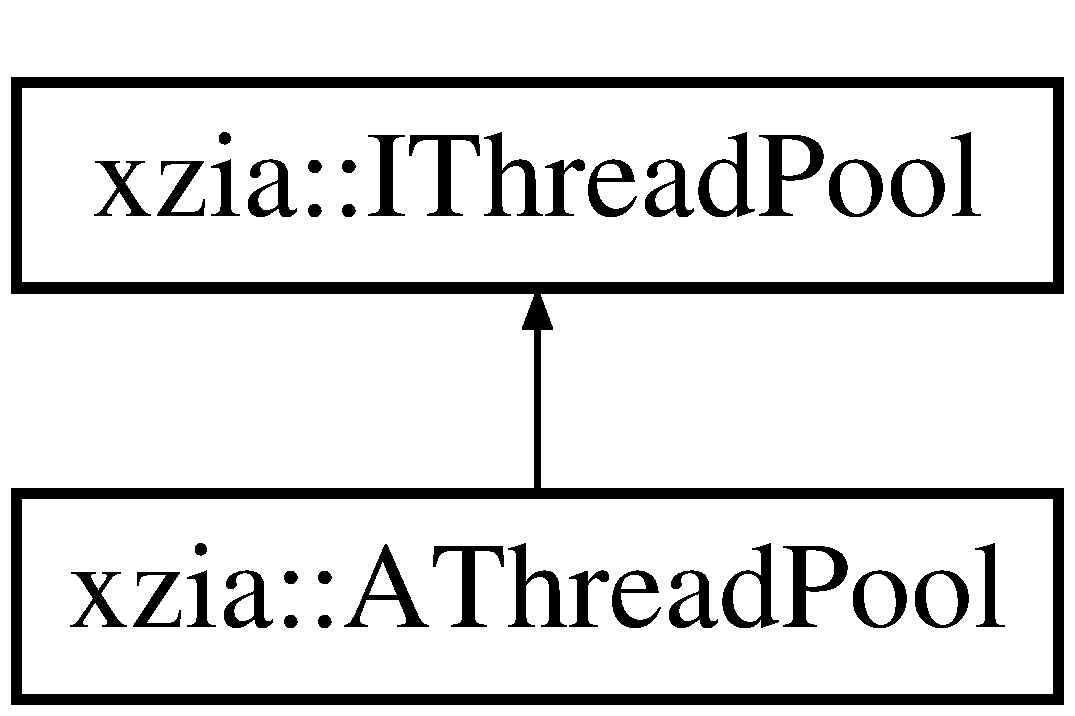
\includegraphics[height=2.000000cm]{classxzia_1_1IThreadPool}
\end{center}
\end{figure}
\subsection*{Public Member Functions}
\begin{DoxyCompactItemize}
\item 
virtual void \mbox{\hyperlink{classxzia_1_1IThreadPool_adf16985d0215c0cfafe57f3c056d2983}{add\+Task}} (std\+::unique\+\_\+ptr$<$ \mbox{\hyperlink{classxzia_1_1ATask}{A\+Task}} $>$ task)=0
\begin{DoxyCompactList}\small\item\em Add a task to the work\+Flow thread. \end{DoxyCompactList}\item 
\mbox{\Hypertarget{classxzia_1_1IThreadPool_add8ae9a80915f75f55ebdb25786cedf4}\label{classxzia_1_1IThreadPool_add8ae9a80915f75f55ebdb25786cedf4}} 
virtual void \mbox{\hyperlink{classxzia_1_1IThreadPool_add8ae9a80915f75f55ebdb25786cedf4}{stop}} ()=0
\begin{DoxyCompactList}\small\item\em Stop the thread. \end{DoxyCompactList}\item 
\mbox{\Hypertarget{classxzia_1_1IThreadPool_af48f08840decdd834631d9ec5648cf36}\label{classxzia_1_1IThreadPool_af48f08840decdd834631d9ec5648cf36}} 
virtual std\+::vector$<$ std\+::unique\+\_\+ptr$<$ \mbox{\hyperlink{classxzia_1_1ATask}{A\+Task}} $>$ $>$ {\bfseries get\+All\+Task\+Done} ()=0
\end{DoxyCompactItemize}


\subsection{Member Function Documentation}
\mbox{\Hypertarget{classxzia_1_1IThreadPool_adf16985d0215c0cfafe57f3c056d2983}\label{classxzia_1_1IThreadPool_adf16985d0215c0cfafe57f3c056d2983}} 
\index{xzia\+::\+I\+Thread\+Pool@{xzia\+::\+I\+Thread\+Pool}!add\+Task@{add\+Task}}
\index{add\+Task@{add\+Task}!xzia\+::\+I\+Thread\+Pool@{xzia\+::\+I\+Thread\+Pool}}
\subsubsection{\texorpdfstring{add\+Task()}{addTask()}}
{\footnotesize\ttfamily I\+Thread\+Pool\+::add\+Task (\begin{DoxyParamCaption}\item[{std\+::unique\+\_\+ptr$<$ \mbox{\hyperlink{classxzia_1_1ATask}{A\+Task}} $>$}]{task }\end{DoxyParamCaption})\hspace{0.3cm}{\ttfamily [pure virtual]}}



Add a task to the work\+Flow thread. 


\begin{DoxyParams}{Parameters}
{\em task} & Task to process \\
\hline
\end{DoxyParams}


The documentation for this class was generated from the following file\+:\begin{DoxyCompactItemize}
\item 
/home/edouard/\+Documents/2017/\+Z\+I\+A/\+Existen\+Z\+I\+A/\+A\+P\+I/include/thread/\mbox{\hyperlink{IThreadPool_8hpp}{I\+Thread\+Pool.\+hpp}}\end{DoxyCompactItemize}

\hypertarget{structMessage}{}\section{Message Struct Reference}
\label{structMessage}\index{Message@{Message}}


The documentation for this struct was generated from the following file\+:\begin{DoxyCompactItemize}
\item 
/home/edouard/\+Documents/2017/\+Z\+I\+A/\+Existen\+Z\+I\+A/\+A\+P\+I/include/http/\mbox{\hyperlink{Message_8hpp}{Message.\+hpp}}\end{DoxyCompactItemize}

\hypertarget{structxzia_1_1Message}{}\section{xzia\+:\+:Message Struct Reference}
\label{structxzia_1_1Message}\index{xzia\+::\+Message@{xzia\+::\+Message}}
Inheritance diagram for xzia\+:\+:Message\+:\begin{figure}[H]
\begin{center}
\leavevmode
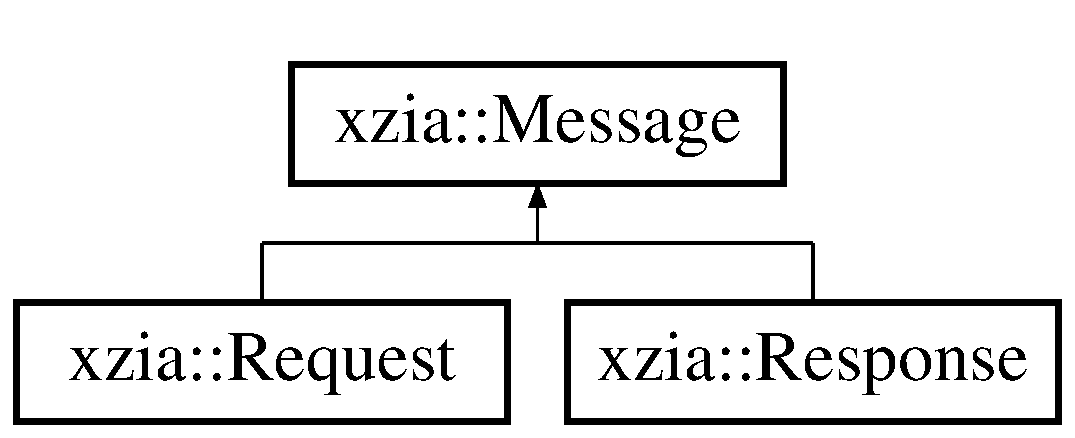
\includegraphics[height=2.000000cm]{structxzia_1_1Message}
\end{center}
\end{figure}
\subsection*{Public Member Functions}
\begin{DoxyCompactItemize}
\item 
\mbox{\Hypertarget{structxzia_1_1Message_a8f266edc36c0d6dca420e67547a91547}\label{structxzia_1_1Message_a8f266edc36c0d6dca420e67547a91547}} 
{\bfseries Message} (\mbox{\hyperlink{structClient}{Client}} client)
\item 
bool \mbox{\hyperlink{structxzia_1_1Message_a096560e32a7b9dd61421770fc0199402}{has\+Body}} ()
\end{DoxyCompactItemize}
\subsection*{Public Attributes}
\begin{DoxyCompactItemize}
\item 
\mbox{\Hypertarget{structxzia_1_1Message_a39985c243bca49b58e9295655473acf8}\label{structxzia_1_1Message_a39985c243bca49b58e9295655473acf8}} 
std\+::string {\bfseries body}
\item 
\mbox{\Hypertarget{structxzia_1_1Message_af7dbb8337a84b35014d2389b8ca41073}\label{structxzia_1_1Message_af7dbb8337a84b35014d2389b8ca41073}} 
std\+::string {\bfseries version}
\item 
\mbox{\Hypertarget{structxzia_1_1Message_a8c20098d713f5546ffb8486d730045d2}\label{structxzia_1_1Message_a8c20098d713f5546ffb8486d730045d2}} 
std\+::map$<$ std\+::string, std\+::string $>$ {\bfseries header}
\item 
\mbox{\Hypertarget{structxzia_1_1Message_a6af0c43aad93c5f4e7f252c813c9fb27}\label{structxzia_1_1Message_a6af0c43aad93c5f4e7f252c813c9fb27}} 
\mbox{\hyperlink{structClient}{Client}} const {\bfseries client}
\end{DoxyCompactItemize}


\subsection{Member Function Documentation}
\mbox{\Hypertarget{structxzia_1_1Message_a096560e32a7b9dd61421770fc0199402}\label{structxzia_1_1Message_a096560e32a7b9dd61421770fc0199402}} 
\index{xzia\+::\+Message@{xzia\+::\+Message}!has\+Body@{has\+Body}}
\index{has\+Body@{has\+Body}!xzia\+::\+Message@{xzia\+::\+Message}}
\subsubsection{\texorpdfstring{has\+Body()}{hasBody()}}
{\footnotesize\ttfamily Message\+::has\+Body (\begin{DoxyParamCaption}{ }\end{DoxyParamCaption})}

\begin{DoxyReturn}{Returns}
Return True if the message has a body, else false 
\end{DoxyReturn}


The documentation for this struct was generated from the following files\+:\begin{DoxyCompactItemize}
\item 
/home/edouard/\+Documents/2017/\+Z\+I\+A/\+Existen\+Z\+I\+A/\+A\+P\+I/include/http/\mbox{\hyperlink{Message_8hpp}{Message.\+hpp}}\item 
/home/edouard/\+Documents/2017/\+Z\+I\+A/\+Existen\+Z\+I\+A/\+A\+P\+I/src/http/Message.\+cpp\end{DoxyCompactItemize}

\hypertarget{structxzia_1_1Request}{}\section{xzia\+:\+:Request Struct Reference}
\label{structxzia_1_1Request}\index{xzia\+::\+Request@{xzia\+::\+Request}}
Inheritance diagram for xzia\+:\+:Request\+:\begin{figure}[H]
\begin{center}
\leavevmode
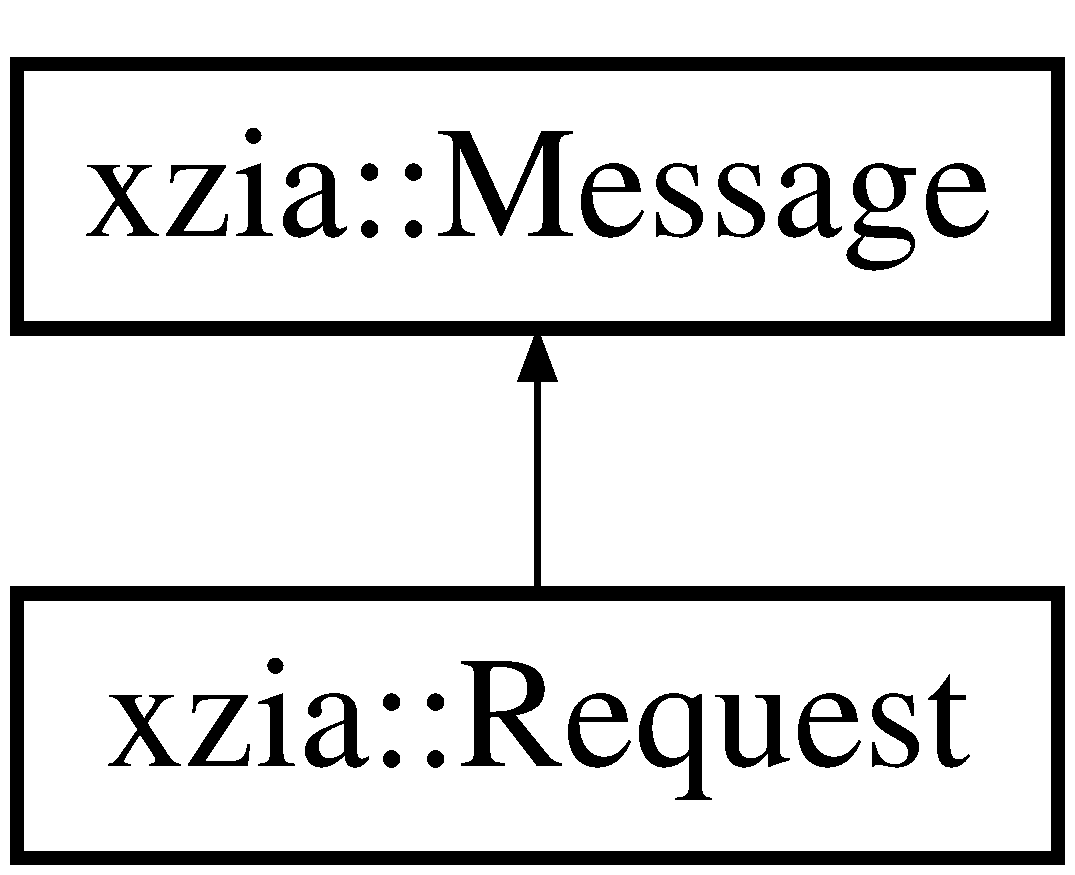
\includegraphics[height=2.000000cm]{structxzia_1_1Request}
\end{center}
\end{figure}
\subsection*{Public Attributes}
\begin{DoxyCompactItemize}
\item 
\mbox{\Hypertarget{structxzia_1_1Request_a74e36e609c8c5006d9afb047470ae6d2}\label{structxzia_1_1Request_a74e36e609c8c5006d9afb047470ae6d2}} 
std\+::string {\bfseries method}
\item 
\mbox{\Hypertarget{structxzia_1_1Request_afd11f14da69728f1957678d625cbfc35}\label{structxzia_1_1Request_afd11f14da69728f1957678d625cbfc35}} 
std\+::string {\bfseries version}
\item 
\mbox{\Hypertarget{structxzia_1_1Request_abfa79948642c0dedd46ffd0f2794d884}\label{structxzia_1_1Request_abfa79948642c0dedd46ffd0f2794d884}} 
std\+::string {\bfseries host}
\item 
\mbox{\Hypertarget{structxzia_1_1Request_a83970c10f1b468d8fc21214187f38fee}\label{structxzia_1_1Request_a83970c10f1b468d8fc21214187f38fee}} 
std\+::string {\bfseries port}
\item 
\mbox{\Hypertarget{structxzia_1_1Request_a2994936d8e244e609837ffcf9515d3b4}\label{structxzia_1_1Request_a2994936d8e244e609837ffcf9515d3b4}} 
std\+::string {\bfseries path}
\item 
\mbox{\Hypertarget{structxzia_1_1Request_a66dacb2e30a35d80485d8366e4bc262b}\label{structxzia_1_1Request_a66dacb2e30a35d80485d8366e4bc262b}} 
std\+::map$<$ std\+::string, std\+::string $>$ {\bfseries query}
\end{DoxyCompactItemize}
\subsection*{Additional Inherited Members}


The documentation for this struct was generated from the following file\+:\begin{DoxyCompactItemize}
\item 
/home/edouard/\+Documents/2017/\+Z\+I\+A/\+Existen\+Z\+I\+A/\+A\+P\+I/include/http/\mbox{\hyperlink{Request_8hpp}{Request.\+hpp}}\end{DoxyCompactItemize}

\hypertarget{structRequest}{}\section{Request Struct Reference}
\label{structRequest}\index{Request@{Request}}


The documentation for this struct was generated from the following file\+:\begin{DoxyCompactItemize}
\item 
/home/edouard/\+Documents/2017/\+Z\+I\+A/\+Existen\+Z\+I\+A/\+A\+P\+I/include/http/\mbox{\hyperlink{Request_8hpp}{Request.\+hpp}}\end{DoxyCompactItemize}

\hypertarget{structxzia_1_1Response}{}\section{xzia\+:\+:Response Struct Reference}
\label{structxzia_1_1Response}\index{xzia\+::\+Response@{xzia\+::\+Response}}
Inheritance diagram for xzia\+:\+:Response\+:\begin{figure}[H]
\begin{center}
\leavevmode
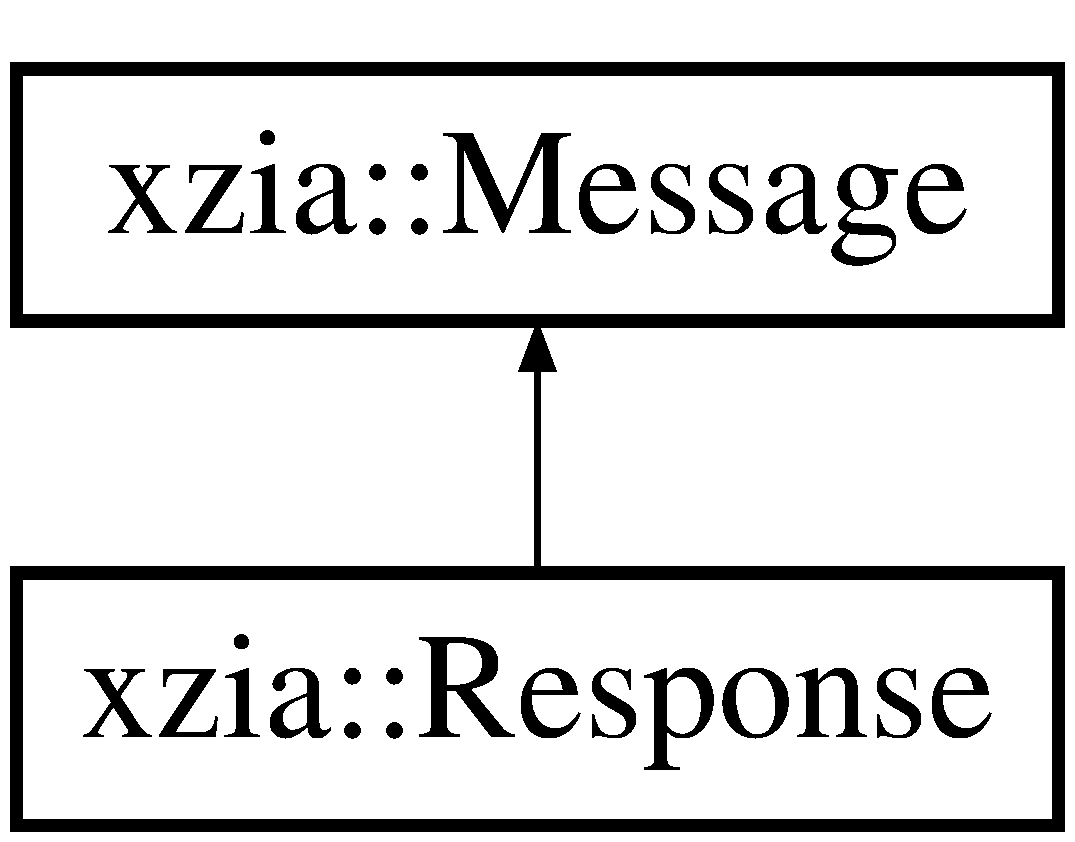
\includegraphics[height=2.000000cm]{structxzia_1_1Response}
\end{center}
\end{figure}
\subsection*{Public Member Functions}
\begin{DoxyCompactItemize}
\item 
\mbox{\Hypertarget{structxzia_1_1Response_a05b2024d7e53aaf5c74f0a0f67f85afd}\label{structxzia_1_1Response_a05b2024d7e53aaf5c74f0a0f67f85afd}} 
{\bfseries Response} (\mbox{\hyperlink{structClient}{Client}} client)
\end{DoxyCompactItemize}
\subsection*{Public Attributes}
\begin{DoxyCompactItemize}
\item 
\mbox{\Hypertarget{structxzia_1_1Response_a694b2aca5178bc4569aeffb7e38ef246}\label{structxzia_1_1Response_a694b2aca5178bc4569aeffb7e38ef246}} 
int {\bfseries code}
\end{DoxyCompactItemize}


The documentation for this struct was generated from the following files\+:\begin{DoxyCompactItemize}
\item 
/home/edouard/\+Documents/2017/\+Z\+I\+A/\+Existen\+Z\+I\+A/\+A\+P\+I/include/http/\mbox{\hyperlink{Response_8hpp}{Response.\+hpp}}\item 
/home/edouard/\+Documents/2017/\+Z\+I\+A/\+Existen\+Z\+I\+A/\+A\+P\+I/src/http/Response.\+cpp\end{DoxyCompactItemize}

\hypertarget{structResponse}{}\section{Response Struct Reference}
\label{structResponse}\index{Response@{Response}}


The documentation for this struct was generated from the following file\+:\begin{DoxyCompactItemize}
\item 
/home/edouard/\+Documents/2017/\+Z\+I\+A/\+Existen\+Z\+I\+A/\+A\+P\+I/include/http/\mbox{\hyperlink{Response_8hpp}{Response.\+hpp}}\end{DoxyCompactItemize}

\chapter{File Documentation}
\hypertarget{Client_8hpp}{}\section{/home/edouard/\+Documents/2017/\+Z\+I\+A/\+Existen\+Z\+I\+A/\+A\+P\+I/include/client/\+Client.hpp File Reference}
\label{Client_8hpp}\index{/home/edouard/\+Documents/2017/\+Z\+I\+A/\+Existen\+Z\+I\+A/\+A\+P\+I/include/client/\+Client.\+hpp@{/home/edouard/\+Documents/2017/\+Z\+I\+A/\+Existen\+Z\+I\+A/\+A\+P\+I/include/client/\+Client.\+hpp}}


Typedef the socket \mbox{\hyperlink{structClient}{Client}} as an int.  


\subsection*{Typedefs}
\begin{DoxyCompactItemize}
\item 
\mbox{\Hypertarget{Client_8hpp_a0b6d1e709e685f96609e9174d43f398f}\label{Client_8hpp_a0b6d1e709e685f96609e9174d43f398f}} 
using {\bfseries xzia\+::\+Client} = int
\end{DoxyCompactItemize}


\subsection{Detailed Description}
Typedef the socket \mbox{\hyperlink{structClient}{Client}} as an int. 

\begin{DoxyAuthor}{Author}
Edouard.\+P 
\end{DoxyAuthor}
\begin{DoxyVersion}{Version}
0.\+1 
\end{DoxyVersion}
\begin{DoxyDate}{Date}
17 novembre 2017 
\end{DoxyDate}

\hypertarget{ACore_8hpp}{}\section{/home/edouard/\+Documents/2017/\+Z\+I\+A/\+Existen\+Z\+I\+A/\+A\+P\+I/include/core/\+A\+Core.hpp File Reference}
\label{ACore_8hpp}\index{/home/edouard/\+Documents/2017/\+Z\+I\+A/\+Existen\+Z\+I\+A/\+A\+P\+I/include/core/\+A\+Core.\+hpp@{/home/edouard/\+Documents/2017/\+Z\+I\+A/\+Existen\+Z\+I\+A/\+A\+P\+I/include/core/\+A\+Core.\+hpp}}


Kernel of the A\+PI, \mbox{\hyperlink{structACore}{A\+Core}} is the class linked to all other classes.  


{\ttfamily \#include $<$vector$>$}\newline
{\ttfamily \#include \char`\"{}task/\+A\+Task\+Factory.\+hpp\char`\"{}}\newline
{\ttfamily \#include \char`\"{}task/\+I\+Task\+Factory.\+hpp\char`\"{}}\newline
{\ttfamily \#include \char`\"{}thread/\+A\+Thread\+Pool.\+hpp\char`\"{}}\newline
{\ttfamily \#include \char`\"{}network/\+I\+Network.\+hpp\char`\"{}}\newline
{\ttfamily \#include \char`\"{}modules/\+A\+Module\+Manager.\+hpp\char`\"{}}\newline
{\ttfamily \#include \char`\"{}loader/\+I\+Loader.\+hpp\char`\"{}}\newline
{\ttfamily \#include \char`\"{}client/\+Client.\+hpp\char`\"{}}\newline
{\ttfamily \#include \char`\"{}I\+Core.\+hpp\char`\"{}}\newline
\subsection*{Classes}
\begin{DoxyCompactItemize}
\item 
class \mbox{\hyperlink{classxzia_1_1ACore}{xzia\+::\+A\+Core}}
\end{DoxyCompactItemize}


\subsection{Detailed Description}
Kernel of the A\+PI, \mbox{\hyperlink{structACore}{A\+Core}} is the class linked to all other classes. 

\begin{DoxyAuthor}{Author}
Edouard.\+P 
\end{DoxyAuthor}
\begin{DoxyVersion}{Version}
0.\+1 
\end{DoxyVersion}
\begin{DoxyDate}{Date}
17 novembre 2017 
\end{DoxyDate}

\hypertarget{ICore_8hpp}{}\section{/home/edouard/\+Documents/2017/\+Z\+I\+A/\+Existen\+Z\+I\+A/\+A\+P\+I/include/core/\+I\+Core.hpp File Reference}
\label{ICore_8hpp}\index{/home/edouard/\+Documents/2017/\+Z\+I\+A/\+Existen\+Z\+I\+A/\+A\+P\+I/include/core/\+I\+Core.\+hpp@{/home/edouard/\+Documents/2017/\+Z\+I\+A/\+Existen\+Z\+I\+A/\+A\+P\+I/include/core/\+I\+Core.\+hpp}}


Interface of the main class of the A\+PI.  


\subsection*{Classes}
\begin{DoxyCompactItemize}
\item 
class \mbox{\hyperlink{classxzia_1_1ICore}{xzia\+::\+I\+Core}}
\end{DoxyCompactItemize}


\subsection{Detailed Description}
Interface of the main class of the A\+PI. 

\begin{DoxyAuthor}{Author}
Pierre.\+B 
\end{DoxyAuthor}
\begin{DoxyVersion}{Version}
0.\+1 
\end{DoxyVersion}
\begin{DoxyDate}{Date}
17 novembre 2017 
\end{DoxyDate}

\hypertarget{Message_8hpp}{}\section{/home/edouard/\+Documents/2017/\+Z\+I\+A/\+Existen\+Z\+I\+A/\+A\+P\+I/include/http/\+Message.hpp File Reference}
\label{Message_8hpp}\index{/home/edouard/\+Documents/2017/\+Z\+I\+A/\+Existen\+Z\+I\+A/\+A\+P\+I/include/http/\+Message.\+hpp@{/home/edouard/\+Documents/2017/\+Z\+I\+A/\+Existen\+Z\+I\+A/\+A\+P\+I/include/http/\+Message.\+hpp}}


\mbox{\hyperlink{structMessage}{Message}} is a structure which contain all the information about the request. It can be either a request to ask information or a response for the return of a request.  


{\ttfamily \#include $<$iostream$>$}\newline
{\ttfamily \#include $<$map$>$}\newline
{\ttfamily \#include $<$client/\+Client.\+hpp$>$}\newline
\subsection*{Classes}
\begin{DoxyCompactItemize}
\item 
struct \mbox{\hyperlink{structxzia_1_1Message}{xzia\+::\+Message}}
\end{DoxyCompactItemize}


\subsection{Detailed Description}
\mbox{\hyperlink{structMessage}{Message}} is a structure which contain all the information about the request. It can be either a request to ask information or a response for the return of a request. 

\begin{DoxyAuthor}{Author}
Robin.\+U 
\end{DoxyAuthor}
\begin{DoxyVersion}{Version}
0.\+1 
\end{DoxyVersion}
\begin{DoxyDate}{Date}
13 novembre 2017 
\end{DoxyDate}

\hypertarget{Request_8hpp}{}\section{/home/edouard/\+Documents/2017/\+Z\+I\+A/\+Existen\+Z\+I\+A/\+A\+P\+I/include/http/\+Request.hpp File Reference}
\label{Request_8hpp}\index{/home/edouard/\+Documents/2017/\+Z\+I\+A/\+Existen\+Z\+I\+A/\+A\+P\+I/include/http/\+Request.\+hpp@{/home/edouard/\+Documents/2017/\+Z\+I\+A/\+Existen\+Z\+I\+A/\+A\+P\+I/include/http/\+Request.\+hpp}}


\mbox{\hyperlink{structRequest}{Request}} is a specific message which goal is to ask something and wait for a response.  


{\ttfamily \#include $<$iostream$>$}\newline
{\ttfamily \#include \char`\"{}Message.\+hpp\char`\"{}}\newline
\subsection*{Classes}
\begin{DoxyCompactItemize}
\item 
struct \mbox{\hyperlink{structxzia_1_1Request}{xzia\+::\+Request}}
\end{DoxyCompactItemize}


\subsection{Detailed Description}
\mbox{\hyperlink{structRequest}{Request}} is a specific message which goal is to ask something and wait for a response. 

\begin{DoxyAuthor}{Author}
Benjamin.\+D 
\end{DoxyAuthor}
\begin{DoxyVersion}{Version}
0.\+1 
\end{DoxyVersion}
\begin{DoxyDate}{Date}
17 novembre 2017 
\end{DoxyDate}

\hypertarget{Response_8hpp}{}\section{/home/edouard/\+Documents/2017/\+Z\+I\+A/\+Existen\+Z\+I\+A/\+A\+P\+I/include/http/\+Response.hpp File Reference}
\label{Response_8hpp}\index{/home/edouard/\+Documents/2017/\+Z\+I\+A/\+Existen\+Z\+I\+A/\+A\+P\+I/include/http/\+Response.\+hpp@{/home/edouard/\+Documents/2017/\+Z\+I\+A/\+Existen\+Z\+I\+A/\+A\+P\+I/include/http/\+Response.\+hpp}}


\mbox{\hyperlink{structResponse}{Response}} is a specific message which goal is to return a message containing the result code of the task asked.  


{\ttfamily \#include \char`\"{}Message.\+hpp\char`\"{}}\newline
\subsection*{Classes}
\begin{DoxyCompactItemize}
\item 
struct \mbox{\hyperlink{structxzia_1_1Response}{xzia\+::\+Response}}
\end{DoxyCompactItemize}


\subsection{Detailed Description}
\mbox{\hyperlink{structResponse}{Response}} is a specific message which goal is to return a message containing the result code of the task asked. 

\begin{DoxyAuthor}{Author}
Pierre.\+B 
\end{DoxyAuthor}
\begin{DoxyVersion}{Version}
0.\+1 
\end{DoxyVersion}
\begin{DoxyDate}{Date}
13 novembre 2017 
\end{DoxyDate}

\hypertarget{ALoader_8hpp}{}\section{/home/edouard/\+Documents/2017/\+Z\+I\+A/\+Existen\+Z\+I\+A/\+A\+P\+I/include/loader/\+A\+Loader.hpp File Reference}
\label{ALoader_8hpp}\index{/home/edouard/\+Documents/2017/\+Z\+I\+A/\+Existen\+Z\+I\+A/\+A\+P\+I/include/loader/\+A\+Loader.\+hpp@{/home/edouard/\+Documents/2017/\+Z\+I\+A/\+Existen\+Z\+I\+A/\+A\+P\+I/include/loader/\+A\+Loader.\+hpp}}


\mbox{\hyperlink{classALoader}{A\+Loader}} manages the dynamic loading of the modules and the configuration of those according to the configuration loader.  


{\ttfamily \#include $<$memory$>$}\newline
{\ttfamily \#include \char`\"{}I\+Loader.\+hpp\char`\"{}}\newline
{\ttfamily \#include \char`\"{}I\+Config\+Loader.\+hpp\char`\"{}}\newline
\subsection*{Classes}
\begin{DoxyCompactItemize}
\item 
class \mbox{\hyperlink{classxzia_1_1ALoader}{xzia\+::\+A\+Loader}}
\end{DoxyCompactItemize}


\subsection{Detailed Description}
\mbox{\hyperlink{classALoader}{A\+Loader}} manages the dynamic loading of the modules and the configuration of those according to the configuration loader. 

\begin{DoxyAuthor}{Author}
Edouard.\+P 
\end{DoxyAuthor}
\begin{DoxyVersion}{Version}
0.\+1 
\end{DoxyVersion}
\begin{DoxyDate}{Date}
16 novembre 2017 
\end{DoxyDate}

\hypertarget{IConfigLoader_8hpp}{}\section{/home/edouard/\+Documents/2017/\+Z\+I\+A/\+Existen\+Z\+I\+A/\+A\+P\+I/include/loader/\+I\+Config\+Loader.hpp File Reference}
\label{IConfigLoader_8hpp}\index{/home/edouard/\+Documents/2017/\+Z\+I\+A/\+Existen\+Z\+I\+A/\+A\+P\+I/include/loader/\+I\+Config\+Loader.\+hpp@{/home/edouard/\+Documents/2017/\+Z\+I\+A/\+Existen\+Z\+I\+A/\+A\+P\+I/include/loader/\+I\+Config\+Loader.\+hpp}}
{\ttfamily \#include $<$iostream$>$}\newline
{\ttfamily \#include $<$map$>$}\newline
{\ttfamily \#include $<$vector$>$}\newline
\subsection*{Classes}
\begin{DoxyCompactItemize}
\item 
class \mbox{\hyperlink{classxzia_1_1IConfigLoader}{xzia\+::\+I\+Config\+Loader}}
\end{DoxyCompactItemize}


\subsection{Detailed Description}
\begin{DoxyAuthor}{Author}
Pierre.\+B 
\end{DoxyAuthor}
\begin{DoxyVersion}{Version}
0.\+1 
\end{DoxyVersion}
\begin{DoxyDate}{Date}
17 novembre 2017
\end{DoxyDate}
This interface ensure that we can ask the configuration of a specific module or the core. This configuration shall appear in the form of a simple map of strings \mbox{[}K\+EY,V\+A\+L\+UE\mbox{]} 
\hypertarget{ILoader_8hpp}{}\section{/home/edouard/\+Documents/2017/\+Z\+I\+A/\+Existen\+Z\+I\+A/\+A\+P\+I/include/loader/\+I\+Loader.hpp File Reference}
\label{ILoader_8hpp}\index{/home/edouard/\+Documents/2017/\+Z\+I\+A/\+Existen\+Z\+I\+A/\+A\+P\+I/include/loader/\+I\+Loader.\+hpp@{/home/edouard/\+Documents/2017/\+Z\+I\+A/\+Existen\+Z\+I\+A/\+A\+P\+I/include/loader/\+I\+Loader.\+hpp}}


Used to load modules and their configurations.  


{\ttfamily \#include $<$iostream$>$}\newline
{\ttfamily \#include $<$map$>$}\newline
{\ttfamily \#include $<$vector$>$}\newline
{\ttfamily \#include \char`\"{}modules/\+A\+Module.\+hpp\char`\"{}}\newline
\subsection*{Classes}
\begin{DoxyCompactItemize}
\item 
class \mbox{\hyperlink{classxzia_1_1ILoader}{xzia\+::\+I\+Loader}}
\end{DoxyCompactItemize}


\subsection{Detailed Description}
Used to load modules and their configurations. 

\begin{DoxyAuthor}{Author}
Edouard.\+P 
\end{DoxyAuthor}
\begin{DoxyVersion}{Version}
0.\+1 
\end{DoxyVersion}
\begin{DoxyDate}{Date}
13 novembre 2017
\end{DoxyDate}
add comment here 
\hypertarget{AHTTPModule_8hpp}{}\section{/home/edouard/\+Documents/2017/\+Z\+I\+A/\+Existen\+Z\+I\+A/\+A\+P\+I/include/modules/\+A\+H\+T\+T\+P\+Module.hpp File Reference}
\label{AHTTPModule_8hpp}\index{/home/edouard/\+Documents/2017/\+Z\+I\+A/\+Existen\+Z\+I\+A/\+A\+P\+I/include/modules/\+A\+H\+T\+T\+P\+Module.\+hpp@{/home/edouard/\+Documents/2017/\+Z\+I\+A/\+Existen\+Z\+I\+A/\+A\+P\+I/include/modules/\+A\+H\+T\+T\+P\+Module.\+hpp}}


Standard module that is used in the task execution list.  


{\ttfamily \#include \char`\"{}A\+Module.\+hpp\char`\"{}}\newline
{\ttfamily \#include \char`\"{}Data\+Store.\+hpp\char`\"{}}\newline
{\ttfamily \#include \char`\"{}Step.\+hpp\char`\"{}}\newline
\subsection*{Classes}
\begin{DoxyCompactItemize}
\item 
class \mbox{\hyperlink{classxzia_1_1AHTTPModule}{xzia\+::\+A\+H\+T\+T\+P\+Module}}
\end{DoxyCompactItemize}


\subsection{Detailed Description}
Standard module that is used in the task execution list. 

\begin{DoxyAuthor}{Author}
Matthieu.\+S 
\end{DoxyAuthor}
\begin{DoxyVersion}{Version}
0.\+1 
\end{DoxyVersion}
\begin{DoxyDate}{Date}
16 novembre 2017 
\end{DoxyDate}

\hypertarget{AModule_8hpp}{}\section{/home/edouard/\+Documents/2017/\+Z\+I\+A/\+Existen\+Z\+I\+A/\+A\+P\+I/include/modules/\+A\+Module.hpp File Reference}
\label{AModule_8hpp}\index{/home/edouard/\+Documents/2017/\+Z\+I\+A/\+Existen\+Z\+I\+A/\+A\+P\+I/include/modules/\+A\+Module.\+hpp@{/home/edouard/\+Documents/2017/\+Z\+I\+A/\+Existen\+Z\+I\+A/\+A\+P\+I/include/modules/\+A\+Module.\+hpp}}


This is the most basic module, you should {\itshape never} directly inherit from this class, use the other module Abstract Classes \+: \mbox{\hyperlink{classAHTTPModule}{A\+H\+T\+T\+P\+Module}}, \mbox{\hyperlink{classASharedModule}{A\+Shared\+Module}} and \mbox{\hyperlink{classAProtectedModule}{A\+Protected\+Module}}.  


{\ttfamily \#include $<$mutex$>$}\newline
{\ttfamily \#include $<$memory$>$}\newline
{\ttfamily \#include \char`\"{}Data\+Store.\+hpp\char`\"{}}\newline
\subsection*{Classes}
\begin{DoxyCompactItemize}
\item 
class \mbox{\hyperlink{classxzia_1_1AModule}{xzia\+::\+A\+Module}}
\end{DoxyCompactItemize}


\subsection{Detailed Description}
This is the most basic module, you should {\itshape never} directly inherit from this class, use the other module Abstract Classes \+: \mbox{\hyperlink{classAHTTPModule}{A\+H\+T\+T\+P\+Module}}, \mbox{\hyperlink{classASharedModule}{A\+Shared\+Module}} and \mbox{\hyperlink{classAProtectedModule}{A\+Protected\+Module}}. 

\begin{DoxyAuthor}{Author}
Robin.\+U 
\end{DoxyAuthor}
\begin{DoxyVersion}{Version}
0.\+1 
\end{DoxyVersion}
\begin{DoxyDate}{Date}
17 novembre 2017 
\end{DoxyDate}

\hypertarget{AModuleManager_8hpp}{}\section{/home/edouard/\+Documents/2017/\+Z\+I\+A/\+Existen\+Z\+I\+A/\+A\+P\+I/include/modules/\+A\+Module\+Manager.hpp File Reference}
\label{AModuleManager_8hpp}\index{/home/edouard/\+Documents/2017/\+Z\+I\+A/\+Existen\+Z\+I\+A/\+A\+P\+I/include/modules/\+A\+Module\+Manager.\+hpp@{/home/edouard/\+Documents/2017/\+Z\+I\+A/\+Existen\+Z\+I\+A/\+A\+P\+I/include/modules/\+A\+Module\+Manager.\+hpp}}


The module manager has ownership of all modules and is responsible for reloading them. It creates copies of basic modules and pass references to shared ones.  


{\ttfamily \#include $<$mutex$>$}\newline
{\ttfamily \#include \char`\"{}I\+Module\+Manager.\+hpp\char`\"{}}\newline
\subsection*{Classes}
\begin{DoxyCompactItemize}
\item 
class \mbox{\hyperlink{classxzia_1_1AModuleManager}{xzia\+::\+A\+Module\+Manager}}
\end{DoxyCompactItemize}


\subsection{Detailed Description}
The module manager has ownership of all modules and is responsible for reloading them. It creates copies of basic modules and pass references to shared ones. 

\begin{DoxyAuthor}{Author}
Marc.\+B 
\end{DoxyAuthor}
\begin{DoxyVersion}{Version}
0.\+2 
\end{DoxyVersion}
\begin{DoxyDate}{Date}
10 December 2017 
\end{DoxyDate}

\hypertarget{AProtectedModule_8hpp}{}\section{/home/edouard/\+Documents/2017/\+Z\+I\+A/\+Existen\+Z\+I\+A/\+A\+P\+I/include/modules/\+A\+Protected\+Module.hpp File Reference}
\label{AProtectedModule_8hpp}\index{/home/edouard/\+Documents/2017/\+Z\+I\+A/\+Existen\+Z\+I\+A/\+A\+P\+I/include/modules/\+A\+Protected\+Module.\+hpp@{/home/edouard/\+Documents/2017/\+Z\+I\+A/\+Existen\+Z\+I\+A/\+A\+P\+I/include/modules/\+A\+Protected\+Module.\+hpp}}
{\ttfamily \#include \char`\"{}A\+Module.\+hpp\char`\"{}}\newline
{\ttfamily \#include \char`\"{}Data\+Store.\+hpp\char`\"{}}\newline
{\ttfamily \#include \char`\"{}Step.\+hpp\char`\"{}}\newline
{\ttfamily \#include \char`\"{}A\+Shared\+Module.\+hpp\char`\"{}}\newline
\subsection*{Classes}
\begin{DoxyCompactItemize}
\item 
class \mbox{\hyperlink{classxzia_1_1AProtectedModule}{xzia\+::\+A\+Protected\+Module}}
\end{DoxyCompactItemize}


\subsection{Detailed Description}
\begin{DoxyAuthor}{Author}
Benjamin.\+D 
\end{DoxyAuthor}
\begin{DoxyVersion}{Version}
0.\+1 
\end{DoxyVersion}
\begin{DoxyDate}{Date}
17 novembre 2017
\end{DoxyDate}
add comment here 
\hypertarget{ASharedModule_8hpp}{}\section{/home/edouard/\+Documents/2017/\+Z\+I\+A/\+Existen\+Z\+I\+A/\+A\+P\+I/include/modules/\+A\+Shared\+Module.hpp File Reference}
\label{ASharedModule_8hpp}\index{/home/edouard/\+Documents/2017/\+Z\+I\+A/\+Existen\+Z\+I\+A/\+A\+P\+I/include/modules/\+A\+Shared\+Module.\+hpp@{/home/edouard/\+Documents/2017/\+Z\+I\+A/\+Existen\+Z\+I\+A/\+A\+P\+I/include/modules/\+A\+Shared\+Module.\+hpp}}


This module is shared between threads (thus clients)  


{\ttfamily \#include \char`\"{}A\+Module.\+hpp\char`\"{}}\newline
{\ttfamily \#include \char`\"{}Data\+Store.\+hpp\char`\"{}}\newline
{\ttfamily \#include \char`\"{}Step.\+hpp\char`\"{}}\newline
\subsection*{Classes}
\begin{DoxyCompactItemize}
\item 
class \mbox{\hyperlink{classxzia_1_1ASharedModule}{xzia\+::\+A\+Shared\+Module}}
\end{DoxyCompactItemize}


\subsection{Detailed Description}
This module is shared between threads (thus clients) 

\begin{DoxyAuthor}{Author}
Benjamin.\+D 
\end{DoxyAuthor}
\begin{DoxyVersion}{Version}
0.\+1 
\end{DoxyVersion}
\begin{DoxyDate}{Date}
17 novembre 2017
\end{DoxyDate}
add comment here 
\hypertarget{DataStore_8hpp}{}\section{/home/edouard/\+Documents/2017/\+Z\+I\+A/\+Existen\+Z\+I\+A/\+A\+P\+I/include/modules/\+Data\+Store.hpp File Reference}
\label{DataStore_8hpp}\index{/home/edouard/\+Documents/2017/\+Z\+I\+A/\+Existen\+Z\+I\+A/\+A\+P\+I/include/modules/\+Data\+Store.\+hpp@{/home/edouard/\+Documents/2017/\+Z\+I\+A/\+Existen\+Z\+I\+A/\+A\+P\+I/include/modules/\+Data\+Store.\+hpp}}


Used to store various types of data.  


{\ttfamily \#include $<$map$>$}\newline
{\ttfamily \#include $<$boost/variant/variant.\+hpp$>$}\newline
{\ttfamily \#include $<$boost/variant/get.\+hpp$>$}\newline
{\ttfamily \#include \char`\"{}Data\+Store.\+hpp\char`\"{}}\newline
\subsection*{Classes}
\begin{DoxyCompactItemize}
\item 
class \mbox{\hyperlink{classxzia_1_1DataStore}{xzia\+::\+Data\+Store}}
\end{DoxyCompactItemize}
\subsection*{Typedefs}
\begin{DoxyCompactItemize}
\item 
\mbox{\Hypertarget{DataStore_8hpp_ab2791cb98582a961f9d000d6f75edd43}\label{DataStore_8hpp_ab2791cb98582a961f9d000d6f75edd43}} 
using {\bfseries xzia\+::variant} = boost\+::variant$<$ char, int, float, long, double, std\+::string $>$
\end{DoxyCompactItemize}


\subsection{Detailed Description}
Used to store various types of data. 

\begin{DoxyAuthor}{Author}
Marc.\+B 
\end{DoxyAuthor}
\begin{DoxyVersion}{Version}
0.\+1 
\end{DoxyVersion}
\begin{DoxyDate}{Date}
17 novembre 2017
\end{DoxyDate}
add comment here 
\hypertarget{IModuleManager_8hpp}{}\section{/home/edouard/\+Documents/2017/\+Z\+I\+A/\+Existen\+Z\+I\+A/\+A\+P\+I/include/modules/\+I\+Module\+Manager.hpp File Reference}
\label{IModuleManager_8hpp}\index{/home/edouard/\+Documents/2017/\+Z\+I\+A/\+Existen\+Z\+I\+A/\+A\+P\+I/include/modules/\+I\+Module\+Manager.\+hpp@{/home/edouard/\+Documents/2017/\+Z\+I\+A/\+Existen\+Z\+I\+A/\+A\+P\+I/include/modules/\+I\+Module\+Manager.\+hpp}}


Interface of the module manager.  


{\ttfamily \#include $<$memory$>$}\newline
{\ttfamily \#include $<$vector$>$}\newline
{\ttfamily \#include \char`\"{}A\+H\+T\+T\+P\+Module.\+hpp\char`\"{}}\newline
{\ttfamily \#include \char`\"{}A\+Shared\+Module.\+hpp\char`\"{}}\newline
\subsection*{Classes}
\begin{DoxyCompactItemize}
\item 
class \mbox{\hyperlink{classxzia_1_1IModuleManager}{xzia\+::\+I\+Module\+Manager}}
\end{DoxyCompactItemize}


\subsection{Detailed Description}
Interface of the module manager. 

\begin{DoxyAuthor}{Author}
Benjamin.\+D 
\end{DoxyAuthor}
\begin{DoxyVersion}{Version}
0.\+2 
\end{DoxyVersion}
\begin{DoxyDate}{Date}
10 December 2017 
\end{DoxyDate}

\hypertarget{Step_8hpp}{}\section{/home/edouard/\+Documents/2017/\+Z\+I\+A/\+Existen\+Z\+I\+A/\+A\+P\+I/include/modules/\+Step.hpp File Reference}
\label{Step_8hpp}\index{/home/edouard/\+Documents/2017/\+Z\+I\+A/\+Existen\+Z\+I\+A/\+A\+P\+I/include/modules/\+Step.\+hpp@{/home/edouard/\+Documents/2017/\+Z\+I\+A/\+Existen\+Z\+I\+A/\+A\+P\+I/include/modules/\+Step.\+hpp}}
\subsection*{Enumerations}
\begin{DoxyCompactItemize}
\item 
enum \mbox{\hyperlink{Step_8hpp_a58ad1bb906913f90b95697c49f198770}{xzia\+::\+Step}} \+: unsigned char \{ {\bfseries Continue} = 0, 
{\bfseries Stop}, 
{\bfseries Error}
 \}
\end{DoxyCompactItemize}


\subsection{Detailed Description}
\begin{DoxyAuthor}{Author}
Mathieu.\+S 
\end{DoxyAuthor}
\begin{DoxyVersion}{Version}
0.\+2 
\end{DoxyVersion}
\begin{DoxyDate}{Date}
10 December 2017
\end{DoxyDate}
add comment here 

\subsection{Enumeration Type Documentation}
\mbox{\Hypertarget{Step_8hpp_file_a58ad1bb906913f90b95697c49f198770}\label{Step_8hpp_file_a58ad1bb906913f90b95697c49f198770}} 
\index{Step.\+hpp@{Step.\+hpp}!Step@{Step}}
\index{Step@{Step}!Step.\+hpp@{Step.\+hpp}}
\subsubsection{\texorpdfstring{Step}{Step}}
{\footnotesize\ttfamily enum \mbox{\hyperlink{Step_8hpp_a58ad1bb906913f90b95697c49f198770}{xzia\+::\+Step}} \+: unsigned char\hspace{0.3cm}{\ttfamily [strong]}}

\mbox{\hyperlink{Step_8hpp}{Step.\+hpp}} \mbox{\hyperlink{Step_8hpp}{Step.\+hpp}}

Continue \+:proceed to next module or send back response if the end of the \mbox{\hyperlink{classATask}{A\+Task}} execution list is reached Stop \+: stop here and send back response Error \+: error occurred, send server error response 
\hypertarget{INetwork_8hpp}{}\section{/home/edouard/\+Documents/2017/\+Z\+I\+A/\+Existen\+Z\+I\+A/\+A\+P\+I/include/network/\+I\+Network.hpp File Reference}
\label{INetwork_8hpp}\index{/home/edouard/\+Documents/2017/\+Z\+I\+A/\+Existen\+Z\+I\+A/\+A\+P\+I/include/network/\+I\+Network.\+hpp@{/home/edouard/\+Documents/2017/\+Z\+I\+A/\+Existen\+Z\+I\+A/\+A\+P\+I/include/network/\+I\+Network.\+hpp}}


Network is the class which link Core (Arrival of a message, and send the message response) to the client.  


{\ttfamily \#include $<$http/\+Request.\+hpp$>$}\newline
{\ttfamily \#include $<$bits/unique\+\_\+ptr.\+h$>$}\newline
{\ttfamily \#include $<$vector$>$}\newline
{\ttfamily \#include $<$http/\+Response.\+hpp$>$}\newline
\subsection*{Classes}
\begin{DoxyCompactItemize}
\item 
class \mbox{\hyperlink{classxzia_1_1INetwork}{xzia\+::\+I\+Network}}
\end{DoxyCompactItemize}


\subsection{Detailed Description}
Network is the class which link Core (Arrival of a message, and send the message response) to the client. 

\begin{DoxyAuthor}{Author}
Edouard.\+E 
\end{DoxyAuthor}
\begin{DoxyVersion}{Version}
0.\+2 
\end{DoxyVersion}
\begin{DoxyDate}{Date}
10 December 2017 
\end{DoxyDate}

\hypertarget{ATask_8hpp}{}\section{/home/edouard/\+Documents/2017/\+Z\+I\+A/\+Existen\+Z\+I\+A/\+A\+P\+I/include/task/\+A\+Task.hpp File Reference}
\label{ATask_8hpp}\index{/home/edouard/\+Documents/2017/\+Z\+I\+A/\+Existen\+Z\+I\+A/\+A\+P\+I/include/task/\+A\+Task.\+hpp@{/home/edouard/\+Documents/2017/\+Z\+I\+A/\+Existen\+Z\+I\+A/\+A\+P\+I/include/task/\+A\+Task.\+hpp}}


\mbox{\hyperlink{classATask}{A\+Task}} represent the module list defined by the \mbox{\hyperlink{structRequest}{Request}} passed in the Constructor.  


{\ttfamily \#include $<$string$>$}\newline
{\ttfamily \#include $<$vector$>$}\newline
{\ttfamily \#include \char`\"{}client/\+Client.\+hpp\char`\"{}}\newline
{\ttfamily \#include \char`\"{}modules/\+A\+H\+T\+T\+P\+Module.\+hpp\char`\"{}}\newline
{\ttfamily \#include \char`\"{}http/\+Request.\+hpp\char`\"{}}\newline
{\ttfamily \#include \char`\"{}http/\+Response.\+hpp\char`\"{}}\newline
{\ttfamily \#include \char`\"{}modules/\+Step.\+hpp\char`\"{}}\newline
{\ttfamily \#include \char`\"{}I\+Task.\+hpp\char`\"{}}\newline
\subsection*{Classes}
\begin{DoxyCompactItemize}
\item 
class \mbox{\hyperlink{classxzia_1_1ATask}{xzia\+::\+A\+Task}}
\end{DoxyCompactItemize}


\subsection{Detailed Description}
\mbox{\hyperlink{classATask}{A\+Task}} represent the module list defined by the \mbox{\hyperlink{structRequest}{Request}} passed in the Constructor. 

\begin{DoxyAuthor}{Author}
Robin.\+U 
\end{DoxyAuthor}
\begin{DoxyVersion}{Version}
0.\+2 
\end{DoxyVersion}
\begin{DoxyDate}{Date}
10 December 2017 
\end{DoxyDate}

\hypertarget{ATaskFactory_8hpp}{}\section{/home/edouard/\+Documents/2017/\+Z\+I\+A/\+Existen\+Z\+I\+A/\+A\+P\+I/include/task/\+A\+Task\+Factory.hpp File Reference}
\label{ATaskFactory_8hpp}\index{/home/edouard/\+Documents/2017/\+Z\+I\+A/\+Existen\+Z\+I\+A/\+A\+P\+I/include/task/\+A\+Task\+Factory.\+hpp@{/home/edouard/\+Documents/2017/\+Z\+I\+A/\+Existen\+Z\+I\+A/\+A\+P\+I/include/task/\+A\+Task\+Factory.\+hpp}}


\mbox{\hyperlink{classATaskFactory}{A\+Task\+Factory}} generate a task with the help of the module manager.  


{\ttfamily \#include \char`\"{}I\+Task\+Factory.\+hpp\char`\"{}}\newline
\subsection*{Classes}
\begin{DoxyCompactItemize}
\item 
class \mbox{\hyperlink{classxzia_1_1ATaskFactory}{xzia\+::\+A\+Task\+Factory}}
\end{DoxyCompactItemize}


\subsection{Detailed Description}
\mbox{\hyperlink{classATaskFactory}{A\+Task\+Factory}} generate a task with the help of the module manager. 

\begin{DoxyAuthor}{Author}
Pierre.\+B 
\end{DoxyAuthor}
\begin{DoxyVersion}{Version}
0.\+2 
\end{DoxyVersion}
\begin{DoxyDate}{Date}
10 December 2017 
\end{DoxyDate}

\hypertarget{ITask_8hpp}{}\section{/home/edouard/\+Documents/2017/\+Z\+I\+A/\+Existen\+Z\+I\+A/\+A\+P\+I/include/task/\+I\+Task.hpp File Reference}
\label{ITask_8hpp}\index{/home/edouard/\+Documents/2017/\+Z\+I\+A/\+Existen\+Z\+I\+A/\+A\+P\+I/include/task/\+I\+Task.\+hpp@{/home/edouard/\+Documents/2017/\+Z\+I\+A/\+Existen\+Z\+I\+A/\+A\+P\+I/include/task/\+I\+Task.\+hpp}}


The \mbox{\hyperlink{classITask}{I\+Task}} Interface manage the communication between request and client. It also links all the different module specific to the request.  


{\ttfamily \#include $<$memory$>$}\newline
{\ttfamily \#include $<$vector$>$}\newline
{\ttfamily \#include \char`\"{}modules/\+Step.\+hpp\char`\"{}}\newline
{\ttfamily \#include \char`\"{}modules/\+A\+H\+T\+T\+P\+Module.\+hpp\char`\"{}}\newline
\subsection*{Classes}
\begin{DoxyCompactItemize}
\item 
class \mbox{\hyperlink{classxzia_1_1ITask}{xzia\+::\+I\+Task}}
\end{DoxyCompactItemize}


\subsection{Detailed Description}
The \mbox{\hyperlink{classITask}{I\+Task}} Interface manage the communication between request and client. It also links all the different module specific to the request. 

\begin{DoxyAuthor}{Author}
Pierre.\+B 
\end{DoxyAuthor}
\begin{DoxyVersion}{Version}
0.\+2 
\end{DoxyVersion}
\begin{DoxyDate}{Date}
10 December 2017
\end{DoxyDate}
add comment here 
\hypertarget{ITaskFactory_8hpp}{}\section{/home/edouard/\+Documents/2017/\+Z\+I\+A/\+Existen\+Z\+I\+A/\+A\+P\+I/include/task/\+I\+Task\+Factory.hpp File Reference}
\label{ITaskFactory_8hpp}\index{/home/edouard/\+Documents/2017/\+Z\+I\+A/\+Existen\+Z\+I\+A/\+A\+P\+I/include/task/\+I\+Task\+Factory.\+hpp@{/home/edouard/\+Documents/2017/\+Z\+I\+A/\+Existen\+Z\+I\+A/\+A\+P\+I/include/task/\+I\+Task\+Factory.\+hpp}}


The \mbox{\hyperlink{classITaskFactory}{I\+Task\+Factory}} Interface generate the task for a request from a client.  


{\ttfamily \#include $<$memory$>$}\newline
{\ttfamily \#include \char`\"{}task/\+A\+Task.\+hpp\char`\"{}}\newline
\subsection*{Classes}
\begin{DoxyCompactItemize}
\item 
class \mbox{\hyperlink{classxzia_1_1ITaskFactory}{xzia\+::\+I\+Task\+Factory}}
\end{DoxyCompactItemize}


\subsection{Detailed Description}
The \mbox{\hyperlink{classITaskFactory}{I\+Task\+Factory}} Interface generate the task for a request from a client. 

\begin{DoxyAuthor}{Author}
Pierre.\+B 
\end{DoxyAuthor}
\begin{DoxyVersion}{Version}
0.\+2 
\end{DoxyVersion}
\begin{DoxyDate}{Date}
10 December 2017 
\end{DoxyDate}

\hypertarget{AThreadPool_8hpp}{}\section{/home/edouard/\+Documents/2017/\+Z\+I\+A/\+Existen\+Z\+I\+A/\+A\+P\+I/include/thread/\+A\+Thread\+Pool.hpp File Reference}
\label{AThreadPool_8hpp}\index{/home/edouard/\+Documents/2017/\+Z\+I\+A/\+Existen\+Z\+I\+A/\+A\+P\+I/include/thread/\+A\+Thread\+Pool.\+hpp@{/home/edouard/\+Documents/2017/\+Z\+I\+A/\+Existen\+Z\+I\+A/\+A\+P\+I/include/thread/\+A\+Thread\+Pool.\+hpp}}


\mbox{\hyperlink{classAThreadPool}{A\+Thread\+Pool}} is our manager of all the thread we are going to use during the process of a task.  


{\ttfamily \#include $<$vector$>$}\newline
{\ttfamily \#include $<$thread$>$}\newline
{\ttfamily \#include $<$queue$>$}\newline
{\ttfamily \#include $<$atomic$>$}\newline
{\ttfamily \#include $<$condition\+\_\+variable$>$}\newline
{\ttfamily \#include \char`\"{}task/\+A\+Task.\+hpp\char`\"{}}\newline
{\ttfamily \#include \char`\"{}I\+Thread\+Pool.\+hpp\char`\"{}}\newline
{\ttfamily \#include \char`\"{}Thread\+State.\+hpp\char`\"{}}\newline
\subsection*{Classes}
\begin{DoxyCompactItemize}
\item 
class \mbox{\hyperlink{classxzia_1_1AThreadPool}{xzia\+::\+A\+Thread\+Pool}}
\end{DoxyCompactItemize}


\subsection{Detailed Description}
\mbox{\hyperlink{classAThreadPool}{A\+Thread\+Pool}} is our manager of all the thread we are going to use during the process of a task. 

\begin{DoxyAuthor}{Author}
Marc.\+B 
\end{DoxyAuthor}
\begin{DoxyVersion}{Version}
0.\+2 
\end{DoxyVersion}
\begin{DoxyDate}{Date}
10 December 2017 
\end{DoxyDate}

\hypertarget{IThreadPool_8hpp}{}\section{/home/edouard/\+Documents/2017/\+Z\+I\+A/\+Existen\+Z\+I\+A/\+A\+P\+I/include/thread/\+I\+Thread\+Pool.hpp File Reference}
\label{IThreadPool_8hpp}\index{/home/edouard/\+Documents/2017/\+Z\+I\+A/\+Existen\+Z\+I\+A/\+A\+P\+I/include/thread/\+I\+Thread\+Pool.\+hpp@{/home/edouard/\+Documents/2017/\+Z\+I\+A/\+Existen\+Z\+I\+A/\+A\+P\+I/include/thread/\+I\+Thread\+Pool.\+hpp}}


Interface of our manager of threads.  


{\ttfamily \#include $<$task/\+A\+Task.\+hpp$>$}\newline
\subsection*{Classes}
\begin{DoxyCompactItemize}
\item 
class \mbox{\hyperlink{classxzia_1_1IThreadPool}{xzia\+::\+I\+Thread\+Pool}}
\end{DoxyCompactItemize}


\subsection{Detailed Description}
Interface of our manager of threads. 

\begin{DoxyAuthor}{Author}
Edouard.\+E 
\end{DoxyAuthor}
\begin{DoxyVersion}{Version}
0.\+2 
\end{DoxyVersion}
\begin{DoxyDate}{Date}
10 December 2017 
\end{DoxyDate}

\hypertarget{ThreadState_8hpp}{}\section{/home/edouard/\+Documents/2017/\+Z\+I\+A/\+Existen\+Z\+I\+A/\+A\+P\+I/include/thread/\+Thread\+State.hpp File Reference}
\label{ThreadState_8hpp}\index{/home/edouard/\+Documents/2017/\+Z\+I\+A/\+Existen\+Z\+I\+A/\+A\+P\+I/include/thread/\+Thread\+State.\+hpp@{/home/edouard/\+Documents/2017/\+Z\+I\+A/\+Existen\+Z\+I\+A/\+A\+P\+I/include/thread/\+Thread\+State.\+hpp}}


Enum class representing the thread\textquotesingle{}s work\+State.  


\subsection*{Enumerations}
\begin{DoxyCompactItemize}
\item 
enum \mbox{\hyperlink{ThreadState_8hpp_a33f2462f9bd05760c2ce5ce111a5a97b}{xzia\+::\+Thread\+State}} \+: unsigned char \{ {\bfseries working}, 
{\bfseries sleeping}
 \}
\end{DoxyCompactItemize}


\subsection{Detailed Description}
Enum class representing the thread\textquotesingle{}s work\+State. 

\begin{DoxyAuthor}{Author}
Benjamin.\+D 
\end{DoxyAuthor}
\begin{DoxyVersion}{Version}
0.\+2 
\end{DoxyVersion}
\begin{DoxyDate}{Date}
10 December 2017 
\end{DoxyDate}


\subsection{Enumeration Type Documentation}
\mbox{\Hypertarget{ThreadState_8hpp_file_a33f2462f9bd05760c2ce5ce111a5a97b}\label{ThreadState_8hpp_file_a33f2462f9bd05760c2ce5ce111a5a97b}} 
\index{Thread\+State.\+hpp@{Thread\+State.\+hpp}!Thread\+State@{Thread\+State}}
\index{Thread\+State@{Thread\+State}!Thread\+State.\+hpp@{Thread\+State.\+hpp}}
\subsubsection{\texorpdfstring{Thread\+State}{ThreadState}}
{\footnotesize\ttfamily enum \mbox{\hyperlink{ThreadState_8hpp_a33f2462f9bd05760c2ce5ce111a5a97b}{xzia\+::\+Thread\+State}} \+: unsigned char\hspace{0.3cm}{\ttfamily [strong]}}

\mbox{\hyperlink{ThreadState_8hpp}{Thread\+State.\+hpp}} \mbox{\hyperlink{ThreadState_8hpp}{Thread\+State.\+hpp}} 
%--- End generated contents ---

% Index
\backmatter
\newpage
\phantomsection
\clearemptydoublepage
\addcontentsline{toc}{chapter}{Index}
\printindex

\end{document}
